
%----------------------------------------------------------------------------------------
% Impresión de un lado de la hoja
\documentclass[notitlepage]{report}
\usepackage[paper=a4paper,top=2in, bottom=1in, left=1in, right=1in]{geometry}
%----------------------------------------------------------------------------------------
% Impresión para libros (de los dos lados de la hoja)
%\documentclass[a4paper,twoside, notitlepage]{report}
%----------------------------------------------------------------------------------------
% PAQUETES NECESARIOS
\usepackage[utf8]{inputenc} % set input encoding
\usepackage{amsmath}
\usepackage{amssymb} %para mathbb
\usepackage{eqnarray}
\usepackage{bm}
\usepackage{mathtools}
\usepackage{xcolor}
\usepackage{xfrac}
\usepackage{esint}
\usepackage{mathcomp}
\usepackage[rightcaption]{sidecap}
\usepackage{graphicx} 					% necesario para agregar gráficos.
\usepackage[margin=2cm]{caption}  		% por defecto 2cm
\usepackage[spanish]{babel}
\usepackage[hidelinks]{hyperref}
\usepackage{afterpage}
\usepackage{tikz}
\usepackage{fancyhdr}
\usepackage{acro} 
\usepackage[lined,ruled,vlined,linesnumbered,spanish, onelanguage]{algorithm2e}
\usepackage{listings}

% Anexos y readecuación de nombres.
\usepackage[toc,page]{appendix}
\addto\captionsspanish{%
	\renewcommand\appendixname{Anexo}
	\renewcommand\appendixpagename{Anexos}
	\renewcommand\appendixtocname{Anexos}
}
%----------------------------------------------------------------------------------------
% CONFIGURACIÓN INTERLÍNEA. 
% Quitar el comentario a \usepackage{setspace} y 
% seleccionar alguna de las opciones (quitar % a la elegida)
% \usepackage{setspace}

% Opciones:
%\doublespacing
%\onehalfspacing
%\singlespace
%----------------------------------------------------------------------------------------
% Estilo para encabezado de página
\pagestyle{fancy}
\fancyhf{}
\fancyhead[L]{\bfseries\leftmark} % Título
\fancyhead[R]{\bfseries\thepage}  % Nro de página
\renewcommand\headrulewidth{0pt}  % línea 
%----------------------------------------------------------------------------------------
% Algunos colores de diseño
\definecolor{hyperlink}{rgb}{0,0,93.3}
\definecolor{ideicolor}{RGB}{139, 13, 51}

%============================================================
% DEFINICIÓN DE COMANDOS PARA CARGA DE DATOS
\NewDocumentCommand{\universidad}{m}{\newcommand{\univn}{#1}}
\NewDocumentCommand{\instituto}{m}{\newcommand{\instn}{#1}}
\NewDocumentCommand{\autor}{m}{\newcommand{\autorn}{#1}}
\NewDocumentCommand{\coautor}{m}{\newcommand{\coautorn}{#1}}
\NewDocumentCommand{\autormail}{m}{\newcommand{\autorm}{#1}}
\NewDocumentCommand{\coautormail}{m}{\newcommand{\coautorm}{#1}}
\NewDocumentCommand{\supervisor}{m}{\newcommand{\supname}{#1}}
\NewDocumentCommand{\cosupervisor}{m}{\newcommand{\cosupname}{#1}}
\NewDocumentCommand{\examiner}{m}{\newcommand{\examname}{#1}}
\NewDocumentCommand{\grado}{m}{\newcommand{\gradon}{#1}}
\NewDocumentCommand{\grupo}{m}{\newcommand{\grupon}{#1}}
\NewDocumentCommand{\subject}{m}{\newcommand{\subjectname}{#1}}
\NewDocumentCommand{\keywords}{m}{\newcommand{\keywordnames}{#1}}
\NewDocumentCommand{\titulo}{m}{\newcommand{\ttitle}{#1}}

%============================================================
% Algunos formatos nuevos para separar el formato del contexto
\newcommand{\keyword}[1]{\textbf{#1}}
\newcommand{\tabhead}[1]{\textbf{#1}}
\newcommand{\code}[1]{\texttt{#1}}
\newcommand{\file}[1]{\texttt{\bfseries#1}}
\newcommand{\option}[1]{\texttt{\itshape#1}}
\newcommand\blankpage{
	\null
	\thispagestyle{empty}
	\addtocounter{page}{0}
	\newpage}

%================================================================
% DATOS DE  PORTADA
%----------------------------------------------------------------------------------------
% Datos Institucionales.
\universidad{	\href{www.ungs.edu.ar}{Universidad Nacional de General Sarmiento}}
\instituto{\href{https://www.ungs.edu.ar/idei/idei}{Instituto de Industria (IDEI)}}
%----------------------------------------------------------------------------------------
% Datos Particulares
\titulo{\vspace{-4.5cm} Optimización picking y ruteo de pedidos en un centro de distribución}
% Grado Alcanzado
\grado{Licenciadas en Sistemas} % Cambiar según corresponda (a/o/os/as)
%Autorres
\autor{Ebertz, Ximena}
\autormail{ebertz.xime@gmail.com}
\coautor{Soria, Lucía}
\coautormail{luciacsoria5@gmail.com}
% Gupo de Investigación o Laboratorio. (si fuera necesario declarar, quitar ~ y reemplazar por el nombre)
∞\grupo{~}
%Directores, Supervisores.
\supervisor{Fernández, Enrique}
%\cosupervisor{Nombre Cosupervisor}

%===========================================================================
%DECLARACIÓN DE ACRÓNIMOS Y GLOSARIO
%----------------------------------------------------------------------------------------
% Los Acrónimos y Glosario de terminos se declara en el encabezado (previo al cuerpo del documento)
% Se emplea el paquete "acro" : https://github.com/cgnieder/acro/
% Hay ciertas incompatibilidades entre diferentes compiladores de latex 
% principalmente por el versionado.   .
%----------------------------------------------------------------------------------------
%% Con LiveTex ()LINUX)
%% class 'abbrev':abreviaciones:
%\DeclareAcronym{id}{
%	short = I+D ,
%	long  = Investigación y Desarrollo,
%	class = abbrev
%}
%
%\DeclareAcronym{mip}{
%	short = MIP ,
%	long  = Programación Lineal Entera Mixta (del inglés \emph{Mixed-Integer Programming}),
%	class = abbrev
%}
%
%\DeclareAcronym{hc}{
%	short = HC ,
%	long  = Ascenso de Colina (del inglés \emph{Hill Climbing}),
%	class = abbrev
%}
%
%\DeclareAcronym{aco}{
%	short = ACO ,
%	long  = Optimización por Colonia de Hormigas (del inglés \emph{Ant Colony Optimization}),
%	class = abbrev
%}
%
% class 'nomencl':glosario
%\DeclareAcronym{angelsperarea}{
%	short = \ensuremath{a} ,
%	long  = El número de ángeles por unidad de área ,
%	sort  = a ,
%	class = nomencl}

%% Con MikTex (Mac - Windows)
%%
%% tag 'abbrev':abreviaciones:
\DeclareAcronym{mip}{
	short = MIP ,
	long  = Programación Lineal Entera Mixta (del inglés \emph{Mixed-Integer Programming}),
	tag = abbrev}

\DeclareAcronym{hc}{
	short = HC ,
	long  = Ascenso de Colina (del inglés \emph{Hill Climbing}),
	tag = abbrev}

\DeclareAcronym{aco}{
	short = ACO ,
	long  = Optimización por Colonia de Hormigas (del inglés \emph{Ant Colony Optimization}),
	tag = abbrev}

%% tag 'nomencl': glosario
\DeclareAcronym{pickeo}{
	short = Pickeo ,
	long  = Proceso de recolección de los ítems que componen un pedido dentro de un almacén (del inglés \emph{picking}),
	tag = nomencl}

\DeclareAcronym{picker}{
	short = Picker ,
	long  = Operario encargado de recolectar los ítems de uno o más lotes dentro del almacén,
	tag = nomencl}

\DeclareAcronym{lote}{
	short = Lote ,
	long  = Conjunto de pedidos agrupados que se asignan y recolectan de forma conjunta,
	tag = nomencl}

\DeclareAcronym{orden}{
	short = Orden ,
	long  = Pedido de un cliente, compuesto por uno o más ítems a recolectar,
	tag = nomencl}

\DeclareAcronym{deposito}{
	short = Depósito ,
	long  = Nodo de partida y llegada del grafo que representa el almacén (también llamado \emph{depot}),
	tag = nomencl}

\DeclareAcronym{duedate}{
	short = Due date ,
	long  = Fecha de entrega comprometida de un pedido, respecto de la cual se penaliza el adelanto o la demora en su recolección,
	tag = nomencl}

\DeclareAcronym{batching}{
	short = Batching ,
	long  = Agrupamiento de pedidos en lotes,
	tag = nomencl}

\DeclareAcronym{cadenadefrio}{
	short = Cadena de frío ,
	long  = Restricción de tiempo máximo que un pedido puede permanecer fuera de temperatura controlada durante su recolección,
	tag = nomencl}

\DeclareAcronym{instancia}{
	short = Instancia ,
	long  = Conjunto particular de datos de entrada (almacén, pedidos, lotes, parámetros) sobre el que se ejecuta un modelo,
	tag = nomencl}

\DeclareAcronym{escenariofuncional}{
	short = Escenario funcional ,
	long  = Escenario de prueba de tamaño y complejidad moderados, pensado para validar la correctitud de un modelo,
	tag = nomencl}

\DeclareAcronym{escenariodeestres}{
	short = Escenario de estrés ,
	long  = Escenario de prueba de mayor escala, pensado para evaluar el comportamiento de un modelo en condiciones exigentes,
	tag = nomencl}

%\DeclareAcronym{angelsperarea}{
%	short = \ensuremath{a} ,
%	long  = El número de ángeles por unidad de área ,
%	sort  = a ,
%	tag = nomencl}

%=======================================================================================
% DOCUMENTO DE TESIS
\begin{document}

% Numeración romana para las páginas preliminares
\pagenumbering{roman} 

%----------------------------------------------------------------------------------------
%  Título - PORTADA 
%----------------------------------------------------------------------------------------
\begin{titlepage}
	\begin{tikzpicture}[remember picture, overlay]
		\node[
		anchor=center,
		xshift=7.5cm,
		yshift=4cm,
		rectangle,
		%fill=gray!20!white,
		%fill opacity=0.8,
		inner ysep=5pt,
		inner xsep=3cm,
		%text opacity=0.8,
		%text width=\paperwidth+1cm, % Set text width in order to force left-alignment
		]{
\includegraphics[width=22cm]{Figuras/ungs.png}};
	
	\end{tikzpicture}

	\begin{center}
		\vspace{-1.5cm}
		{\scshape\LARGE \univn\par}
		\vspace{1.5cm} % University name
		\textsc{\Large Tesina de la Licenciatura de Sistemas}\\[1.5cm] % Tipo de tesis
		\hrule
		\vspace{6.0cm}
		{\huge \bfseries \ttitle\par} \vspace{1.4cm} % Título de la tesis
		\hrule
		\vspace*{.06\textheight}
		\begin{minipage}[t]{0.4\textwidth}
			\begin{flushleft} \large
				\emph{Autor/es:}\\
				\href{\autorm}{\autorn} \\ % Autor /a 
				% salto de línea necesario
				\href{\coautorm}{\coautorn} %  Coautor/a  
			\end{flushleft}
		\end{minipage}
		\begin{minipage}[t]{0.4\textwidth}
			\begin{flushright} \large
				\emph{Supervisor:} \\
				\supname
				
				% salto de línea necesario
				\cosupname
			\end{flushright}
		\end{minipage}\\[2cm]
		\vfill
		\large \textit{La tesina se presenta para cumplir con los requerimientos de grado de \\ \gradon}\\[0.3cm] % University requirement text
		\textit{en el}\\[0.4cm]
		{\color{ideicolor} \grupon \\ \LARGE \instn}\\[1cm] % Research group name and department name
		\vfill
		{\large \today}\\[4cm] % Date
		%\includegraphics{Logo} % University/department logo - uncomment to place it
		
		\vfill
	\end{center}
\end{titlepage}


%----------------------------------------------------------------------------------------
%	PÁGINA DE CITA, si el autor lo requiere
%----------------------------------------------------------------------------------------
\vspace*{0.1\textheight}

{\itshape Una hormiga en movimiento hace más que un buey dormido.}\bigbreak
\hfill Lao Tse

% Esta también me gustó jaja:
%{\itshape Todos los modelos están equivocados, pero algunos son útiles.}\bigbreak
%\hfill George E. P. Box

\afterpage{\blankpage}
\clearpage

%--------------------------------------------------------------------------------------
%  RESUMEN
%--------------------------------------------------------------------------------------
\begin{abstract}
	\addcontentsline{toc}{section}{Resumen}
	En los centros de distribución, el problema de preparación de pedidos ({\bf OPP}, del inglés {\em Order Picking Problem}) consiste
en asignar lotes de pedidos a distintos operarios, determinar el orden de ejecución y establecer la ruta de recolección en el almacén.
El objetivo es minimizar el tiempo total de preparación, así como las penalidades por adelanto o demora respecto a las fechas de entrega
comprometidas. Aunque la resolución exacta de este problema garantiza la optimidad, el tiempo de cómputo crece rápidamente con el tamaño del
almacén y la cantidad de pedidos. Esto dificulta su aplicación en escenarios operativos reales, donde las decisiones exigen tiempos
de respuesta acotados.

Este trabajo toma como punto de partida un modelo de programación lineal entera mixta de la literatura para el OPP. Tomándolo como guía,
se formula un modelo lineal propio, al que llamamos {\em monolítico}, que incorpora velocidades heterogéneas entre operarios y restricciones
de cadena de frío. Luego, con el fin de reducir sus tiempos de ejecución y abordar instancias de mayor escala, este modelo se optimiza mediante
su descomposición en dos etapas, que se resuelven una después de la otra. Primero se resuelve el ruteo de cada lote y luego, la asignación y la
secuenciación de los lotes. A este segundo modelo lo llamamos {\em Split}. Debido a que el modelo Split sigue resultando demasiado costoso y no se logra resolver en tiempos
prácticos para instancias moderadamente grandes, se desarrollan dos metaheurísticas basadas en {\em Hill Climbing} y {\em Ant Colony Optimization},
equivalentes a los modelos lineales en las características que contemplan.

Los modelos se evalúan sobre un conjunto de escenarios de prueba funcionales y de estrés. A partir de la proporción de instancias resueltas, el
tiempo de ejecución y la calidad de la solución respecto del óptimo, se busca caracterizar el compromiso entre calidad, tiempo de cómputo y robustez,
para identificar bajo qué condiciones resulta conveniente reemplazar el modelo exacto por una heurística, y cuál de las dos metaheurísticas
elegidas es más favorable.

\end{abstract}

\afterpage{\blankpage}
\clearpage

%--------------------------------------------------------------------------------------
%  ABSTRACT
%--------------------------------------------------------------------------------------
{\renewcommand{\abstractname}{Abstract}
\begin{abstract}
	\addcontentsline{toc}{section}{Abstract}
	In distribution centres, the order picking problem ({\bf OPP}) consists of assigning batches of orders to pickers, determining the order
in which each picker executes them, and establishing the picking route through the warehouse. The objective is to minimise the sum of the
batch completion times, together with the penalties for earliness and tardiness with respect to the committed due dates. Although solving this
problem exactly guarantees optimality, the computation time grows quickly with the size of the warehouse and the number of orders. This
hinders its use in real operations, where decisions must be made within limited response times.

This work takes as its starting point a mixed integer linear programming model for the OPP from the literature. Using it as a guide, we
formulate our own linear model, which we call {\em monolithic}, that incorporates heterogeneous picker speeds and cold chain constraints.
Then, in order to reduce its running times and address larger instances, this model is decomposed into two stages that are solved one after
the other: first the routing of each batch, and then the assignment and sequencing of the batches. We call this second model {\em Split}.
Since the Split model is still too costly to solve in practical times for moderately large instances, two metaheuristics based on
{\em Hill Climbing} and {\em Ant Colony Optimization} are developed, equivalent to the linear models in the features they consider, except for voluntary waiting.

The four methods are evaluated on 38 functional test cases and 19 stress scenarios, most of them with a realistic warehouse profile. The
Split model reaches the same optimum as the monolithic model and is the only one of the two that proves it at a realistic scale, in 9 of
the 19 stress scenarios. In the main runs, the metaheuristics find a valid solution in every
feasible instance. In the stress tests, {\em Ant Colony Optimization}
stays within 0.04\,\% of the optimum and {\em Hill Climbing} within 0.21\,\%. {\em Hill Climbing} responds about 53 times faster
than the Split in the median, while {\em Ant Colony Optimization} takes from slightly longer than the Split to 6 times less,
depending on the scenario. Since no method dominates the others in quality, time and robustness at once, we conclude that the Split is preferable when
a proven optimum is needed, in instances of the realistic profile with up to 6 batches on grids of up to 15×15; {\em Ant Colony Optimization}, when solution quality
matters, and {\em Hill Climbing}, when a response within seconds is required.

\end{abstract}}

\afterpage{\blankpage}
\clearpage

%----------------------------------------------------------------------------------------
%	AGRADECIMIENTOS	
%----------------------------------------------------------------------------------------
% TODO: cambiar esto!
\section*{Agradecimientos}
\addcontentsline{toc}{section}{Agradecimientos}
	Le agradecemos en particular a nuestra familia y amigos, por la paciencia y el apoyo incondicional a lo largo de toda nuestra formación.
	A Enrique Fernández, nuestro supervisor, por su predisposición, sus consejos y por guiarnos en el desafío de optimizar y modelar este problema.
	También, nos agradecemos la una a la otra, por habernos apoyado en los momentos difíciles, y habernos dado fuerzas para siempre seguir adelante.
\newpage

%-------------------------------------------------------------------------------------
%  INDICES
%-------------------------------------------------------------------------------------
% Se marcan como "usados" los términos del Glosario que no necesariamente
% se referencian con \ac{...} en el cuerpo (serían muy intrusivos para
% palabras tan frecuentes), para que igual aparezcan en la lista impresa.
\acuse{pickeo,picker,lote,orden,deposito,duedate,batching,cadenadefrio,instancia,escenariofuncional,escenariodeestres}

% Lista de Abreviaciones
%\printacronyms[include-classes=abbrev,name={\Huge Lista de abreviaciones \\}]   %TexLive
\printacronyms[include=abbrev,name={\Huge Lista de Abreviaciones \\}]  % MikTex
\addcontentsline{toc}{section}{Lista de Abreviaciones}
\cleardoublepage
% Lista de Nomenclaturas
%\printacronyms[include-classes=nomencl,name={\Huge  Glosario \\}]  %TexLive
\printacronyms[include=nomencl,name={\Huge  Glosario \\}]  %MikTex
\addcontentsline{toc}{section}{Glosario}
% Lista de Figuras
\listoffigures
\addcontentsline{toc}{section}{Índice de Figuras}
% Lista de cuadros
\listoftables
\addcontentsline{toc}{section}{Índice de Cuadros}
% Índice
\renewcommand\headrulewidth{1pt} % a partir de aquí se tienen una línea en el header
\tableofcontents
\addcontentsline{toc}{section}{Índice General}

\clearpage

%----------------------------------------------------------------------------------------
%	DEDICATORIA	
%----------------------------------------------------------------------------------------
\chapter*{}
\addcontentsline{toc}{section}{Dedicatoria}
\vspace*{0.2\textheight}

\begin{center}{\Large\slshape Para / Dedicada a / Para mi ... }\end{center}

\afterpage{\blankpage}
\clearpage
%----------------------------------------------------------------------------------------
% Numeración arábiga para el cuerpo de la tesis.
\pagenumbering{arabic} 
%-----------------------------------------------------------------------------------
% Capítulos 
%-----------------------------------------------------------------------------------
\startchapter[title={Introducción}, reference=Capitulo_1]

%----------------------------------------------------------------------------------------
\startsection[title={Problema de pickeo de órdenes}, reference=sec:problema]

En un centro de distribución, el {\em picking} (la recolección de los ítems
que componen un pedido dentro de un almacén) es una de las actividades que
más tiempo y costo insume dentro de las operaciones logísticas, llegando a
representar hasta el 50-75\% del costo operativo total de un almacén
\cite[urzua2019evaluating]. Un caso real documentado en un centro de
distribución nacional muestra que el tiempo de preparación de un pedido podía
llegar a las 8 horas, y que con una mejor asignación de las ubicaciones de picking
es posible reducir significativamente ese tiempo \cite[gutierrez2019reduction].
Reducir el tiempo de desplazamiento de los operarios tiene un impacto
económico directo y escalable, ya que cualquier mejora se repite en cada
turno, en cada operario y en cada pedido.

Llamamos {\bf OPP} (del inglés {\em Order Picking Problem}) al problema
de determinar, dado un conjunto de pedidos de clientes agrupados en lotes, a
qué operario ({\em picker}) asignar cada lote, en qué orden secuenciarlos, y
la ruta que cada operario debe seguir dentro del almacén para recolectar
todas las ubicaciones requeridas por sus lotes, de forma tal de minimizar una
función objetivo que combina el tiempo total de recolección con penalidades
por adelanto y demora respecto de la fecha de entrega comprometida
({\em due date}) de cada pedido. El almacén se representa como un grafo
dirigido cuyos nodos son las ubicaciones de picking, el depósito de partida y
el punto de entrega, y cuyos arcos representan los desplazamientos posibles
entre ubicaciones junto con su distancia o tiempo asociado.

El agrupamiento de pedidos en lotes ({\em batching}) es un problema
relacionado, pero distinto: en este trabajo los lotes se reciben ya
conformados como dato de entrada, y no forman parte de lo que el modelo
decide.

\stopsection

%----------------------------------------------------------------------------------------
\startsection[title={Enfoque propuesto}, reference=sec:enfoque]

Existen dos grandes familias de enfoques para resolver problemas de
optimización combinatoria como el OPP: los métodos {\bf exactos}, que
garantizan encontrar la solución óptima pero cuyo tiempo de cómputo crece
rápidamente con el tamaño de la instancia, y los métodos {\bf heurísticos}
(y metaheurísticos), que renuncian a la garantía de optimalidad a cambio de
tiempos de resolución mucho menores y de mayor escalabilidad. En un contexto
operativo real, donde las decisiones de ruteo deben tomarse en segundos y los
almacenes pueden tener cientos de ubicaciones, esta disyuntiva entre calidad
de la solución y tiempo de cómputo es central.

Este trabajo recorre esa disyuntiva en cuatro pasos sucesivos, cada uno
construido sobre el anterior:

\startitemize[n]
	\item {\bf Modelo de referencia.} Se toma como punto de partida el
	modelo de \ac{mip} propuesto por Coruzzolo et al.
	\cite[coruzzolo2023orderpicking], que resuelve de forma conjunta la
	asignación, la secuenciación y el ruteo de los lotes.
	\item {\bf Modelo monolítico.} Con ese modelo como guía, se formula un
	modelo lineal propio que incorpora dos características del problema real
	que la formulación de referencia no contempla: la velocidad heterogénea
	entre operarios y los requisitos de cadena de frío. El mismo recibe el nombre de
	{\em monolítico} porque decide ruta, asignación y secuenciación en un
	único modelo.
	\item {\bf Modelo en dos etapas (Split).} Para reducir los tiempos de
	ejecución del modelo monolítico, se lo descompone en dos modelos que se
	resuelven uno después del otro: el primero calcula la ruta más corta de
	cada lote, y el segundo, tomando esos tiempos de ruta como datos, decide
	la asignación, la secuenciación y la cadena de frío. A este modelo lo
	llamamos {\em Split}.
	\item {\bf Metaheurísticas.} Como el modelo Split sigue siendo
	inviable en tiempos prácticos para instancias moderadamente grandes, se
	programan dos metaheurísticas, basadas en \ac{hc} y en \ac{aco},
	{\em equivalentes en características} a los modelos lineales: resuelven
	el mismo problema, con la misma función objetivo, las mismas
	restricciones de velocidad y cadena de frío, y sobre el mismo espacio de
	soluciones, pero sin garantía de optimalidad. Esto permite comparar sus
	resultados directamente contra el óptimo.
\stopitemize

Los modelos lineales se desarrollan en el Capítulo~\in[Capitulo_3] y las
metaheurísticas en el Capítulo~\in[Capitulo_4].

\stopsection

%----------------------------------------------------------------------------------------
\startsection[title={Objetivo}, reference=sec:objetivo]

\startsubsection[title={Objetivo general}]

Evaluar, sobre un conjunto de escenarios comparables, el compromiso entre
calidad de la solución, tiempo de cómputo y robustez que ofrecen distintos
enfoques de resolución (exacto y heurísticos) al problema de asignación,
secuenciación y ruteo de picking, para caracterizar en qué condiciones cada
enfoque resulta más apropiado.

\stopsubsection

\startsubsection[title={Objetivos específicos}]

\startitemize
	\item Formular e implementar, tomando como guía la formulación de
	referencia, un modelo lineal (monolítico) que incorpore velocidad
	heterogénea entre operarios y requisitos de cadena de frío.
	\item Optimizar el modelo monolítico descomponiéndolo en un modelo lineal
	en dos etapas (Split) que alcance el mismo valor óptimo en menor tiempo.
	\item Diseñar e implementar dos metaheurísticas, basadas en \ac{hc} y en
	\ac{aco}, equivalentes a los modelos lineales en las características que
	modelan, de forma tal que sus resultados sean comparables entre sí.
	\item Diseñar un conjunto de escenarios de prueba (funcionales y de estrés)
	que permitan comparar los cuatro modelos bajo condiciones equivalentes.
	\item Medir y comparar, sobre esos escenarios, la tasa de convergencia, el
	tiempo de ejecución y la calidad de la solución respecto del óptimo.
	\item Identificar limitaciones estructurales de los enfoques heurísticos
	evaluados y proponer líneas de trabajo futuro para superarlas.
\stopitemize

\stopsubsection
\stopsection

%----------------------------------------------------------------------------------------
\startsection[title={Organización del trabajo}, reference=sec:organizacion]

El trabajo se organizó en seis etapas.

En la etapa de {\bf investigación y análisis} se relevó la literatura
sobre OPP y sobre los métodos exactos y heurísticos aplicables, y se
estudió en detalle el modelo de referencia de Coruzzolo et al.
\cite[coruzzolo2023orderpicking] para identificar qué características del
problema real (velocidad heterogénea entre operarios, requisitos de cadena de
frío) no estaban contempladas en esa formulación.

En la etapa de {\bf modelado} se formuló y programó, con el modelo de
referencia como guía, el modelo monolítico, que lo extiende con esas
características.

En la etapa de {\bf optimización} se aplicaron distintas estrategias con la
finalidad de reducir los tiempos de procesamiento del modelo monolítico, que
culminaron en su descomposición en dos etapas, dando lugar al modelo lineal
{\em Split}.

En la etapa de {\bf desarrollo de metaheurísticas} se programaron las
metaheurísticas basadas en \ac{hc} y \ac{aco}, equivalentes en
características a los modelos lineales, y se refinaron con la finalidad de
pulir los resultados obtenidos y mejorar el tiempo de convergencia al óptimo.

En la etapa de {\bf experimentación} se diseñó un conjunto de escenarios de
prueba, funcionales y de estrés, y se ejecutaron los cuatro modelos sobre esos
escenarios midiendo tasa de convergencia, tiempo de ejecución y calidad de la
solución respecto del óptimo.

Finalmente, en la etapa de {\bf comparación} se analizaron esos resultados
para caracterizar el compromiso entre calidad de la solución, tiempo de
cómputo y robustez que ofrece cada enfoque, y para identificar limitaciones
estructurales de las heurísticas evaluadas.

\stopsection
\stopchapter
 % Introducción
\chapter{Marco teórico y estado del arte}

\label{Capitulo_2}

%----------------------------------------------------------------------------------------
\section{Introducción}
\label{sec:estado_arte_intro}

En este capítulo se presentan los fundamentos teóricos de los métodos de
resolución utilizados en esta tesina y se revisan los trabajos relacionados
con el problema de ruteo de picking.

%----------------------------------------------------------------------------------------
\section{Modelo de Programación Lineal Entera Mixta}
\label{sec:marco_mip}

% TODO: completar

%----------------------------------------------------------------------------------------
\section{Hill Climbing}
\label{sec:marco_hc}

El algoritmo de Hill Climbing, también referido frecuentemente como búsqueda local, descenso o mejora iterativa, es considerado el
método metaheurístico más antiguo y sencillo. Pertenece a la familia de las metaheurísticas basadas en una sola solución, cuyo
funcionamiento principal consiste en mejorar una solución individual realizando recorridos o trayectorias a través de las vecindades
del espacio de búsqueda de un problema \cite{talbi2009metaheuristics}.

El concepto central de toda metaheurística basada en una sola solución es el de \emph{vecindad}. Formalmente, una función de
vecindad $N : S \rightarrow 2^S$ asigna a cada solución $s$ del espacio de búsqueda $S$ un conjunto de soluciones $N(s) \subset S$,
llamadas \emph{vecinas} de $s$. Cada vecino se obtiene aplicando sobre $s$ un \emph{operador de movimiento}, que realiza una pequeña
perturbación de la solución. A partir de esta definición, una solución $s$ es un \emph{óptimo local} respecto de $N$ si
$f(s) \leq f(s')$ para todo $s' \in N(s)$, en un problema de minimización. Una solución puede ser un óptimo local para una vecindad
y no serlo para otra, por lo que la elección de la vecindad determina en gran medida el comportamiento de la búsqueda
\cite{talbi2009metaheuristics}.

En problemas cuya solución se representa como una permutación, como el problema del viajante (TSP, del inglés \emph{Traveling
Salesman Problem}), los operadores de movimiento más utilizados son el \emph{intercambio} (\emph{swap}), que intercambia la posición
de dos elementos y genera una vecindad de tamaño $n(n-1)/2$; la \emph{inserción}, que extrae un elemento de su posición y lo coloca
en otra; y el operador \emph{k-opt}, que elimina $k$ aristas del recorrido y las reemplaza por otras $k$. El caso más difundido de
este último es \emph{2-opt}, propuesto por Croes \cite{croes1958method}, que reemplaza las aristas $(\pi_i, \pi_{i+1})$ y $(\pi_j, \pi_{j+1})$ por $(\pi_i, \pi_j)$ y
$(\pi_{i+1}, \pi_{j+1})$. Esto equivale a invertir el tramo del recorrido comprendido entre ambas aristas:
\begin{equation}
	\pi'(k) =
	\begin{cases}
		\pi(k)         & \text{si } k \leq i \text{ o } k > j, \\
		\pi(i + j + 1 - k) & \text{si } i < k \leq j.
	\end{cases}
	\label{eq:2opt}
\end{equation}
La vecindad de 2-opt tiene $n(n-1)/2 - n$ elementos, ya que se consideran todos los pares de aristas excepto los adyacentes
\cite{talbi2009metaheuristics}.

El proceso de optimización comienza siempre evaluando una solución inicial dada. A partir de ese punto, y durante cada iteración, el
algoritmo reemplaza la solución actual por un vecino que logre mejorar el valor de la función objetivo. Para decidir qué camino tomar
en el espacio de búsqueda, el método requiere definir una estrategia de selección del próximo vecino, existiendo opciones estándar como
elegir la mejor mejora disponible, tomar la primera mejora que el algoritmo encuentre, o seleccionar una mejora de forma aleatoria
\cite{talbi2009metaheuristics}. La estrategia de primera mejora aplica pasos de mejora antes que la de mejor mejora, aunque cada paso
suele mejorar menos y se necesitan más pasos para alcanzar un óptimo local. Además, el óptimo local que encuentra depende del orden en
que se recorre la vecindad: recorrerla en orden aleatorio permite que distintas ejecuciones, incluso partiendo de la misma solución
inicial, alcancen óptimos locales muy diferentes \cite{hoos2015sls}.

Una característica particular del Hill Climbing es que no requiere configurar condiciones de finalización complejas, ya que sus
criterios de parada son implícitos. La búsqueda se detiene de forma natural cuando todos los vecinos candidatos evaluados resultan ser
peores que la solución actual. Cuando esto sucede, significa que el algoritmo ha encontrado un óptimo local y concluye su ejecución
\cite{talbi2009metaheuristics}. Sin embargo, para confirmar que una solución es un óptimo local es necesario inspeccionar su vecindad
completa \cite{hoos2015sls}. Cuando en cada iteración se genera solo una parte de la vecindad, como ocurre al muestrear vecinos al
azar, la búsqueda se detiene mediante criterios explícitos, como un número máximo de iteraciones o un límite de tiempo
\cite{talbi2009metaheuristics}.

El principal inconveniente de esta metaheurística es precisamente su tendencia a quedar atrapada en dichos óptimos locales, limitando
su capacidad para encontrar el óptimo global del problema. Para contrarrestar esta debilidad, se han desarrollado cuatro grandes
familias de enfoques: reiniciar el algoritmo iterando desde diferentes soluciones iniciales, cambiar la estructura de la vecindad de
búsqueda, alterar la función objetivo o los datos de entrada para modificar el panorama del problema, o finalmente, flexibilizar el
criterio de aceptación para permitir movimientos hacia vecinos que no mejoren la solución actual, dando origen a técnicas más avanzadas
como el recocido simulado y la búsqueda tabú \cite{talbi2009metaheuristics, hoos2015sls}.

%----------------------------------------------------------------------------------------
\section{Ant Colony Optimization}
\label{sec:marco_aco}

La Optimización por Colonia de Hormigas, conocida por sus siglas en inglés como ACO (Ant Colony Optimization), es una
metaheurística poblacional introducida por M. Dorigo que se inspira en el comportamiento de búsqueda de alimento de las hormigas
reales y su capacidad para encontrar los caminos más cortos entre su nido y una fuente de comida. Este fenómeno biológico se basa
en la \emph{estigmergia}, una forma de comunicación indirecta en la que las hormigas modifican su entorno al depositar una
sustancia química olorosa llamada \emph{feromona} a lo largo de su trayectoria. En el ámbito computacional, este comportamiento
coordinado se modela mediante el uso de ``hormigas artificiales'', que actúan como agentes estocásticos que cooperan para
construir de manera incremental soluciones a problemas de optimización combinatoria complejos moviéndose a través de un grafo
de construcción \cite{dorigo2004aco}.

El proceso de búsqueda en ACO se basa en la construcción probabilística de soluciones \cite{hoos2015sls}. A medida que una hormiga
avanza por el grafo, toma decisiones sobre el siguiente paso basándose en la interacción de dos factores fundamentales: los rastros de
feromona artificial y la información heurística dependiente del problema. Así, las hormigas realizan una búsqueda constructiva
aleatorizada pero fuertemente sesgada hacia opciones que parecen prometedoras tanto a nivel heurístico como según la experiencia previa
de la colonia \cite{dorigo2004aco}. Por un lado, la feromona representa la memoria a largo plazo y compartida del proceso de búsqueda,
indicando qué componentes han formado parte de buenas soluciones en el pasado; por otro, la información heurística aporta conocimiento
previo sobre el problema específico, como por ejemplo priorizar las distancias más cortas entre dos puntos \cite{talbi2009metaheuristics}.

En el \emph{Ant System} (AS), el primer algoritmo ACO, esta interacción se formaliza mediante la \emph{regla proporcional aleatoria}:
la probabilidad de que la hormiga $k$, ubicada en el nodo $i$, elija moverse al nodo $j$ es
\begin{equation}
	p_{ij}^{k} = \frac{[\tau_{ij}]^{\alpha} \, [\eta_{ij}]^{\beta}}{\sum_{l \in \mathcal{N}_i^k} [\tau_{il}]^{\alpha} \, [\eta_{il}]^{\beta}},
	\qquad \text{si } j \in \mathcal{N}_i^k,
	\label{eq:aco_transicion}
\end{equation}
donde $\tau_{ij}$ es la feromona asociada al arco $(i, j)$; $\eta_{ij} = 1/d_{ij}$ es la información heurística, definida como la
inversa de la distancia entre ambos nodos; $\mathcal{N}_i^k$ es el conjunto de nodos que la hormiga $k$ todavía no visitó, y fuera
del cual la probabilidad de elección es nula; y $\alpha$ y $\beta$ son parámetros que regulan la influencia relativa de la feromona
y de la información heurística. Si $\alpha = 0$, se favorecen los nodos más cercanos y el algoritmo se comporta como una heurística
golosa estocástica. Si $\beta = 0$, solo actúa la feromona, lo que en general produce malos resultados y, para $\alpha > 1$, lleva
rápidamente a una situación de \emph{estancamiento}, en la que todas las hormigas construyen el mismo recorrido \cite{dorigo2004aco}.

Una vez que las hormigas han construido sus soluciones completas, el algoritmo procede a actualizar los niveles de feromona mediante dos
mecanismos opuestos y complementarios: la evaporación y el depósito o refuerzo, que incrementa la cantidad de feromona en aquellos
componentes que pertenecen a las soluciones generadas en la iteración actual \cite{hoos2015sls}. La evaporación reduce todos los niveles
de feromona por un factor constante a lo largo del tiempo. Este proceso de ``olvido'' resulta crucial para evitar una convergencia
prematura hacia soluciones subóptimas y fomentar la exploración de nuevas áreas del espacio de búsqueda. En cuanto al depósito, en la
mayoría de las variantes de alto rendimiento la cantidad de feromona depositada es proporcional a la calidad de la solución, y a menudo
solo se permite que las hormigas con las mejores rutas refuercen sus caminos, atrayendo así a las futuras hormigas hacia las regiones
más óptimas \cite{dorigo2004aco}.

En AS, ambos mecanismos se aplican una vez que las $m$ hormigas completaron sus recorridos. Primero, la evaporación reduce la
feromona de todos los arcos:
\begin{equation}
	\tau_{ij} \leftarrow (1 - \rho) \, \tau_{ij},
	\label{eq:aco_evaporacion}
\end{equation}
donde $0 < \rho \leq 1$ es la \emph{tasa de evaporación}. Si un arco deja de ser elegido, su feromona decrece exponencialmente con el
número de iteraciones. Luego, cada hormiga deposita feromona sobre los arcos que recorrió:
\begin{equation}
	\tau_{ij} \leftarrow \tau_{ij} + \sum_{k=1}^{m} \Delta\tau_{ij}^{k},
	\qquad
	\Delta\tau_{ij}^{k} =
	\begin{cases}
		1 / C^{k} & \text{si el arco } (i, j) \text{ pertenece a } T^{k}, \\
		0         & \text{en caso contrario,}
	\end{cases}
	\label{eq:aco_deposito}
\end{equation}
donde $C^{k}$ es la longitud del recorrido $T^{k}$ construido por la hormiga $k$. De esta forma, cuanto mejor es el recorrido de una
hormiga, más feromona reciben sus arcos \cite{dorigo2004aco}.

Sobre este esquema se desarrollaron variantes que explotan con más fuerza las mejores soluciones encontradas. En el \emph{Elitist Ant
System} (EAS), además del depósito de todas las hormigas, los arcos del mejor recorrido encontrado desde el inicio del algoritmo,
$T^{bs}$ (del inglés \emph{best-so-far}), reciben un refuerzo adicional $e / C^{bs}$, donde $e$ es un parámetro que define el peso de
ese recorrido y $C^{bs}$ su longitud. En el \emph{MAX-MIN Ant System} (MMAS), propuesto por Stützle y Hoos \cite{stutzle2000mmas}, en cambio, solo la mejor hormiga de la iteración o la
mejor desde el inicio deposita feromona, con $\Delta\tau_{ij}^{best} = 1 / C^{best}$. Como esta estrategia puede llevar al
estancamiento, MMAS además limita la feromona al intervalo $[\tau_{\min}, \tau_{\max}]$ y la inicializa en $\tau_{\max}$ para
favorecer la exploración al comienzo de la búsqueda \cite{dorigo2004aco}.

Para maximizar la calidad de los resultados, los algoritmos ACO suelen incorporar acciones centralizadas que no pueden realizar las hormigas a
nivel individual, conocidas como ``acciones de demonio''. Una de las estrategias más extendidas y recomendables es aplicar algoritmos de búsqueda
local o procedimientos de mejora iterativa a las soluciones completas antes de proceder a la actualización de las feromonas \cite{dorigo2004aco}.

Si bien esta metaheurística se diseñó inicialmente para problemas de un solo objetivo, su estructura se ha adaptado exitosamente para abordar
problemas de optimización multiobjetivo (MOP). En estas adaptaciones, el marco de trabajo adquiere una mayor complejidad e incluye variaciones
como el uso de múltiples colonias independientes o la implementación de varias estructuras de matrices de feromonas, donde cada rastro se asocia
a una función objetivo específica. Durante la construcción de la ruta, una hormiga puede seleccionar de forma aleatoria o ponderada a qué matriz
de feromona prestar atención, lo que permite al algoritmo converger hacia un conjunto de soluciones óptimas de Pareto que equilibran múltiples
metas contradictorias simultáneamente \cite{alaya2007antcolony}.

%----------------------------------------------------------------------------------------
\section{Manejo de restricciones en metaheurísticas}
\label{sec:marco_restricciones}

Un aspecto común al diseño de cualquier metaheurística, incluidas \ac{hc} y \ac{aco}, es el tratamiento de las restricciones del
problema. La estrategia más simple es la de \emph{rechazo}, que descarta automáticamente toda solución infactible y conserva solo las
factibles durante la búsqueda. Esta estrategia es razonable cuando la porción infactible del espacio de búsqueda es muy pequeña, pero
desaprovecha la información que aportan las soluciones infactibles, aun cuando las soluciones óptimas suelen encontrarse en la frontera
entre la región factible y la infactible. Además, cuando la región factible es discontinua, el único camino entre dos soluciones
factibles puede atravesar soluciones infactibles \cite{talbi2009metaheuristics}.

Por este motivo, el enfoque más difundido es la estrategia de \emph{penalización}, en la que las soluciones infactibles sí se
consideran durante la búsqueda, pero la función objetivo se extiende con un término que las penaliza. En su forma lineal, la
función penalizada es
\begin{equation}
	f'(s) = f(s) + \lambda \, c(s),
	\label{eq:penalizacion}
\end{equation}
donde $c(s)$ representa el costo de la violación de las restricciones y $\lambda$ es un peso. Esto permite que la búsqueda pase por
una solución infactible para llegar a una factible mejor que la anterior. La penalización resulta más informativa cuando $c(s)$ mide
\emph{cuánto} se viola cada restricción, y no solo \emph{cuántas} restricciones se violan, ya que así refleja qué tan cerca está la
solución de la región factible. La elección del peso es delicada: si es demasiado bajo, la solución final puede resultar
infactible; si es demasiado alto, la búsqueda puede converger hacia soluciones factibles pero no óptimas. El peso puede mantenerse
constante durante toda la búsqueda (penalización \emph{estática}) o modificarse a medida que avanza (penalización \emph{dinámica})
\cite{talbi2009metaheuristics}.

%----------------------------------------------------------------------------------------
\section{Trabajos relacionados}
\label{sec:trabajos_relacionados}

El modelo de referencia de esta tesina es el propuesto por Coruzzolo et al.
\cite{coruzzolo2023orderpicking}, que formula la optimización conjunta de
\emph{batching}, asignación de lotes, secuenciación y ruteo de picking como
un modelo de \ac{mip}, y lo valida sobre un caso real
reduciendo el tiempo de picking en un 57\% respecto de una estrategia de
pedido por pedido.

Otros trabajos documentan el impacto económico del picking y motivan porqué
vale la pena optimizarlo: Urzúa et al. \cite{urzua2019evaluating} evalúan,
mediante simulación de eventos discretos, el efecto de distintas estrategias
de picking (\emph{slotting}, \emph{wave picking}, \emph{picking} expedito)
sobre el tiempo de cumplimiento de pedidos, con reducciones de hasta el 54\%;
Gutiérrez López et al. \cite{gutierrez2019reduction} documentan un caso real
de reducción del tiempo de picking mediante la reubicación de productos en un
centro de distribución.

En cuanto a los métodos de resolución, Chen et al.
\cite{chen2013antcolony} proponen un algoritmo de ruteo basado en \ac{aco}
para dos operarios de picking que considera explícitamente la congestión
entre ellos, un fenómeno relevante para cualquier heurística de ruteo con
múltiples operarios trabajando en simultáneo. Lesch et al.
\cite{lesch2023optimizing} combinan un algoritmo genético para la asignación
de \emph{storage} con \ac{aco} para el ruteo de picking en almacenes con
entrepiso, mostrando que ambos problemas están interrelacionados y que
optimizarlos de forma conjunta mejora el resultado global. Alaya et al.
\cite{alaya2007antcolony} formalizan extensiones de \ac{aco} a problemas
multiobjetivo, relevantes porque el OPP combina en su función objetivo
tiempo de recolección con penalidades por adelanto y demora.
 % Marco teórico y estado del arte
\startchapter[title={Modelos Lineales}, reference=Capitulo_3]

En este capítulo se presentan los dos modelos lineales desarrollados en esta
tesina. Ambos parten del modelo de referencia de Coruzzolo et al.
\cite[coruzzolo2023orderpicking], descrito en la
Sección~\in[sec:trabajos_relacionados]. Primero se define la notación
común a ambos (Sección~\in[sec:notacion]). El modelo monolítico
(Sección~\in[sec:modelo_monolitico]) resuelve ruta, asignación y
secuenciación en un único modelo. El modelo Split
(Sección~\in[sec:modelo_split]) resuelve el mismo problema en dos etapas
sucesivas, con modelos más pequeños, y alcanza el mismo valor óptimo. La
Sección~\in[sec:espera_voluntaria] describe una propiedad común a ambas
formulaciones, la Sección~\in[sec:diferencias_modelos] resume las diferencias
entre ellas y, por último, la Sección~\in[sec:caracteristicas_formulacion] reúne
las características particulares que comparten.

Respecto de ese modelo, la formulación agrega la velocidad heterogénea entre
operarios, la restricción de cadena de frío y un tiempo de servicio en cada
ubicación que atraviesa la ruta. Lo que simplifica es la formación de los
lotes, que aquí son un dato de entrada, de modo que la capacidad del carro
deja de ser una restricción del modelo. Además, la secuencia de cada operario
se expresa con variables de precedencia entre pares de lotes, en lugar de
posiciones numeradas, y el flujo que elimina los subtours se acota con la
cantidad de ubicaciones requeridas del lote, en lugar de la capacidad del
carro (Sección~\in[sec:modelo_monolitico]). La forma de la función objetivo se
mantiene, de modo que, si todos los operarios tienen la misma velocidad, el
límite de la cadena de frío es suficientemente grande y no hay tiempos de
servicio, los dos modelos se reducen al modelo de referencia con los lotes
fijos.

Los dos modelos resuelven el OPP tal como se definió en la
Sección~\in[sec:problema], bajo los siguientes supuestos:

\startitemize
	\item {\bf Lotes dados.} Los lotes se reciben ya conformados y cada orden
	pertenece a un único lote. Como el loteo no se decide, la capacidad del
	carro no forma parte del modelo, y se verifica antes de resolver
	(Sección~\in[sec:split_resolucion]).
	\item {\bf Disponibilidad de los pickers.} Todos los {\em pickers} están
	disponibles desde el instante 0 y ejecutan un lote por vez.
	\item {\bf Efecto de la velocidad.} La velocidad de un {\em picker} escala el
	tiempo de ruta, es decir, el traslado y el servicio en las ubicaciones,
	pero no la preparación del lote ni la recolección de las unidades, que
	dependen de la tarea y no del desplazamiento. Como escala todo el tiempo de
	ruta por igual, la mejor ruta de un lote es la misma para cualquier
	{\em picker}.
	\item {\bf Sin congestión.} Los {\em pickers} no interfieren entre sí al
	recorrer el almacén, de modo que la ruta de un lote tampoco depende del
	momento en que se ejecuta ni de los demás lotes.
	\item {\bf Cadena de frío por lote.} El límite de tiempo fuera de la cámara
	de frío se aplica a la ejecución de cada lote, incluida su parte fija, y
	no al turno del {\em picker} ni a la espera hasta el despacho.
	\item {\bf Extremos de la ruta.} El depósito de partida y el punto de
	entrega son ubicaciones distintas, como en el modelo de referencia.
	\item {\bf Camino simple.} La ruta de un lote no pasa dos veces por la misma
	ubicación, como en el modelo de referencia. Es una simplificación de la
	formulación y no una regla de la operación, y sus consecuencias se
	discuten en la Sección~\in[sec:caracteristicas_formulacion].
\stopitemize

%----------------------------------------------------------------------------------------
\startsection[title={Notación común}, reference=sec:notacion]

Los dos modelos usan los mismos conjuntos y parámetros, que se definen una
sola vez en esta sección.

\startsubsection[title={Conjuntos}]

\startformula
	\startalign[n=2, align={right,left}]
		\NC \mathcal{N} \NC \quad \text{órdenes de clientes} \NR
		\NC \mathcal{B} \NC \quad \text{lotes; cada orden pertenece a un único lote} \NR
		\NC \mathcal{P} \NC \quad \text{{\em pickers}} \NR
		\NC \mathcal{V} \NC \quad \text{ubicaciones del almacén, incluidos el depósito $v_{\text{start}}$ y el nodo final $v_{\text{end}}$} \NR
		\NC \mathcal{E} \NC \quad \text{arcos del grafo de ubicaciones: pares $(i,j)$ tales que se puede ir de $i$ a $j$} \NR
	\stopalign
\stopformula

Para escribir las restricciones de forma compacta se usan además los
siguientes subconjuntos:
\startformula
	\startalign[n=3, align={right,left,left}]
		\NC \mathcal{V}^{\text{int}} \EQ \mathcal{V} \setminus \{v_{\text{start}}, v_{\text{end}}\} \NC \qquad \text{(ubicaciones intermedias)} \NR
		\NC \delta^{+}(i) \EQ \{(i,j) \in \mathcal{E}\} \NC \qquad \text{(arcos que salen de } i\text{)} \NR
		\NC \delta^{-}(i) \EQ \{(j,i) \in \mathcal{E}\} \NC \qquad \text{(arcos que entran a } i\text{)} \NR
		\NC \mathcal{N}_b \EQ \{ n \in \mathcal{N} : B_{nb} = 1 \} \NC \qquad \text{(órdenes del lote } b\text{)} \NR
	\stopalign
\stopformula

\stopsubsection

\startsubsection[title={Parámetros}]

{\bf Órdenes, lotes y almacén.}
\startformula
	\startalign[n=2, align={right,left}]
		\NC A_{ni} \in \{0,1\} \NC \quad \text{1 si la orden $n$ tiene productos en la ubicación $i$} \NR
		\NC B_{nb} \in \{0,1\} \NC \quad \text{1 si la orden $n$ pertenece al lote $b$} \NR
		\NC C_n \NC \quad \text{capacidad (cantidad de unidades a recoger) de la orden $n$} \NR
		\NC T^{\text{due}}_n \NC \quad \text{fecha de entrega ({\em due date}) de la orden $n$} \NR
		\NC D_{ij} \NC \quad \text{distancia del arco $(i,j) \in \mathcal{E}$} \NR
		\NC S_i \NC \quad \text{tiempo de servicio en la ubicación $i$} \NR
	\stopalign
\stopformula

{\bf Tiempos y {\em pickers}.}
\startformula
	\startalign[n=2, align={right,left}]
		\NC T^{\text{travel}} \NC \quad \text{tiempo por unidad de distancia, a velocidad de referencia} \NR
		\NC T^{\text{setup}} \NC \quad \text{tiempo de preparación de cada lote} \NR
		\NC T^{\text{pick}} \NC \quad \text{tiempo de recolección por unidad de capacidad} \NR
		\NC V_p \NC \quad \text{factor de velocidad del {\em picker} $p$ (1,0 = referencia; 2,0 = camina el doble de rápido)} \NR
		\NC T^{\text{cold}} \NC \quad \text{tiempo máximo que un lote puede permanecer fuera de la cámara de frío} \NR
		\NC \varepsilon \NC \quad \text{tolerancia numérica de la restricción de cadena de frío ($10^{-9}$)} \NR
	\stopalign
\stopformula

{\bf Pesos de la función objetivo.}
\startformula
	\startalign[n=2, align={right,left}]
		\NC W^{c} \NC \quad \text{peso de los tiempos de finalización de los lotes} \NR
		\NC W^{\text{pen}} \NC \quad \text{peso del total de penalizaciones} \NR
		\NC W^{e},\; W^{t} \NC \quad \text{pesos del adelanto y de la demora dentro de las penalizaciones} \NR
	\stopalign
\stopformula

{\bf Constantes M grande.}
\startformula
	\startalign[n=2, align={right,left}]
		\NC M \NC \quad \text{constante M grande general, dato de la instancia} \NR
		\NC M^{\text{seq}} \NC \quad \text{constante M grande de las restricciones de secuencia, calculada por instancia} \NR
	\stopalign
\stopformula

\stopsubsection

\startsubsection[title={Parámetros derivados}]

Antes de resolver, a partir de los datos se calculan algunos parámetros
auxiliares. Para cada lote $b$, $a_{bi}$ indica qué ubicaciones debe
visitar: vale 1 si alguna de sus órdenes tiene productos en la ubicación $i$.
A partir de él, $L_b$ cuenta esas ubicaciones. Por último, $F_b$ es el tiempo
fijo del lote, es decir, la preparación más la recolección de todas sus
unidades:
\startformula
	\startalign[n=3, align={right,left,left}]
		\NC a_{bi} \EQ
			\startcases
				\NC 1 \NC \text{si } \sum_{n \in \mathcal{N}_b} A_{ni} \geq 1, \NR
				\NC 0 \NC \text{en caso contrario,} \NR
			\stopcases
		\NC \qquad \text{(1 si alguna orden del lote } b \text{ tiene productos en } i\text{)} \NR
		\NC L_b \EQ \sum_{i \in \mathcal{V}^{\text{int}}} a_{bi} \NC \qquad \text{(cantidad de ubicaciones que el lote } b \text{ debe visitar)} \NR
		\NC F_b \EQ T^{\text{setup}} + T^{\text{pick}} \sum_{n \in \mathcal{N}_b} C_n \NC \qquad \text{(tiempo fijo del lote)} \NR
	\stopalign
\stopformula

{\bf Tiempo de ejecución.} El tiempo fijo $F_b$ no depende de la ruta ni del
{\em picker}. El tiempo que tarda el {\em picker} $p$ en ejecutar el lote $b$
es ese tiempo fijo más el tiempo de ruta ajustado por la velocidad del
{\em picker}:
\startplaceformula[reference=eq:texec]
\startformula
	T^{\text{exec}}_{pb} = F_b + \frac{r_b}{V_p},
\stopformula
\stopplaceformula
donde $r_b$ es el tiempo de ruta del lote (traslado más servicio, a
velocidad de referencia). En el modelo monolítico $r_b$ es una variable de
decisión, así que $T^{\text{exec}}_{pb}$ no es un dato sino una expresión que
depende de la ruta elegida. En el modelo Split, en cambio, $r_b$ proviene de
la primera etapa, y $T^{\text{exec}}_{pb}$ se conoce antes de resolver la
segunda.

{\bf Constante de las restricciones de secuencia.} Las restricciones de
secuencia (Sección~\in[sec:mono_asignacion]) usan una constante M grande
propia, $M^{\text{seq}}$, que se calcula para cada instancia como una cota
del tiempo total de trabajo, es decir, de lo que tardaría el {\em picker} más
lento en ejecutar todos los lotes seguidos, cada uno con una ruta de peor caso
$R^{\max}$. Como una ruta simple recorre a lo sumo $|\mathcal{V}|$ arcos y
pasa por a lo sumo $|\mathcal{V}|$ ubicaciones, $R^{\max}$ acota el tiempo de
cualquier ruta. El resultado se redondea a un entero y se le impone un mínimo
de 500, que solo actúa en instancias muy pequeñas y no compromete la validez
de la cota, porque una constante mayor sigue siendo válida:
\startformula
	\startalign[n=2, align={right,left}]
		\NC M^{\text{seq}} \EQ \max\left(500,\; \sum_{b \in \mathcal{B}} \left( F_b + \frac{R^{\max}}{\min_{p \in \mathcal{P}} V_p} \right) + 1 \right), \NR
		\NC R^{\max} \EQ T^{\text{travel}} \, |\mathcal{V}| \max_{(i,j) \in \mathcal{E}} D_{ij} \;+\; |\mathcal{V}| \max_{i \in \mathcal{V}} S_i. \NR
	\stopalign
\stopformula
Como se vio en la Sección~\in[sec:marco_mip], cuanto menor es una constante
M grande, más ajustada resulta la relajación lineal. Por eso $M^{\text{seq}}$
se calcula a partir de los datos de cada instancia, en lugar de fijarse en un
valor arbitrario. La constante general $M$, en cambio, es un dato de la
instancia.

\stopsubsection
\stopsection

%----------------------------------------------------------------------------------------
\startsection[title={Modelo Monolítico}, reference=sec:modelo_monolitico]

El modelo monolítico es un único \ac{mip} que decide a la vez la ruta de cada
lote, a qué {\em picker} se asigna y en qué orden se ejecuta.

\startsubsection[title={Variables de decisión}]

{\bf Ruteo.}
\startformula
	\startalign[n=2, align={right,left}]
		\NC z_{ijb} \in \{0,1\} \NC \quad \text{1 si la ruta del lote $b$ usa el arco $(i,j)$} \NR
		\NC q_{ijb} \geq 0 \NC \quad \text{ubicaciones requeridas del lote $b$ que quedan por visitar al recorrer el arco $(i,j)$} \NR
		\NC r_b \geq 0 \NC \quad \text{tiempo de ruta del lote $b$ (traslado más servicio)} \NR
	\stopalign
\stopformula

{\bf Asignación y secuencia.}
\startformula
	\startalign[n=2, align={right,left}]
		\NC x_{pb} \in \{0,1\} \NC \quad \text{1 si el lote $b$ se asigna al {\em picker} $p$} \NR
		\NC y_{bk} \in \{0,1\} \NC \quad \text{para $b < k$: 1 si $b$ se ejecuta antes que $k$ (cuando comparten {\em picker})} \NR
	\stopalign
\stopformula

{\bf Tiempos.}
\startformula
	\startalign[n=2, align={right,left}]
		\NC u_{pb} \in [0,\, T^{\text{cold}} + \varepsilon] \NC \quad \text{tiempo de ejecución del lote $b$ si lo ejecuta el {\em picker} $p$} \NR
		\NC c_{pb} \geq 0 \NC \quad \text{instante en que termina el lote $b$ en la agenda del {\em picker} $p$} \NR
		\NC c_b \geq 0 \NC \quad \text{instante en que termina el lote $b$} \NR
		\NC ta_n \geq 0,\; ea_n \geq 0 \NC \quad \text{demora y adelanto de la orden $n$ respecto de $T^{\text{due}}_n$} \NR
	\stopalign
\stopformula

La cota superior de $u_{pb}$ es la que impone la cadena de frío, como se
explica en la Sección~\in[sec:mono_asignacion].

\stopsubsection

\startsubsection[title={Función objetivo}]

Se minimiza la suma ponderada de los tiempos de finalización de los lotes y
de las penalizaciones por adelanto y demora de las órdenes:
\startplaceformula[reference=eq:mono_objetivo]
\startformula
	\min \quad W^{c} \sum_{b \in \mathcal{B}} c_b \;+\; W^{\text{pen}} \left( W^{e} \sum_{n \in \mathcal{N}} ea_n + W^{t} \sum_{n \in \mathcal{N}} ta_n \right)
\stopformula
\stopplaceformula

El tiempo de ruta no aparece explícitamente en el objetivo, sino que influye
a través de los tiempos de finalización y de la cadena de frío.

\stopsubsection

\startsubsection[title={Restricciones de ruteo}]

La ruta de cada lote $b$ es un camino simple desde $v_{\text{start}}$ hasta
$v_{\text{end}}$ que pasa por todas sus ubicaciones requeridas
($a_{bi} = 1$). Puede atravesar otras ubicaciones, pero ninguna más de una
vez.

{\bf Inicio y fin de la ruta.}
La ruta sale una vez del depósito (\in[eq:mono_salida]) y llega una vez al
nodo final (\in[eq:mono_llegada]). Además, no vuelve al depósito
(\in[eq:mono_no_vuelve]) ni sale del nodo final (\in[eq:mono_no_sale]).
\startplaceformula
\startformula
	\startalign[n=3, align={right,left,left}]
		\NC \NC \sum_{(i,j) \in \delta^{+}(v_{\text{start}})} z_{ijb} = 1 \NC \qquad \forall b \in \mathcal{B} \NR[eq:mono_salida]
		\NC \NC \sum_{(i,j) \in \delta^{-}(v_{\text{end}})} z_{ijb} = 1 \NC \qquad \forall b \in \mathcal{B} \NR[eq:mono_llegada]
		\NC \NC \sum_{(i,j) \in \delta^{-}(v_{\text{start}})} z_{ijb} = 0 \NC \qquad \forall b \in \mathcal{B} \NR[eq:mono_no_vuelve]
		\NC \NC \sum_{(i,j) \in \delta^{+}(v_{\text{end}})} z_{ijb} = 0 \NC \qquad \forall b \in \mathcal{B} \NR[eq:mono_no_sale]
	\stopalign
\stopformula
\stopplaceformula

{\bf Visitas y continuidad.}
A cada ubicación requerida se entra (\in[eq:mono_entra]) y se sale
(\in[eq:mono_sale]). En las ubicaciones intermedias, lo que entra sale
(\in[eq:mono_flujo]). A cada ubicación se entra (\in[eq:mono_entra_max]) y
se sale (\in[eq:mono_sale_max]) como máximo una vez, de modo que ninguna se
repite.
% TODO: Acá estaría bueno explicar cada una de estas restricciones, si no es redundante
\startplaceformula
\startformula
	\startalign[n=3, align={right,left,left}]
		\NC \NC \sum_{(i,j) \in \delta^{-}(j)} z_{ijb} \geq a_{bj} \NC \qquad \forall b \in \mathcal{B},\; j \in \mathcal{V}^{\text{int}} \NR[eq:mono_entra]
		\NC \NC \sum_{(j,i) \in \delta^{+}(j)} z_{jib} \geq a_{bj} \NC \qquad \forall b \in \mathcal{B},\; j \in \mathcal{V}^{\text{int}} \NR[eq:mono_sale]
		\NC \NC \sum_{(g,i) \in \delta^{-}(i)} z_{gib} = \sum_{(i,j) \in \delta^{+}(i)} z_{ijb} \NC \qquad \forall b \in \mathcal{B},\; i \in \mathcal{V}^{\text{int}} \NR[eq:mono_flujo]
		\NC \NC \sum_{(j,i) \in \delta^{-}(i)} z_{jib} \leq 1 \NC \qquad \forall b \in \mathcal{B},\; i \in \mathcal{V} \setminus \{v_{\text{start}}\} \NR[eq:mono_entra_max]
		\NC \NC \sum_{(i,j) \in \delta^{+}(i)} z_{ijb} \leq 1 \NC \qquad \forall b \in \mathcal{B},\; i \in \mathcal{V} \setminus \{v_{\text{end}}\} \NR[eq:mono_sale_max]
	\stopalign
\stopformula
\stopplaceformula

{\bf Eliminación de subtours.}
Las restricciones (\in[eq:mono_salida])--(\in[eq:mono_sale_max]) todavía
admiten soluciones formadas por un camino del depósito al nodo final más un
ciclo disjunto que visita algunas ubicaciones requeridas sin conectarse con el
depósito. Para eliminarlos se utiliza una variante de la formulación de flujo
de Gavish y Graves (Ecuación~\in[eq:gg]). Un flujo $q$ sale del depósito con
$L_b$ unidades, una por cada ubicación requerida, y cada ubicación requerida
consume una. Como el flujo solo circula por arcos usados
(\in[eq:mono_gg_cota]) y se origina únicamente en el depósito
(\in[eq:mono_gg_origen]), una ubicación requerida solo puede recibir su
unidad (\in[eq:mono_gg_balance]) si está conectada al depósito por la ruta.
\startplaceformula
\startformula
	\startalign[n=3, align={right,left,left}]
		\NC \NC q_{ijb} \leq L_b \, z_{ijb} \NC \qquad \forall b \in \mathcal{B},\; (i,j) \in \mathcal{E} \NR[eq:mono_gg_cota]
		\NC \NC \sum_{(i,j) \in \delta^{+}(v_{\text{start}})} q_{ijb} = L_b \NC \qquad \forall b \in \mathcal{B} \NR[eq:mono_gg_origen]
		\NC \NC \sum_{(g,i) \in \delta^{-}(i)} q_{gib} - \sum_{(i,j) \in \delta^{+}(i)} q_{ijb} = a_{bi} \NC \qquad \forall b \in \mathcal{B},\; i \in \mathcal{V}^{\text{int}} \NR[eq:mono_gg_balance]
	\stopalign
\stopformula
\stopplaceformula

El flujo, sin embargo, solo obliga a conectar las ubicaciones requeridas, de
modo que un ciclo disjunto que pase únicamente por ubicaciones no requeridas
sigue siendo factible. Como ese ciclo solo agrega tiempo de ruta, nunca mejora el objetivo.
En el modelo monolítico podría aparecer únicamente en una solución óptima
alternativa, cuando el tiempo de ruta no influye en el objetivo, y la Etapa~1
del modelo Split, que minimiza el tiempo de ruta, no lo produce.

{\bf Tiempo de ruta.}
El tiempo de ruta es la distancia recorrida multiplicada por
$T^{\text{travel}}$, más el tiempo de servicio de cada ubicación intermedia
por la que pasa la ruta (una ubicación se cuenta cuando la ruta sale de ella):
\startplaceformula[reference=eq:mono_ruta]
\startformula
	r_b = T^{\text{travel}} \sum_{(i,j) \in \mathcal{E}} D_{ij} \, z_{ijb}
	\;+\; \sum_{i \in \mathcal{V}^{\text{int}}} S_i \sum_{(i,j) \in \delta^{+}(i)} z_{ijb}
	\qquad \forall b \in \mathcal{B}
\stopformula
\stopplaceformula
El tiempo de servicio se cobra en toda ubicación intermedia que la ruta
atraviesa, se recoja algo en ella o no.\footnote{En la implementación, la
suma del traslado excluye los arcos que entran al depósito y los que salen del
nodo final. Por (\in[eq:mono_no_vuelve]) y (\in[eq:mono_no_sale]) esos arcos
no se usan, así que las dos expresiones coinciden.}

\stopsubsection

\startsubsection[title={Asignación, secuencia y fechas de entrega}, reference=sec:mono_asignacion]

% TODO: Acá se ve claro lo de M, quizás no hace falta tanta explicación previa
{\bf Asignación y tiempo de ejecución.} Cada lote se asigna a exactamente un
{\em picker} (\in[eq:mono_asignacion]). Si el {\em picker} $p$ ejecuta el
lote $b$, las restricciones (\in[eq:mono_u_inf]) y (\in[eq:mono_u_sup]), de
tipo M grande (Ecuación~\in[eq:bigm]), fijan $u_{pb}$ exactamente en su
tiempo de ejecución $F_b + r_b / V_p$ (Ecuación~\in[eq:texec]); si no lo
ejecuta, quedan desactivadas, para lo cual $M$ debe ser al menos el mayor
tiempo de ejecución posible de un lote. El lote
no puede terminar antes de lo que tarda en ejecutarse (\in[eq:mono_piso]), y
su instante de finalización es el de la agenda del {\em picker} que lo
ejecuta (\in[eq:mono_cb]).
\startplaceformula
\startformula
	\startalign[n=3, align={right,left,left}]
		\NC \NC \sum_{p \in \mathcal{P}} x_{pb} = 1 \NC \qquad \forall b \in \mathcal{B} \NR[eq:mono_asignacion]
		\NC \NC u_{pb} \geq F_b + \frac{r_b}{V_p} - M (1 - x_{pb}) \NC \qquad \forall p \in \mathcal{P},\; b \in \mathcal{B} \NR[eq:mono_u_inf]
		\NC \NC u_{pb} \leq F_b + \frac{r_b}{V_p} + M (1 - x_{pb}) \NC \qquad \forall p \in \mathcal{P},\; b \in \mathcal{B} \NR[eq:mono_u_sup]
		\NC \NC c_{pb} \geq u_{pb} \NC \qquad \forall p \in \mathcal{P},\; b \in \mathcal{B} \NR[eq:mono_piso]
		\NC \NC c_b \geq c_{pb} - M (1 - x_{pb}) \NC \qquad \forall p \in \mathcal{P},\; b \in \mathcal{B} \NR[eq:mono_cb]
	\stopalign
\stopformula
\stopplaceformula

{\bf Cadena de frío.} No necesita una restricción aparte, ya que está contenida
en la cota superior de la variable, $u_{pb} \leq T^{\text{cold}} + \varepsilon$.
Si $x_{pb} = 1$, la restricción (\in[eq:mono_u_inf]) obliga a que
$u_{pb} \geq F_b + r_b / V_p$, por lo que el {\em picker} $p$ solo puede
ejecutar el lote $b$ si $F_b + r_b / V_p \leq T^{\text{cold}} + \varepsilon$.
Si $x_{pb} = 0$, $u_{pb}$ puede valer 0 y la cota no restringe nada. Como el
límite se aplica a cada lote y no a la jornada del {\em picker}, un mismo
{\em picker} puede ejecutar varios lotes seguidos aunque el último termine
después de $T^{\text{cold}}$.

{\bf Secuencia sin solapamiento.} Un {\em picker} ejecuta un lote por vez.
Para cada {\em picker} $p$ y cada par de lotes $b < k$:
\startplaceformula
\startformula
	\startalign[n=3, align={right,left,left}]
		\NC \NC c_{pk} \geq c_{pb} + F_k + \frac{r_k}{V_p} - M^{\text{seq}} (3 - x_{pb} - x_{pk} - y_{bk}) \NC \quad \forall p \in \mathcal{P},\; b, k \in \mathcal{B},\; b < k \NR[eq:mono_seq1]
		\NC \NC c_{pb} \geq c_{pk} + F_b + \frac{r_b}{V_p} - M^{\text{seq}} (2 - x_{pb} - x_{pk} + y_{bk}) \NC \quad \forall p \in \mathcal{P},\; b, k \in \mathcal{B},\; b < k \NR[eq:mono_seq2]
	\stopalign
\stopformula
\stopplaceformula
Cada una de estas restricciones se activa solo cuando tres variables
binarias toman un valor dado, con la técnica de la
Sección~\in[sec:marco_mip]. La primera se activa cuando
$x_{pb} = x_{pk} = y_{bk} = 1$, ya que solo entonces el factor
$3 - x_{pb} - x_{pk} - y_{bk}$ vale 0. La segunda usa $1 - y_{bk}$ en lugar de $y_{bk}$, porque su
condición es $y_{bk} = 0$. Así, si $p$ ejecuta ambos lotes, solo está activa
la restricción que corresponde al orden elegido, y el segundo lote termina al
menos su tiempo de ejecución después del primero. Si $p$ no ejecuta alguno de
los dos, ambas quedan desactivadas.
% TODO: Ver si esto va acá o va en el marco teórico
Para que la restricción inactiva no limite la solución, $M^{\text{seq}}$ debe
superar la mayor separación posible entre las finalizaciones de dos lotes de
un mismo {\em picker}, sumada a la duración de un lote. La cota de la
Sección~\in[sec:notacion] cumple esta condición cuando cada lote termina en
cuanto completa su ejecución; la Sección~\in[sec:caracteristicas_formulacion]
analiza el caso en que esto no ocurre.

{\bf Adelanto y demora.} Cada orden termina cuando termina su lote. Su demora es el tiempo en que se
excede de la fecha de entrega, y su adelanto, el tiempo que le falta para
alcanzarla:
\startplaceformula
\startformula
	\startalign[n=3, align={right,left,left}]
		\NC \NC ta_n \geq c_{pb} - T^{\text{due}}_n - M (1 - x_{pb}) \NC \qquad \forall p \in \mathcal{P},\; b \in \mathcal{B},\; n \in \mathcal{N}_b \NR[eq:mono_demora]
		\NC \NC ea_n \geq T^{\text{due}}_n - c_{pb} - M (1 - x_{pb}) \NC \qquad \forall p \in \mathcal{P},\; b \in \mathcal{B},\; n \in \mathcal{N}_b \NR[eq:mono_adelanto]
	\stopalign
\stopformula
\stopplaceformula
Si $x_{pb} = 0$, las dos restricciones quedan desactivadas, siempre que $M$
supere la fecha de entrega más lejana y el horizonte de
planificación.\footnote{En la implementación, estas restricciones se escriben
con el término $M (2 - x_{pb} - B_{nb})$ y se generan solo para los pares con
$B_{nb} = 1$, lo que es equivalente.} Como $ta_n, ea_n \geq 0$ y el objetivo
los minimiza, en el óptimo se cumple que
$ta_n = \max(0,\, c_b - T^{\text{due}}_n)$ y
$ea_n = \max(0,\, T^{\text{due}}_n - c_b)$.

\stopsubsection
\stopsection

%----------------------------------------------------------------------------------------
\startsection[title={Modelo en Dos Etapas (Split)}, reference=sec:modelo_split]

El modelo Split resuelve el mismo problema mediante dos \ac{mip} que se
ejecutan uno después del otro:
\startitemize[n]
	\item {\bf Etapa 1.} Calcula la ruta más corta de cada lote.
	\item {\bf Etapa 2.} Con esos tiempos de ruta como datos, decide la
	asignación, la secuencia y el cumplimiento de la cadena de frío.
\stopitemize

La idea de separar el ruteo del resto de las decisiones se parece a la del
modelo simplificado de Coruzzolo et al. (Sección~\in[sec:trabajos_relacionados]),
con dos diferencias. Las rutas se calculan de forma exacta, y no con la
heurística del vecino más cercano, y la descomposición alcanza el mismo valor
óptimo que el modelo monolítico, como se muestra a continuación.

La descomposición se apoya en dos propiedades. La primera es que la ruta de
un lote no depende de qué {\em picker} lo ejecuta ni del orden entre lotes,
por los supuestos de velocidad y de ausencia de congestión. La segunda es que
reemplazar la ruta de un lote por una más corta nunca empeora el objetivo.
Para verlo, considérese una solución óptima del modelo monolítico y
reemplácese la ruta de cada lote por su ruta mínima. El tiempo de ejecución
$F_b + r_b / V_p$ de cada lote no aumenta, de modo que la cadena de frío se
sigue cumpliendo. Además, como las restricciones que vinculan la ejecución con
la finalización, (\in[eq:mono_piso]) y
(\in[eq:mono_seq1])--(\in[eq:mono_seq2]), son desigualdades, los mismos
instantes de finalización $c_{pb}$, la misma asignación $x_{pb}$ y la misma
secuencia $y_{bk}$ siguen siendo factibles. El objetivo depende solo de las
finalizaciones y de los adelantos y demoras, así que no cambia. Existe, por lo
tanto, una solución óptima con rutas mínimas, que es la que busca el modelo
Split, y ambos modelos alcanzan el mismo valor óptimo.

El argumento usa que un lote puede figurar como terminado más tarde de lo que
termina realmente, propiedad que se conoce como espera voluntaria
(Sección~\in[sec:espera_voluntaria]). Si las finalizaciones quedaran
determinadas por igualdades, acortar una ruta adelantaría la finalización del
lote y podría aumentar su adelanto, y la descomposición dejaría de ser exacta
en general.

% TODO: Esto necesita más explicación - tenemos que dejar claro por qué esto
% es así. Notar que pasa porque el modelo monolítico permite rutas no mínimas,
% pero el modelo Split siempre busca la ruta mínima en la Etapa 1. La pregunta es,
% hay una ruta no mínima que genere un mejor valor objetivo que la ruta mínima? 
% La respuesta es no, porque si reemplazamos la ruta no mínima por la mínima, 
% el tiempo de ejecución del lote no aumenta, y por lo tanto el valor objetivo 
% no empeora. Por lo tanto, siempre podemos encontrar una solución óptima con rutas mínimas.
% Otro tema es: por qué el modelo monolítico puede devolver rutas no mínimas? 
% Porque no tiene un objetivo que minimice la ruta, solo minimiza el tiempo de 
% finalización y las penalizaciones. Por lo tanto, puede haber múltiples rutas 
% que den el mismo tiempo de finalización y penalizaciones, y algunas de esas 
% rutas pueden no ser mínimas. En ese caso, el valor objetivo sería el mismo, 
% pero la ruta no sería mínima. Esto no es un problema del modelo en sí, es una 
% diferencia de enfoque de los modelos. Esto se puede charlar acá o ampliar en otra
% sección, porque es una consecuencia interesante. También se pueden tomar 
% resultados de los experimentos para respaldar estas afirmaciones (ambas, la que
% dice que el modelo monolítico puede devolver rutas no mínimas y la que dice que
% por más que la ruta no sea mínima, el valor objetivo no empeora). 
% Esto se puede poner en la sección de experimentos, donde se comparan 
% los resultados de ambos modelos.
El conjunto de soluciones óptimas, en cambio, no es el mismo. El modelo
monolítico puede devolver rutas no mínimas que alcanzan el mismo valor
objetivo, mientras que el modelo Split siempre devuelve rutas mínimas.

\startsubsection[title={Etapa 1: ruteo de cada lote}, reference=sec:split_etapa1]

{\bf Variables.} $z_{ijb}$, $q_{ijb}$ y $r_b$, con el mismo
significado que en el modelo monolítico.

{\bf Función objetivo.} Minimizar el tiempo total de ruta:
\startplaceformula[reference=eq:split_objetivo1]
\startformula
	\min \quad \sum_{b \in \mathcal{B}} r_b
\stopformula
\stopplaceformula
% TODO: acá hablamos de "resolver en paralelo". Esto no está mal, porque es uno
% de los motivos justamente por los que dividimos el modelo en dos etapas. No es
% la única optimización que se puede hacer (y se probaron más). El tema es que no
% sé si este capítulo sea el lugar para hablarlo.
Como los lotes no comparten ninguna restricción, minimizar la suma equivale a
minimizar cada $r_b$ por separado, por lo que en la práctica cada lote se
resuelve como un \ac{mip} independiente. Al no compartir variables ni
restricciones, esos modelos también pueden resolverse en paralelo.

{\bf Restricciones.} Las mismas restricciones de ruteo del modelo
monolítico, (\in[eq:mono_salida])--(\in[eq:mono_ruta]). Esta etapa no
utiliza {\em pickers}, pesos del objetivo ni tiempos de preparación o de
recolección.

{\bf Resultado.} El tiempo de ruta mínimo de cada lote,
$R_b = r_b^{*}$, que pasa a la Etapa~2 como dato.

\stopsubsection

\startsubsection[title={Etapa 2: asignación, secuencia y cadena de frío}, reference=sec:split_etapa2]

{\bf Datos provenientes de la Etapa 1.}
Con $R_b$ fijo, el tiempo de ejecución de cada par ({\em picker}, lote) es
un valor conocido antes de resolver, y la cadena de frío puede verificarse de
antemano:
\startformula
	\startalign[n=2, align={right,left}]
		\NC T^{\text{exec}}_{pb} \EQ F_b + \frac{R_b}{V_p}, \NR
		\NC \mathcal{PB}^{\text{elig}} \EQ \left\{ (p,b) \in \mathcal{P} \times \mathcal{B} : T^{\text{exec}}_{pb} \leq T^{\text{cold}} + \varepsilon \right\}. \NR
	\stopalign
\stopformula
$\mathcal{PB}^{\text{elig}}$ es el conjunto de pares elegibles, es decir,
aquellos en que el {\em picker} puede ejecutar el lote sin violar la cadena
de frío. Las variables $x_{pb}$ y $c_{pb}$ se definen solo para esos pares,
de modo que la cadena de frío se cumple por construcción y no necesita
ninguna restricción. Si algún lote no tiene ningún {\em picker} elegible, la
restricción de asignación (\in[eq:split_asignacion]) no puede cumplirse y la
instancia es infactible.

{\bf Variables.}
\startformula
	\startalign[n=2, align={right,left}]
		\NC x_{pb} \in \{0,1\} \NC \quad \text{1 si el lote $b$ se asigna al {\em picker} $p$, para $(p,b) \in \mathcal{PB}^{\text{elig}}$} \NR
		\NC c_{pb} \geq 0 \NC \quad \text{instante en que termina el lote $b$ en la agenda de $p$, para $(p,b) \in \mathcal{PB}^{\text{elig}}$} \NR
		\NC c_b \geq 0 \NC \quad \text{instante en que termina el lote $b$} \NR
		\NC y_{bk} \in \{0,1\} \NC \quad \text{para $b < k$: 1 si $b$ se ejecuta antes que $k$} \NR
		\NC ta_n \geq 0,\; ea_n \geq 0 \NC \quad \text{demora y adelanto de la orden $n$} \NR
	\stopalign
\stopformula
La variable $u_{pb}$ del modelo monolítico ya no es necesaria, porque el
tiempo de ejecución es un dato.

{\bf Función objetivo.} La misma que la del modelo monolítico:
\startplaceformula[reference=eq:split_objetivo2]
\startformula
	\min \quad W^{c} \sum_{b \in \mathcal{B}} c_b \;+\; W^{\text{pen}} \left( W^{e} \sum_{n \in \mathcal{N}} ea_n + W^{t} \sum_{n \in \mathcal{N}} ta_n \right)
\stopformula
\stopplaceformula

{\bf Asignación y finalización.}
Cada lote se asigna a exactamente un {\em picker} elegible
(\in[eq:split_asignacion]). Si el {\em picker} $p$ ejecuta el lote $b$, el
lote no termina antes de su tiempo de ejecución (\in[eq:split_piso]); si no
lo ejecuta, el lado derecho es 0 y la restricción no restringe. El instante
de finalización del lote es el de la agenda del {\em picker} que lo ejecuta
(\in[eq:split_cb]).
\startplaceformula
\startformula
	\startalign[n=3, align={right,left,left}]
		\NC \NC \sum_{p \,:\, (p,b) \in \mathcal{PB}^{\text{elig}}} x_{pb} = 1 \NC \qquad \forall b \in \mathcal{B} \NR[eq:split_asignacion]
		\NC \NC c_{pb} \geq T^{\text{exec}}_{pb} \, x_{pb} \NC \qquad \forall (p,b) \in \mathcal{PB}^{\text{elig}} \NR[eq:split_piso]
		\NC \NC c_b \geq c_{pb} - M (1 - x_{pb}) \NC \qquad \forall (p,b) \in \mathcal{PB}^{\text{elig}} \NR[eq:split_cb]
	\stopalign
\stopformula
\stopplaceformula
La restricción (\in[eq:split_piso]) reemplaza a
(\in[eq:mono_u_inf])--(\in[eq:mono_piso]) del modelo monolítico. Como
$T^{\text{exec}}_{pb}$ es un número, el producto
$T^{\text{exec}}_{pb} \, x_{pb}$ es lineal y no hace falta una restricción
de tipo M grande.

{\bf Secuencia sin solapamiento.}
Son las mismas restricciones (\in[eq:mono_seq1])--(\in[eq:mono_seq2]) del
modelo monolítico, con $T^{\text{exec}}_{pb}$ como dato. Se generan para
cada {\em picker} $p$ y cada par de lotes $b < k$ elegibles para $p$:
\startplaceformula
\startformula
	\startalign[n=3, align={right,left,left}]
		\NC \NC c_{pk} \geq c_{pb} + T^{\text{exec}}_{pk} - M^{\text{seq}} (3 - x_{pb} - x_{pk} - y_{bk}) \NC \quad \forall (p,b), (p,k) \in \mathcal{PB}^{\text{elig}},\; b < k \NR[eq:split_seq1]
		\NC \NC c_{pb} \geq c_{pk} + T^{\text{exec}}_{pb} - M^{\text{seq}} (2 - x_{pb} - x_{pk} + y_{bk}) \NC \quad \forall (p,b), (p,k) \in \mathcal{PB}^{\text{elig}},\; b < k \NR[eq:split_seq2]
	\stopalign
\stopformula
\stopplaceformula
Como en el modelo monolítico, solo una de las dos está activa, según qué
lote va primero, y ambas se desactivan si $p$ no ejecuta los dos lotes.

{\bf Adelanto y demora.}
Son las mismas restricciones (\in[eq:mono_demora])--(\in[eq:mono_adelanto])
del modelo monolítico, restringidas a los pares elegibles:
\startplaceformula
\startformula
	\startalign[n=3, align={right,left,left}]
		\NC \NC ta_n \geq c_{pb} - T^{\text{due}}_n - M (1 - x_{pb}) \NC \qquad \forall (p,b) \in \mathcal{PB}^{\text{elig}},\; n \in \mathcal{N}_b \NR[eq:split_demora]
		\NC \NC ea_n \geq T^{\text{due}}_n - c_{pb} - M (1 - x_{pb}) \NC \qquad \forall (p,b) \in \mathcal{PB}^{\text{elig}},\; n \in \mathcal{N}_b \NR[eq:split_adelanto]
	\stopalign
\stopformula
\stopplaceformula

\stopsubsection

\startsubsection[title={Resolución}, reference=sec:split_resolucion]

La Figura~\in[fig:split_flujo] muestra cómo se resuelve una instancia con el
modelo Split.
% TODO: revisar la validación de los datos (antes, el ítem 1 de una lista).
Primero se validan los datos. Se verifica que cada orden pertenezca a un
único lote, que ningún lote supere la capacidad del carro y que todas las
velocidades sean positivas, ya que una velocidad nula dejaría indefinido el
tiempo de ejecución y una negativa lo haría negativo. Si alguna de estas
condiciones no se cumple, la instancia se informa como infactible sin
construir ningún modelo.

Después se resuelve la Etapa~1, que consiste en un \ac{mip} de ruteo por
lote, independientes entre sí (Sección~\in[sec:split_etapa1]). Cada uno
devuelve el tiempo de ruta mínimo $R_b$ de su lote. Con esos valores se
calculan los tiempos de ejecución $T^{\text{exec}}_{pb}$ y el conjunto de
pares elegibles $\mathcal{PB}^{\text{elig}}$. Si algún lote no tiene ningún
{\em picker} elegible, la instancia se informa como infactible sin resolver
la Etapa~2. En caso contrario, se resuelve la Etapa~2, que decide la
asignación y la secuencia con los tiempos de ejecución como datos y completa
la solución.

El modelo monolítico comparte la validación de los datos, pero después
resuelve un único \ac{mip} que decide a la vez las rutas, la asignación y la
secuencia. En ese caso, si la cadena de frío vuelve infactible la instancia,
lo detecta el resolvedor.

\startplacefigure[title={Flujo de resolución del modelo Split. Las flechas rojas marcan los casos en que la instancia se informa como infactible antes de resolver la Etapa~2.}, reference=fig:split_flujo]
\startMPcode
numeric w, h, dy, hs; w := 7.6cm; h := 0.9cm; dy := 1.5cm; hs := 1.8cm;
color borde, relleno, rojo;
borde := \MPcolor{darkblue}; relleno := \MPcolor{darkgray}; rojo := \MPcolor{redline};
def caja(expr cy, hh, txt) =
  fill unitsquare xyscaled (w, hh) shifted (-w/2, cy - hh/2) withcolor relleno;
  draw unitsquare xyscaled (w, hh) shifted (-w/2, cy - hh/2) withpen pencircle scaled .8pt withcolor borde;
  draw textext(txt) shifted (0, cy);
enddef;
def flecha(expr ya, yb) =
  drawarrow (0, ya) -- (0, yb) withpen pencircle scaled .8pt;
enddef;
def salida(expr cy, txt) =
  drawarrow (w/2, cy) -- (w/2 + 0.9cm, cy) withpen pencircle scaled .8pt withcolor rojo;
  label.rt(textext(txt), (w/2 + 0.95cm, cy)) withcolor rojo;
enddef;
numeric y[];
y0 := 0; y1 := y0 - dy; y2 := y1 - h/2 - 0.6cm - hs/2; y3 := y2 - hs/2 - 0.9cm - h/2;
y4 := y3 - dy; y5 := y4 - dy;
caja(y0, h, "Datos de la instancia");
flecha(y0 - h/2, y1 + h/2);
caja(y1, h, "Validación de los datos");
salida(y1, "\framed[frame=off, align=flushleft, offset=0pt]{\tfx infactible:\crlf datos inválidos}");
flecha(y1 - h/2, y2 + hs/2);
caja(y2, hs, "");
draw textext("Etapa 1: un MIP de ruteo por cada lote") shifted (0, y2 + 0.45cm);
numeric xs[]; xs1 := -2.55cm; xs2 := -0.85cm; xs3 := 0.85cm; xs4 := 2.55cm;
string ls[]; ls1 := "\tfx lote 1"; ls2 := "\tfx lote 2"; ls3 := "$\cdots$"; ls4 := "\tfx lote $|\mathcal{B}|$";
for i = 1 upto 4:
  fill unitsquare xyscaled (1.4cm, 0.6cm) shifted (xs[i] - 0.7cm, y2 - 0.6cm) withcolor white;
  draw unitsquare xyscaled (1.4cm, 0.6cm) shifted (xs[i] - 0.7cm, y2 - 0.6cm) withpen pencircle scaled .5pt withcolor borde;
  draw textext(ls[i]) shifted (xs[i], y2 - 0.3cm);
endfor;
flecha(y2 - hs/2, y3 + h/2);
label.rt(textext("$R_b$"), (0.1cm, (y2 - hs/2 + y3 + h/2)/2));
caja(y3, h, "Elegibilidad: $T^{\text{exec}}_{pb}$ y $\mathcal{PB}^{\text{elig}}$");
salida(y3, "\framed[frame=off, align=flushleft, offset=0pt]{\tfx infactible: algún lote\crlf sin {\em picker} elegible}");
flecha(y3 - h/2, y4 + h/2);
caja(y4, h, "Etapa 2: un MIP de asignación y secuencia");
flecha(y4 - h/2, y5 + h/2);
caja(y5, h, "Solución: rutas, asignación y secuencia");
\stopMPcode
\stopplacefigure

\stopsubsection
\stopsection

%----------------------------------------------------------------------------------------
\startsection[title={Espera voluntaria}, reference=sec:espera_voluntaria]

En ambos modelos, un lote puede terminar más tarde de lo que permite su
ejecución, porque el {\em picker} puede demorar su inicio. Esto le permite
acercar su instante de finalización a la fecha de entrega de sus órdenes y
pagar menos penalización por adelanto. A este comportamiento se lo denomina
{\em espera voluntaria}, y es la forma que toma en estos modelos el tiempo
ocioso insertado de los problemas con adelanto y demora
(Sección~\in[sec:marco_adelanto_demora]). Como las metaheurísticas del
Capítulo~\in[Capitulo_4] no generan esta espera, hay que tenerla en cuenta al
comparar sus resultados con los de los modelos lineales.

\startsubsection[title={Por qué ocurre}]

% TODO: acá es importante aclarar por qué usamos desigualdades. Puede verse como
% que las desigualdades son incorrectas, pero son necesarias para modelar lo que
% queremos modelar.
Las restricciones que vinculan la ejecución de un lote con su instante de
finalización son desigualdades, no igualdades. En el modelo monolítico,
(\in[eq:mono_u_inf])--(\in[eq:mono_u_sup]) fijan $u_{pb}$ en la duración
real del lote, pero (\in[eq:mono_piso]) solo exige que
$c_{pb} \geq u_{pb}$. Lo mismo ocurre al encadenar lotes del mismo
{\em picker} en (\in[eq:mono_seq1])--(\in[eq:mono_seq2]), que solo exigen
que $c_{pk}$ sea al menos $c_{pb}$ más la duración de $k$. En el modelo
Split sucede lo mismo con (\in[eq:split_piso]) y
(\in[eq:split_seq1])--(\in[eq:split_seq2]). Nada impide, entonces, que
$c_{pb}$ quede por encima de su cota inferior, ya sea al final de la
secuencia de un {\em picker} o entre dos lotes consecutivos. El modelo de
referencia tiene la misma propiedad, porque también encadena las
finalizaciones de los lotes de un operario con desigualdades
\cite[coruzzolo2023orderpicking].

Por otro lado, la función objetivo (\in[eq:mono_objetivo]) penaliza también
el adelanto, de modo que, si un lote termina antes de la fecha de entrega de
sus órdenes, al resolvedor puede convenirle declarar un $c_b$ mayor. Esta misma
holgura es la que garantiza que el modelo Split alcance el óptimo del
monolítico (Sección~\in[sec:modelo_split]).

% TODO: creo que nos hace falta un ejemplo de literatura. No es un concepto que
% nos inventamos. También estaría bueno mencionar que el modelo original de 
% \cite{baker1981sequencing} tiene espera voluntaria, y justificar por qué.

\stopsubsection

\startsubsection[title={Cuándo esperar es conveniente}]

Si se demora en $\delta > 0$ unidades el instante de finalización de un
lote, cada término del objetivo cambia como se resume en el
Cuadro~\in[tab:espera_balance].

\startplacetable[reference=tab:espera_balance, location=here, title={Efecto en la función objetivo de demorar en $\delta$ el instante de finalización de un lote.}]
	\bTABLE[split=yes, align=middle, frame=on, width=fit]
	\setupTABLE[row][1][background=color, backgroundcolor=darkgray, style=bold]
	\setupTABLE[column][1][width=7cm, align=flushleft]
	\setupTABLE[column][2][width=6cm, align=flushleft]
	\bTR \bTH Término \eTH \bTH Efecto \eTH \eTR
	\bTR \bTD Finalización del lote \eTD \bTD $+\, W^{c} \, \delta$ \eTD \eTR
	\bTR \bTD Adelanto de cada orden del lote que todavía está antes de su fecha de entrega \eTD \bTD $-\, W^{\text{pen}} W^{e} \, \delta$ por orden \eTD \eTR
	\bTR \bTD Demora de cada orden del lote que ya está atrasada \eTD \bTD $+\, W^{\text{pen}} W^{t} \, \delta$ por orden \eTD \eTR
	\bTR \bTD Lotes posteriores del mismo {\em picker}, si no tienen holgura \eTD \bTD se desplazan también y pagan su propio costo \eTD \eTR
	\eTABLE
\stopplacetable

Sean $n^{e}_b$ y $n^{t}_b$ la cantidad de órdenes del lote $b$ que están
adelantadas y atrasadas, respectivamente, y $\Delta^{\text{suc}}_b$ el costo
marginal de desplazar a los lotes posteriores del mismo {\em picker}. La
espera reduce el objetivo cuando
\startplaceformula[reference=eq:espera_condicion]
\startformula
	W^{\text{pen}} W^{e} \, n^{e}_b \;>\; W^{c} + W^{\text{pen}} W^{t} \, n^{t}_b + \Delta^{\text{suc}}_b.
\stopformula
\stopplaceformula
Con $W^{\text{pen}} = W^{e} = 1$, y para un lote sin órdenes atrasadas ni
sucesores que desplazar, la condición se reduce a $n^{e}_b > W^{c}$. La
espera nunca conviene si el adelanto no tiene peso en el objetivo
($W^{\text{pen}} W^{e} = 0$), y tampoco en ningún lote si
$W^{c} \geq W^{\text{pen}} W^{e} \max_{b \in \mathcal{B}} |\mathcal{N}_b|$.

Una consecuencia de esta condición es que, cuando la espera conviene, la
proporción de órdenes que llegan a tiempo queda determinada por los pesos del
objetivo y por el tamaño del lote (Anexo~\in[Anexo_Modelos]).

El costo en función de $c_b$ es lineal por tramos, y cada fecha de entrega
es un punto de quiebre ya que, al superarla, una orden deja de aportar adelanto y
empieza a aportar demora. Por eso, cuando conviene esperar, el instante de
finalización óptimo coincide con la fecha de entrega de alguna orden, de
forma análoga a una mediana ponderada.

% TODO: gráfico, o algo que ayude a visualizar el ejemplo
{\bf Ejemplo.} Sea un lote con tres órdenes cuya fecha de entrega es
20, que termina realmente en $t = 10$, con todos los pesos iguales a 1. Si se
reporta su instante real de finalización, su aporte al objetivo es
$1 \cdot 10 + 3 \cdot 10 = 40$ (finalización más adelanto de las tres
órdenes). Si se lo declara terminado en $t = 20$, el aporte es
$1 \cdot 20 + 0 = 20$. Más allá de $t = 20$, cada unidad adicional cuesta
$1 + 3 = 4$ (finalización más demora de las tres órdenes), por lo que el
resolvedor se detiene exactamente en la fecha de entrega.

% TODO: Podemos mencionar que lo vamos a ver en los experimentos... y poner el caso
% que tenemos en los experimentos. Quizás podemos armar uno que otro test case
% funcional y ejecutarlo en ambos modelos, así vemos claramente esto.

\stopsubsection
\stopsection

%----------------------------------------------------------------------------------------
\startsection[title={Diferencias entre las formulaciones}, reference=sec:diferencias_modelos]

El Cuadro~\in[tab:diferencias_modelos] resume las diferencias entre el
modelo monolítico y el modelo Split.

% TODO: No se si me convence esto. Quizás en formato lista es mejor.
\startplacetable[reference=tab:diferencias_modelos, location=here, title={Diferencias entre el modelo monolítico y el modelo Split.}]
	\bTABLE[split=yes, align=middle, frame=on, width=fit]
	\setupTABLE[row][1][background=color, backgroundcolor=darkgray, style=bold]
	\setupTABLE[column][1][width=3.6cm, align=flushleft]
	\setupTABLE[column][2][width=4.8cm, align=flushleft]
	\setupTABLE[column][3][width=4.8cm, align=flushleft]
	\bTR \bTH Aspecto \eTH \bTH Monolítico \eTH \bTH Split \eTH \eTR
	\bTR \bTD Cantidad de \ac{mip} \eTD \bTD 1 \eTD \bTD $1 + |\mathcal{B}|$: uno de ruteo por lote (Etapa~1), independientes entre sí, y uno de asignación y secuencia (Etapa~2) \eTD \eTR
	\bTR \bTD Tiempos de ruta y de ejecución \eTD \bTD Variables de decisión ($r_b$ y $u_{pb}$, con M grande) \eTD \bTD Datos ($R_b$, de la Etapa~1, y $T^{\text{exec}}_{pb}$) \eTD \eTR
	\bTR \bTD Cadena de frío \eTD \bTD Cota superior de $u_{pb}$; si la vuelve infactible, lo detecta el resolvedor \eTD \bTD Pares elegibles $\mathcal{PB}^{\text{elig}}$; la infactibilidad se detecta antes de la Etapa~2 \eTD \eTR
	\bTR \bTD Ruta mínima garantizada \eTD \bTD No (puede elegir una ruta no mínima) \eTD \bTD Sí (la Etapa 1 minimiza $r_b$) \eTD \eTR
	\bTR \bTD Tamaño \eTD \bTD $2 |\mathcal{E}| |\mathcal{B}|$ variables de ruteo en el mismo \ac{mip} que la asignación y la secuencia \eTD \bTD $2 |\mathcal{E}| + 1$ variables por cada \ac{mip} de la Etapa~1; la Etapa~2 no depende del grafo \eTD \eTR
	
	\eTABLE
\stopplacetable

\stopsection

%----------------------------------------------------------------------------------------
\startsection[title={Características de la formulación}, reference=sec:caracteristicas_formulacion]

Las dos formulaciones comparten algunas características que conviene tener
presentes al interpretar sus soluciones.

{\bf Camino simple.} Las restricciones (\in[eq:mono_entra_max]) y
(\in[eq:mono_sale_max]) impiden que una ruta pase dos veces por la misma
ubicación. Es una característica que se hereda del modelo de referencia y que resulta
adecuada para el almacén de este trabajo, pero en otros almacenes un operario puede entrar a un pasillo sin
salida y volver por donde vino, de modo que existen instancias físicamente
posibles que la formulación declara infactibles. Por ejemplo, si una ubicación requerida está al fondo de un pasillo sin salida que 
no contiene el depósito ni el punto de entrega, la única forma de visitarla es 
volver por el mismo camino, lo que obliga a pasar dos veces por la ubicación que 
da acceso al pasillo. Lo mismo puede ocurrir cuando un lote debe visitar casi todas las
ubicaciones de un almacén pequeño y no existe un camino simple que las recorra
a todas. Para cubrir esos casos habría que admitir rutas que repitan ubicaciones,
reescribiendo las restricciones de ruteo y el cálculo del tiempo de ruta. Es
posible, pero complica la formulación y la resolución, y no forma parte del
problema que se estudia.

{\bf Validez de $M^{\text{seq}}$ con espera voluntaria.} La cota de
$M^{\text{seq}}$ (Sección~\in[sec:notacion]) se basa en el tiempo total de
trabajo, lo que alcanza cuando cada lote termina en cuanto completa su
ejecución. Con espera voluntaria, en cambio, la separación entre las
finalizaciones de dos lotes de un mismo {\em picker} puede superar la cota, y
la restricción de secuencia que debería estar inactiva puede excluir la
solución óptima. El Anexo~\in[Anexo_Modelos] muestra un ejemplo y una cota
válida en todos los casos. Cuando la espera no conviene
(Sección~\in[sec:espera_voluntaria]), la cota original alcanza.

{\bf Lotes vacíos.} La formulación no distingue los lotes sin órdenes: si
$\mathcal{B}$ contiene alguno, igualmente le asigna una ruta del depósito al
nodo final, un {\em picker} y un lugar en una secuencia, y su finalización
entra en el objetivo. Además, los lotes vacíos son intercambiables entre sí,
lo que multiplica las soluciones equivalentes que debe considerar el
resolvedor. Como los lotes son un dato del problema y no una decisión de la
formulación, se considera que este caso debe resolverse antes, al conformar
los lotes.



\stopsection
\stopchapter

%========================================================================================
% GUÍA DE TRABAJO - CAPÍTULO 3 (Modelos lineales)
% Comentarios: no se compilan ni salen en el PDF. Borrar antes de la entrega.
% Armada el 21/10/2026 y revisada el 02/11/2026 sobre el texto actual. Se quitaron los
% ítems ya resueltos: los supuestos (congestión, capacidad, velocidad, cadena de frío,
% extremos de la ruta, camino simple y lotes vacíos), las condiciones de M y M_seq, el
% argumento de exactitud del Split, cómo se resuelve, el ciclo suelto por ubicaciones no
% requeridas, la reducción al modelo de referencia, el cuadro de diferencias, el nivel de
% servicio (Anexo C), la nota de las restricciones de demora y las dos decisiones
% (M_seq con espera quedó como característica de la formulación, con el Anexo C, y
% v_start distinto de v_end quedó como supuesto). Los TODO del texto siguen abiertos.
% Además: la descripción del modelo de referencia pasó a 2.6 (acá queda solo qué se agrega
% y qué se simplifica) y la M grande con varias binarias pasó a 2.1. Se decidió no
% incluir pseudocódigos de los modelos lineales: la Figura 3.1 cumple ese papel.
% [ ] = tarea; (D) = decisión de ustedes.
%========================================================================================
%
% 1. PENDIENTE

% (D) TODOs.
% [ ] Validación de los datos: se describe en 3.3.3 y la vuelven a listar 4.1.3, 4.2.3,
%     5.2 y 5.5. Al revisar esos capítulos, que remitan a 3.3.3.
% [ ] Paralelismo de la Etapa 1: queda en 3.3.1 (con su TODO) y en el cuadro de 3.5. El
%     detalle de cómo se ejecutó va en 5.4.
%
% 2. FUENTES
% - linear-picking-routing: models/opp_v5_1_mono/opp_model_v5_1_mono.zpl,
%   models/opp_v5_2_split/*.zpl, models/opp_v5_2_split/utils/cold_chain_validation.py,
%   tests/infra/zimpl/dat_files_builder.py (_compute_m_seq), tests/infra/zimpl/zpl_utils.py;
%   docs/thesis/models.tex (secs. 2 a 6).
% - Notas/opp_v5_development.tex: secs. "El problema y sus supuestos" a "Relación entre las
%   dos formulaciones", "Implementación" y "Estudio 07".
%========================================================================================
% NOTA: Añadí todo, pero con comentarios para revisar. No creo que esté finalizado,
% creo que hay cosas que conviene pulir antes de cerrar este capítulo.
 % Modelos Lineales
\chapter{Metaheurísticas}

\label{Capitulo_4}

Aún con la optimización en dos etapas, el modelo Split resulta inviable en
tiempos prácticos para instancias moderadamente grandes. En este capítulo se
presentan las dos metaheurísticas desarrolladas como alternativa, basadas en
\ac{hc} (Sección~\ref{sec:hc}) y \ac{aco} (Sección~\ref{sec:aco}). Ambas son
equivalentes en características a los modelos lineales del
Capítulo~\ref{Capitulo_3}: resuelven el mismo problema, con la misma función
objetivo, las mismas restricciones de velocidad y cadena de frío, y sobre el
mismo espacio de soluciones, aunque sin garantía de optimalidad.

%----------------------------------------------------------------------------------------
\section{Hill Climbing}
\label{sec:hc}

% TODO: completar

%----------------------------------------------------------------------------------------
\section{Ant Colony Optimization}
\label{sec:aco}

% TODO: completar
 % Metaheurísticas
\chapter{Metodología}

\label{Capitulo_5}

%----------------------------------------------------------------------------------------
\section{Software utilizado}
\label{sec:software}

Los modelos de esta tesina están implementados en Python. Ambos modelos exactos están resueltos
con \textbf{SCIP}, un solver de \ac{mip} de código abierto, a través de su binding de Python
\textbf{PySCIPOpt}. Las heurísticas están implementadas íntegramente en Python, sin dependencia
de un solver externo.

%----------------------------------------------------------------------------------------
\section{Relevamiento inicial}
\label{sec:relevamiento}

%----------------------------------------------------------------------------------------
\section{Pruebas funcionales}
\label{sec:pruebas_funcionales}

% TODO: completar

%----------------------------------------------------------------------------------------
\section{Pruebas de estrés}
\label{sec:pruebas_estres}

% TODO: completar

%----------------------------------------------------------------------------------------
\section{Suite de testing y análisis}
\label{sec:suite_testing}

% TODO: completar
 % Metodología
\startchapter[title={Resultados}, reference=Capitulo_6]

Este capítulo presenta los resultados de las pruebas definidas en el
Capítulo~\in[Capitulo_5]. Primero se comparan los dos modelos lineales
(Sección~\in[sec:comparacion_lineales]) y después el modelo Split con las
metaheurísticas (Sección~\in[sec:comparacion_split_metaheuristicas]). Todos
los tiempos son de reloj, medidos en una misma notebook en las condiciones
descriptas en la Sección~\in[sec:ejecucion].

%----------------------------------------------------------------------------------------
\startsection[title={Comparación entre modelos lineales}, reference=sec:comparacion_lineales]

Esta sección compara el modelo monolítico con el Split en tres situaciones:
las pruebas funcionales, una misma instancia del perfil realista en almacenes
de tamaño creciente y las pruebas de estrés. La comparación sigue las reglas
de la Sección~\in[sec:comparacion].

\startsubsection[title={Mismo óptimo}]

De los 60 pares comparables de las pruebas funcionales, los 49 que los dos
modelos resuelven tienen el mismo valor objetivo, con una diferencia máxima
de $3\mathord{,}83 \cdot 10^{-6}$ (casos 13 y 14), dentro de la tolerancia de
SCIP, y los 11 que son infactibles lo son en los dos modelos. Esto confirma
en la práctica el argumento de exactitud de la Sección~\in[sec:modelo_split],
también en las pruebas de cadena de frío, de velocidades y de elección de la
ruta más corta.

Los dos modelos, sin embargo, no siempre llegan a la misma solución. En 28
pares devuelven la misma; en los otros 21, el monolítico devuelve un óptimo
alternativo, con otras rutas (13 pares), otra asignación (16) o ambas cosas.
Es lo esperable: como el objetivo no penaliza la longitud de la ruta, el
monolítico puede elegir cualquier ruta que no empeore las penalizaciones,
mientras que la Etapa~1 del Split siempre devuelve la ruta mínima. Las
asignaciones distintas, por su parte, son empates del objetivo que cada
resolución rompe de forma distinta. El Anexo~\in[Anexo_Resultados] detalla
cada par.

\stopsubsection

\startsubsection[title={Tiempos en las pruebas funcionales}]

El Cuadro~\in[tab:res_tiempos_lineales] resume los tiempos de los 49 pares
resueltos.

\startplacetable[reference=tab:res_tiempos_lineales, location=here, title={Tiempos de los 49 pares resueltos en las pruebas funcionales. El tiempo total incluye escribir los datos y compilar los modelos; el del resolvedor cubre solo la última resolución de SCIP, que en el Split es la de la Etapa~2.}]
	\bTABLE[split=yes, align=middle, frame=on, width=fit]
	\setupTABLE[row][1][background=color, backgroundcolor=darkgray, style=bold]
	\bTR \bTH Medida \eTH \bTH Monolítico (s) \eTH \bTH Split (s) \eTH \bTH Monolítico / Split \eTH \eTR
	\bTR \bTD Tiempo total: suma \eTD \bTD 140,3 \eTD \bTD 24,4 \eTD \bTD 5,75 \eTD \eTR
	\bTR \bTD Tiempo total: mediana \eTD \bTD 0,225 \eTD \bTD 0,309 \eTD \bTD 0,73 \eTD \eTR
	\bTR \bTD Tiempo total: máximo \eTD \bTD 43,5 \eTD \bTD 3,9 \eTD \bTD 11,27 \eTD \eTR
	\bTR \bTD Tiempo del resolvedor: suma \eTD \bTD 124,8 \eTD \bTD 7,2 \eTD \bTD 17,35 \eTD \eTR
	\bTR \bTD Tiempo del resolvedor: mediana \eTD \bTD 0,007 \eTD \bTD 0,003 \eTD \bTD 2,33 \eTD \eTR
	\eTABLE
\stopplacetable

En la suma, el monolítico tardó 5,75 veces más que el Split, pero en la
mediana la relación se invierte: el monolítico fue más rápido en 38 de los
49 pares, con entre 0,37 y 0,98 veces el tiempo del Split. Son instancias
chicas, en las que el resolvedor tarda milisegundos y el tiempo total lo
pone la compilación, y compilar un único modelo cuesta menos que compilar los
de las dos etapas. La suma la dominan las instancias de grilla, en las que
el monolítico llega a tardar 28,9 veces más (caso 29), como muestra la
Figura~\in[fig:res_lineales_dispersion]. En el tiempo del resolvedor la
diferencia es mayor, porque el monolítico resuelve un \ac{mip} con más
variables y restricciones que cualquiera de las dos etapas.

\placefigure[force][fig:res_lineales_dispersion]{Tiempo total de cada par resuelto en las pruebas funcionales: monolítico contra Split (escala logarítmica en los dos ejes). Por encima de la diagonal, el monolítico fue más lento.}
{\startMPcode
numeric w, h; w := 8cm; h := 8cm;
drawarrow (0,0)--(w+0.4cm,0) withpen pencircle scaled 1pt;
drawarrow (0,0)--(0,h+0.4cm) withpen pencircle scaled 1pt;
draw (0.000cm,0.000cm)--(0.000cm,-0.120cm) withpen pencircle scaled .5pt;
label.bot(textext("\tfx 0,1"), (0.000cm,-0.120cm));
draw (2.667cm,0.000cm)--(2.667cm,-0.120cm) withpen pencircle scaled .5pt;
label.bot(textext("\tfx 1"), (2.667cm,-0.120cm));
draw (5.333cm,0.000cm)--(5.333cm,-0.120cm) withpen pencircle scaled .5pt;
label.bot(textext("\tfx 10"), (5.333cm,-0.120cm));
draw (8.000cm,0.000cm)--(8.000cm,-0.120cm) withpen pencircle scaled .5pt;
label.bot(textext("\tfx 100"), (8.000cm,-0.120cm));
draw (0.000cm,0.000cm)--(-0.120cm,0.000cm) withpen pencircle scaled .5pt;
label.lft(textext("\tfx 0,1"), (-0.120cm,0.000cm));
draw (0.000cm,2.667cm)--(-0.120cm,2.667cm) withpen pencircle scaled .5pt;
label.lft(textext("\tfx 1"), (-0.120cm,2.667cm));
draw (0.000cm,5.333cm)--(-0.120cm,5.333cm) withpen pencircle scaled .5pt;
label.lft(textext("\tfx 10"), (-0.120cm,5.333cm));
draw (0.000cm,8.000cm)--(-0.120cm,8.000cm) withpen pencircle scaled .5pt;
label.lft(textext("\tfx 100"), (-0.120cm,8.000cm));
label.bot(textext("Split, tiempo total (s, escala log.)"), (w/2,-0.85cm));
label.lft(textext("Monolítico, tiempo total (s, escala log.)") rotated 90, (-1.25cm,h/2));
draw (0.000cm,0.000cm)--(8.000cm,8.000cm) withpen pencircle scaled 1.5pt withcolor \MPcolor{blueline} dashed evenly;
fill fullcircle scaled 4pt shifted (1.107cm,0.921cm) withcolor \MPcolor{darkblue};
fill fullcircle scaled 4pt shifted (1.149cm,0.946cm) withcolor \MPcolor{darkblue};
fill fullcircle scaled 4pt shifted (1.249cm,0.873cm) withcolor \MPcolor{darkblue};
fill fullcircle scaled 4pt shifted (1.273cm,0.866cm) withcolor \MPcolor{darkblue};
fill fullcircle scaled 4pt shifted (1.087cm,0.749cm) withcolor \MPcolor{darkblue};
fill fullcircle scaled 4pt shifted (1.346cm,1.368cm) withcolor \MPcolor{darkblue};
fill fullcircle scaled 4pt shifted (1.402cm,1.207cm) withcolor \MPcolor{darkblue};
fill fullcircle scaled 4pt shifted (1.254cm,0.823cm) withcolor \MPcolor{darkblue};
fill fullcircle scaled 4pt shifted (1.021cm,0.824cm) withcolor \MPcolor{darkblue};
fill fullcircle scaled 4pt shifted (1.229cm,0.803cm) withcolor \MPcolor{darkblue};
fill fullcircle scaled 4pt shifted (1.175cm,0.899cm) withcolor \MPcolor{darkblue};
fill fullcircle scaled 4pt shifted (4.232cm,7.037cm) withcolor \MPcolor{darkblue};
fill fullcircle scaled 4pt shifted (4.187cm,7.036cm) withcolor \MPcolor{darkblue};
fill fullcircle scaled 4pt shifted (1.202cm,1.020cm) withcolor \MPcolor{darkblue};
fill fullcircle scaled 4pt shifted (1.638cm,1.872cm) withcolor \MPcolor{darkblue};
fill fullcircle scaled 4pt shifted (1.329cm,1.058cm) withcolor \MPcolor{darkblue};
fill fullcircle scaled 4pt shifted (1.226cm,0.769cm) withcolor \MPcolor{darkblue};
fill fullcircle scaled 4pt shifted (1.119cm,1.096cm) withcolor \MPcolor{darkblue};
fill fullcircle scaled 4pt shifted (1.407cm,1.154cm) withcolor \MPcolor{darkblue};
fill fullcircle scaled 4pt shifted (1.050cm,0.855cm) withcolor \MPcolor{darkblue};
fill fullcircle scaled 4pt shifted (1.854cm,4.541cm) withcolor \MPcolor{darkblue};
fill fullcircle scaled 4pt shifted (1.099cm,0.987cm) withcolor \MPcolor{darkblue};
fill fullcircle scaled 4pt shifted (1.069cm,0.896cm) withcolor \MPcolor{darkblue};
fill fullcircle scaled 4pt shifted (1.463cm,1.097cm) withcolor \MPcolor{darkblue};
fill fullcircle scaled 4pt shifted (1.213cm,0.915cm) withcolor \MPcolor{darkblue};
fill fullcircle scaled 4pt shifted (1.872cm,0.779cm) withcolor \MPcolor{darkblue};
fill fullcircle scaled 4pt shifted (1.661cm,5.305cm) withcolor \MPcolor{darkblue};
fill fullcircle scaled 4pt shifted (1.683cm,4.536cm) withcolor \MPcolor{darkblue};
fill fullcircle scaled 4pt shifted (2.114cm,3.145cm) withcolor \MPcolor{darkblue};
fill fullcircle scaled 4pt shifted (2.199cm,4.671cm) withcolor \MPcolor{darkblue};
fill fullcircle scaled 4pt shifted (1.736cm,4.762cm) withcolor \MPcolor{darkblue};
fill fullcircle scaled 4pt shifted (2.151cm,1.866cm) withcolor \MPcolor{darkblue};
fill fullcircle scaled 4pt shifted (1.654cm,1.502cm) withcolor \MPcolor{darkblue};
fill fullcircle scaled 4pt shifted (2.061cm,2.022cm) withcolor \MPcolor{darkblue};
fill fullcircle scaled 4pt shifted (1.135cm,0.921cm) withcolor \MPcolor{darkblue};
fill fullcircle scaled 4pt shifted (1.493cm,1.074cm) withcolor \MPcolor{darkblue};
fill fullcircle scaled 4pt shifted (1.457cm,5.353cm) withcolor \MPcolor{darkblue};
fill fullcircle scaled 4pt shifted (1.226cm,0.938cm) withcolor \MPcolor{darkblue};
fill fullcircle scaled 4pt shifted (1.184cm,0.847cm) withcolor \MPcolor{darkblue};
fill fullcircle scaled 4pt shifted (1.307cm,0.843cm) withcolor \MPcolor{darkblue};
fill fullcircle scaled 4pt shifted (1.120cm,0.912cm) withcolor \MPcolor{darkblue};
fill fullcircle scaled 4pt shifted (1.947cm,0.943cm) withcolor \MPcolor{darkblue};
fill fullcircle scaled 4pt shifted (1.555cm,0.870cm) withcolor \MPcolor{darkblue};
fill fullcircle scaled 4pt shifted (2.033cm,0.882cm) withcolor \MPcolor{darkblue};
fill fullcircle scaled 4pt shifted (2.000cm,0.837cm) withcolor \MPcolor{darkblue};
fill fullcircle scaled 4pt shifted (1.099cm,0.860cm) withcolor \MPcolor{darkblue};
fill fullcircle scaled 4pt shifted (1.110cm,0.832cm) withcolor \MPcolor{darkblue};
fill fullcircle scaled 4pt shifted (0.944cm,0.921cm) withcolor \MPcolor{darkblue};
fill fullcircle scaled 4pt shifted (1.009cm,0.843cm) withcolor \MPcolor{darkblue};
fill fullcircle scaled 4pt shifted (0.600cm,7.850cm) withcolor \MPcolor{darkblue};
label.rt(textext("\tfx par resuelto"), (1.000cm,7.850cm));
draw (0.300cm,7.430cm)--(0.900cm,7.430cm) withpen pencircle scaled 1.5pt withcolor \MPcolor{blueline} dashed evenly;
label.rt(textext("\tfx igual tiempo"), (1.000cm,7.430cm));
\stopMPcode}

\stopsubsection

\startsubsection[title={Escala}]

Para ver qué pasa cuando la instancia crece, se resolvió con los dos modelos
una misma instancia del perfil realista (Cuadro~\in[tab:perfil_realista]) en
grillas de 3×3 a 7×7, con 1 a 6 lotes y un tope de 10 minutos. En 4×4 la
instancia es infactible y no se grafica. La Figura~\in[fig:res_lineales_escala]
muestra el resultado, y el Anexo~\in[Anexo_Relevamiento] presenta el mismo
estudio desde el punto de vista del relevamiento.

\placefigure[force][fig:res_lineales_escala]{Tiempo hasta probar el óptimo de una misma instancia del perfil realista, según la grilla y la cantidad de lotes, con un tope de 10 minutos (escala logarítmica, la misma en los dos paneles).}
{\startcombination[2*1]
{\startMPcode
numeric w, h; w := 6.4cm; h := 6.5cm;
drawarrow (0,0)--(w+0.4cm,0) withpen pencircle scaled 1pt;
drawarrow (0,0)--(0,h+0.4cm) withpen pencircle scaled 1pt;
draw (0.533cm,0.000cm)--(0.533cm,-0.120cm) withpen pencircle scaled .5pt;
label.bot(textext("\tfx 3×3"), (0.533cm,-0.120cm));
draw (1.867cm,0.000cm)--(1.867cm,-0.120cm) withpen pencircle scaled .5pt;
label.bot(textext("\tfx 4×4"), (1.867cm,-0.120cm));
draw (3.200cm,0.000cm)--(3.200cm,-0.120cm) withpen pencircle scaled .5pt;
label.bot(textext("\tfx 5×5"), (3.200cm,-0.120cm));
draw (4.533cm,0.000cm)--(4.533cm,-0.120cm) withpen pencircle scaled .5pt;
label.bot(textext("\tfx 6×6"), (4.533cm,-0.120cm));
draw (5.867cm,0.000cm)--(5.867cm,-0.120cm) withpen pencircle scaled .5pt;
label.bot(textext("\tfx 7×7"), (5.867cm,-0.120cm));
draw (0.000cm,0.000cm)--(-0.120cm,0.000cm) withpen pencircle scaled .5pt;
label.lft(textext("\tfx 0,1"), (-0.120cm,0.000cm));
draw (0.000cm,1.226cm)--(-0.120cm,1.226cm) withpen pencircle scaled .5pt;
label.lft(textext("\tfx 1"), (-0.120cm,1.226cm));
draw (0.000cm,2.452cm)--(-0.120cm,2.452cm) withpen pencircle scaled .5pt;
label.lft(textext("\tfx 10"), (-0.120cm,2.452cm));
draw (0.000cm,3.679cm)--(-0.120cm,3.679cm) withpen pencircle scaled .5pt;
label.lft(textext("\tfx 100"), (-0.120cm,3.679cm));
draw (0.000cm,4.905cm)--(-0.120cm,4.905cm) withpen pencircle scaled .5pt;
label.lft(textext("\tfx 1.000"), (-0.120cm,4.905cm));
label.bot(textext("Grilla"), (w/2,-0.85cm));
label.lft(textext("Tiempo hasta el óptimo (s, escala log.)") rotated 90, (-1.25cm,h/2));
draw (0.000cm,4.633cm)--(6.400cm,4.633cm) withpen pencircle scaled .5pt dashed evenly;
label.lft(textext("\tfxx tope: 10 min"), (6.300cm,4.433cm));
draw (0.533cm,0.369cm)--(3.200cm,0.585cm)--(4.533cm,1.277cm)--(5.867cm,1.323cm) withpen pencircle scaled 1.5pt withcolor \MPcolor{darkblue};
fill fullcircle scaled 4pt shifted (0.533cm,0.369cm) withcolor \MPcolor{darkblue};
fill fullcircle scaled 4pt shifted (3.200cm,0.585cm) withcolor \MPcolor{darkblue};
fill fullcircle scaled 4pt shifted (4.533cm,1.277cm) withcolor \MPcolor{darkblue};
fill fullcircle scaled 4pt shifted (5.867cm,1.323cm) withcolor \MPcolor{darkblue};
draw (0.533cm,1.846cm)--(3.200cm,1.937cm)--(4.533cm,2.094cm)--(5.867cm,2.436cm) withpen pencircle scaled 1.5pt withcolor \MPcolor{redline};
fill fullcircle scaled 4pt shifted (0.533cm,1.846cm) withcolor \MPcolor{redline};
fill fullcircle scaled 4pt shifted (3.200cm,1.937cm) withcolor \MPcolor{redline};
fill fullcircle scaled 4pt shifted (4.533cm,2.094cm) withcolor \MPcolor{redline};
fill fullcircle scaled 4pt shifted (5.867cm,2.436cm) withcolor \MPcolor{redline};
draw (0.533cm,2.072cm)--(3.200cm,2.247cm)--(4.533cm,2.360cm) withpen pencircle scaled 1.5pt withcolor \MPcolor{blueline};
fill fullcircle scaled 4pt shifted (0.533cm,2.072cm) withcolor \MPcolor{blueline};
fill fullcircle scaled 4pt shifted (3.200cm,2.247cm) withcolor \MPcolor{blueline};
fill fullcircle scaled 4pt shifted (4.533cm,2.360cm) withcolor \MPcolor{blueline};
draw (0.533cm,3.982cm)--(3.200cm,4.093cm) withpen pencircle scaled 1.5pt withcolor \MPcolor{greenline};
fill fullcircle scaled 4pt shifted (0.533cm,3.982cm) withcolor \MPcolor{greenline};
fill fullcircle scaled 4pt shifted (3.200cm,4.093cm) withcolor \MPcolor{greenline};
draw (0.300cm,6.400cm)--(0.900cm,6.400cm) withpen pencircle scaled 1.5pt withcolor \MPcolor{darkblue};
label.rt(textext("\tfx 2 lotes"), (1.000cm,6.400cm));
draw (0.300cm,5.980cm)--(0.900cm,5.980cm) withpen pencircle scaled 1.5pt withcolor \MPcolor{redline};
label.rt(textext("\tfx 3 lotes"), (1.000cm,5.980cm));
draw (0.300cm,5.560cm)--(0.900cm,5.560cm) withpen pencircle scaled 1.5pt withcolor \MPcolor{blueline};
label.rt(textext("\tfx 4 lotes"), (1.000cm,5.560cm));
draw (0.300cm,5.140cm)--(0.900cm,5.140cm) withpen pencircle scaled 1.5pt withcolor \MPcolor{greenline};
label.rt(textext("\tfx 6 lotes"), (1.000cm,5.140cm));
\stopMPcode}{Split}
{\startMPcode
numeric w, h; w := 6.4cm; h := 6.5cm;
drawarrow (0,0)--(w+0.4cm,0) withpen pencircle scaled 1pt;
drawarrow (0,0)--(0,h+0.4cm) withpen pencircle scaled 1pt;
draw (0.533cm,0.000cm)--(0.533cm,-0.120cm) withpen pencircle scaled .5pt;
label.bot(textext("\tfx 3×3"), (0.533cm,-0.120cm));
draw (1.867cm,0.000cm)--(1.867cm,-0.120cm) withpen pencircle scaled .5pt;
label.bot(textext("\tfx 4×4"), (1.867cm,-0.120cm));
draw (3.200cm,0.000cm)--(3.200cm,-0.120cm) withpen pencircle scaled .5pt;
label.bot(textext("\tfx 5×5"), (3.200cm,-0.120cm));
draw (4.533cm,0.000cm)--(4.533cm,-0.120cm) withpen pencircle scaled .5pt;
label.bot(textext("\tfx 6×6"), (4.533cm,-0.120cm));
draw (5.867cm,0.000cm)--(5.867cm,-0.120cm) withpen pencircle scaled .5pt;
label.bot(textext("\tfx 7×7"), (5.867cm,-0.120cm));
draw (0.000cm,0.000cm)--(-0.120cm,0.000cm) withpen pencircle scaled .5pt;
label.lft(textext("\tfx 0,1"), (-0.120cm,0.000cm));
draw (0.000cm,1.226cm)--(-0.120cm,1.226cm) withpen pencircle scaled .5pt;
label.lft(textext("\tfx 1"), (-0.120cm,1.226cm));
draw (0.000cm,2.452cm)--(-0.120cm,2.452cm) withpen pencircle scaled .5pt;
label.lft(textext("\tfx 10"), (-0.120cm,2.452cm));
draw (0.000cm,3.679cm)--(-0.120cm,3.679cm) withpen pencircle scaled .5pt;
label.lft(textext("\tfx 100"), (-0.120cm,3.679cm));
draw (0.000cm,4.905cm)--(-0.120cm,4.905cm) withpen pencircle scaled .5pt;
label.lft(textext("\tfx 1.000"), (-0.120cm,4.905cm));
label.bot(textext("Grilla"), (w/2,-0.85cm));
label.lft(textext("Tiempo hasta el óptimo (s, escala log.)") rotated 90, (-1.25cm,h/2));
draw (0.000cm,4.633cm)--(6.400cm,4.633cm) withpen pencircle scaled .5pt dashed evenly;
label.rt(textext("\tfxx tope: 10 min"), (0.100cm,4.833cm));
draw (0.533cm,0.585cm)--(3.200cm,1.862cm)--(4.533cm,2.612cm)--(5.867cm,2.762cm) withpen pencircle scaled 1.5pt withcolor \MPcolor{darkblue};
fill fullcircle scaled 4pt shifted (0.533cm,0.585cm) withcolor \MPcolor{darkblue};
fill fullcircle scaled 4pt shifted (3.200cm,1.862cm) withcolor \MPcolor{darkblue};
fill fullcircle scaled 4pt shifted (4.533cm,2.612cm) withcolor \MPcolor{darkblue};
fill fullcircle scaled 4pt shifted (5.867cm,2.762cm) withcolor \MPcolor{darkblue};
draw (0.533cm,2.050cm)--(3.200cm,2.372cm)--(4.533cm,3.853cm)--(5.867cm,4.633cm) withpen pencircle scaled 1.5pt withcolor \MPcolor{redline};
fill fullcircle scaled 4pt shifted (0.533cm,2.050cm) withcolor \MPcolor{redline};
fill fullcircle scaled 4pt shifted (3.200cm,2.372cm) withcolor \MPcolor{redline};
fill fullcircle scaled 4pt shifted (4.533cm,3.853cm) withcolor \MPcolor{redline};
draw fullcircle scaled 6pt shifted (5.867cm,4.633cm) withpen pencircle scaled 1pt withcolor \MPcolor{redline};
draw (0.533cm,2.231cm)--(3.200cm,3.278cm)--(4.533cm,4.633cm) withpen pencircle scaled 1.5pt withcolor \MPcolor{blueline};
fill fullcircle scaled 4pt shifted (0.533cm,2.231cm) withcolor \MPcolor{blueline};
fill fullcircle scaled 4pt shifted (3.200cm,3.278cm) withcolor \MPcolor{blueline};
draw fullcircle scaled 6pt shifted (4.533cm,4.633cm) withpen pencircle scaled 1pt withcolor \MPcolor{blueline};
draw (0.533cm,4.026cm)--(3.200cm,4.633cm) withpen pencircle scaled 1.5pt withcolor \MPcolor{greenline};
fill fullcircle scaled 4pt shifted (0.533cm,4.026cm) withcolor \MPcolor{greenline};
draw fullcircle scaled 6pt shifted (3.200cm,4.633cm) withpen pencircle scaled 1pt withcolor \MPcolor{greenline};
draw fullcircle scaled 6pt shifted (0.600cm,6.400cm) withpen pencircle scaled 1pt withcolor \MPcolor{darkblue};
label.rt(textext("\tfx no termina (cortado al tope)"), (1.000cm,6.400cm));
\stopMPcode}{Monolítico}
\stopcombination}

El contraste es de forma y no de grado. En el Split las curvas crecen
despacio: con hasta 4 lotes resuelve cualquier grilla en menos de 10
segundos. En el monolítico, en cambio, se disparan: con 3 lotes pasa de 9
segundos en 5×5 a 139 en 6×6, y no prueba el óptimo dentro del tope con 3
lotes en 7×7, 4 lotes en 6×6 y 6 lotes en 5×5. Entre los puntos que los dos
cierran, el monolítico tarda hasta 27 veces más (3 lotes en 6×6); donde no
cierra, al menos 71 veces más (4 lotes en 6×6, que el Split resuelve en 8,4
segundos).

La razón es estructural, como anticipaba el
Cuadro~\in[tab:diferencias_modelos]. El \ac{mip} del monolítico crece con la
grilla, porque incluye el ruteo de todos los lotes, mientras que el de la
Etapa~2 no depende de ella, porque recibe las rutas ya resueltas
(Cuadro~\in[tab:res_tamano_mip]). La Etapa~1, por su parte, consiste en
\ac{mip} chicos de ruteo, uno por lote, que en estas instancias se resuelven
en pocos segundos.

\startplacetable[reference=tab:res_tamano_mip, location=here, title={Tamaño del \ac{mip} que resuelve SCIP: el modelo monolítico completo y la Etapa~2 del Split.}]
	\bTABLE[split=yes, align=middle, frame=on, width=fit]
	\setupTABLE[row][1][background=color, backgroundcolor=darkgray, style=bold]
	\bTR \bTH Instancia \eTH \bTH Monolítico: variables \eTH \bTH Monolítico: restricciones \eTH \bTH Etapa~2: variables \eTH \bTH Etapa~2: restricciones \eTH \eTR
	\bTR \bTD 3 lotes, 3×3 \eTD \bTD 327 \eTD \bTD 573 \eTD \bTD 174 \eTD \bTD 339 \eTD \eTR
	\bTR \bTD 3 lotes, 5×5 \eTD \bTD 663 \eTD \bTD 1.029 \eTD \bTD 174 \eTD \bTD 339 \eTD \eTR
	\bTR \bTD 3 lotes, 6×6 \eTD \bTD 903 \eTD \bTD 1.347 \eTD \bTD 174 \eTD \bTD 339 \eTD \eTR
	\bTR \bTD 3 lotes, 7×7 \eTD \bTD 1.191 \eTD \bTD 1.725 \eTD \bTD 174 \eTD \bTD 339 \eTD \eTR
	\bTR \bTD 4 lotes, 3×3 \eTD \bTD 438 \eTD \bTD 772 \eTD \bTD 234 \eTD \bTD 460 \eTD \eTR
	\bTR \bTD 4 lotes, 5×5 \eTD \bTD 886 \eTD \bTD 1.380 \eTD \bTD 234 \eTD \bTD 460 \eTD \eTR
	\bTR \bTD 4 lotes, 6×6 \eTD \bTD 1.206 \eTD \bTD 1.804 \eTD \bTD 234 \eTD \bTD 460 \eTD \eTR
	\eTABLE
\stopplacetable

Más tiempo no resuelve el problema. Con un tope de 40 minutos, el monolítico
sigue sin probar el óptimo en esos puntos, ni en la instancia del escenario
de estrés 04 resuelta con el peso de finalización de la exploración
($W^{c} = 9$), como muestra el Cuadro~\in[tab:res_40min]. Encuentra
soluciones muy buenas, a menos del 1~\% del óptimo, pero no puede demostrar
que lo son: su cota dual casi no avanza, y en la instancia del escenario 04
informa un gap de 143,5~\% al cabo de 40 minutos, cuando el Split prueba el
óptimo en 181 segundos. Sin el óptimo del Split, la solución del monolítico
no podría distinguirse de una mala.

\startplacetable[reference=tab:res_40min, location=here, title={Resultado del monolítico con un tope de 40 minutos, frente al tiempo del Split en la misma instancia. La distancia al óptimo se mide contra el óptimo del Split.}]
	\bTABLE[split=yes, align=middle, frame=on, width=fit]
	\setupTABLE[row][1][background=color, backgroundcolor=darkgray, style=bold]
	\bTR \bTH Instancia \eTH \bTH Split (s) \eTH \bTH Monolítico \eTH \bTH ¿Prueba el óptimo? \eTH \bTH Distancia al óptimo \eTH \bTH Gap informado \eTH \eTR
	\bTR \bTD 3 lotes, 7×7 \eTD \bTD 8,2 \eTD \bTD 40,0 min \eTD \bTD no \eTD \bTD 0,05~\% \eTD \bTD 11,0~\% \eTD \eTR
	\bTR \bTD 4 lotes, 6×6 \eTD \bTD 9,5 \eTD \bTD 40,0 min \eTD \bTD no \eTD \bTD 0,00~\% \eTD \bTD 10,4~\% \eTD \eTR
	\bTR \bTD 6 lotes, 5×5 \eTD \bTD 231,7 \eTD \bTD 32,0 min \eTD \bTD sí \eTD \bTD 0,00~\% \eTD \bTD -- \eTD \eTR
	\bTR \bTD Estrés 04 ($W^{c} = 9$): 6 lotes, 7×7 \eTD \bTD 181,4 \eTD \bTD 40,0 min \eTD \bTD no \eTD \bTD 0,66~\% \eTD \bTD 143,5~\% \eTD \eTR
	\eTABLE
\stopplacetable

Estos estudios se ejecutaron con la máquina compartida con otras corridas,
por lo que sus tiempos absolutos están inflados. Lo que se compara es la
relación entre los dos modelos sobre la misma instancia, resueltos uno
después del otro.

\stopsubsection

\startsubsection[title={Pruebas de estrés}]

En las pruebas de estrés, el monolítico no termina ninguno de los 19
escenarios dentro del tope de 40 minutos; en el 01, el proceso terminó sin
devolver un estado. El Split termina 9, ninguno en más de 15,1 minutos. Los
escenarios que el Split tampoco termina son los del perfil realista con 8
lotes o más (12 a 14 y 16 a 19), la grilla de 16×16 (08) y dos de los
heredados (01 y 03). Son dos límites distintos: la Etapa~2 se encarece con
la cantidad de lotes y la Etapa~1, con el tamaño del almacén, como ya
mostraba el relevamiento (Sección~\in[sec:relevamiento]).

En síntesis, las dos formulaciones alcanzan el mismo óptimo, pero solo el
Split lo prueba a escala realista. Por eso, el Split es la referencia contra
la que se comparan las metaheurísticas, y el monolítico queda como juez de la
verificación de sus soluciones (Sección~\in[sec:validacion]).

\stopsubsection

\stopsection

%----------------------------------------------------------------------------------------
\startsection[title={Comparación entre modelo Split y metaheurísticas}, reference=sec:comparacion_split_metaheuristicas]

% TODO: completar

\stopsection
\stopchapter

%========================================================================================
% GUÍA DE TRABAJO - CAPÍTULO 6 (Resultados)
% Comentarios: no se compilan ni salen en el PDF. Borrar antes de la entrega.
% Armada el 21/10/2026 contrastando el capítulo con el repo de implementación
% (linear-picking-routing, origin/main 75d553c del 19/10), docs/thesis/models.tex, las dos
% comparaciones de docs/thesis/, los CSV de results/ (recalculados el 21/10) y
% Notas/opp_v5_development.tex. Foco: comparación entre modelos y validación de las
% metaheurísticas. Los números de abajo salen de las corridas consolidadas actuales.
% [ ] = tarea; (D) = decisión de ustedes.
%========================================================================================
%
% 0. ANTES DE ESCRIBIR NÚMEROS
% (D) Versión de las heurísticas. Las corridas consolidadas de HC y ACO (funcional
%     test_v5eq__* y estrés) son del 28 y 29/09, anteriores al commit 75d553c (19/10), que
%     fijó el orden de la ruleta de las construcciones aleatorias. Con el código actual la
%     misma semilla ya no da esas soluciones, y antes dependían de PYTHONHASHSEED (según el
%     commit, el 14/10: hasta 0,5 % de dispersión en el 03 y el 11 infactible en 2 de 7
%     procesos). Opciones: (a) volver a correr HC y ACO (funcional y estrés, con
%     WRITE_RESULTS_CSV=1 y WRITE_SOLUTIONS=1), verificarlos con run_compliance, regenerar el
%     registro (python -m analysis.comparability) y el documento
%     (experiments/opp_v5/reports/build_heuristics_comparison.py). Por los tiempos actuales,
%     unos 20 min HC (casi todo el 100×100) y 1,5 h ACO (35 min el 100×100), más unos
%     minutos de verificación; con la notebook enchufada y sin suspensión. (b) Dejar los
%     números del 28-29/09 y declarar la versión del código y esa dependencia.
% (D) Tiempos de estrés del Split con la Etapa 1 en 6 procesos (ver la guía del cap. 5).
% [ ] No usar analysis/output/report.md: su sección 4.1 mezcla tests no equivalentes (brechas
%     de hasta 1.180 %). Las fuentes son results/comparability/*.csv y los documentos
%     generados de docs/thesis/ (models.tex y las dos comparaciones), que salen de los CSV
%     consolidados.
%
% 1. ORGANIZACIÓN PROPUESTA (las dos secciones actuales pasan a 6.1 y 6.3)
% 6.1 Comparación entre modelos lineales
%   6.1.1 Mismo óptimo: 49 de 49 pares resueltos con el mismo objetivo (diferencia máxima
%         3,83 · 10^-6, casos 13 y 14) y 11 de 11 infactibles en los dos; 28 con la misma
%         solución y 21 óptimos alternativos (13 con otras rutas, 16 con otra asignación).
%         Explicar por qué: el objetivo no penaliza la longitud de la ruta, y los empates de
%         asignación los rompe cada resolución a su manera.
%   6.1.2 Instancias chicas (funcional): suma de total_time 140,3 contra 24,4 s (5,75×), pero
%         mediana 0,225 contra 0,309 s: el monolítico es más rápido en 38 de 49 pares
%         (compila un MIP en vez de dos) y hasta 28,9 veces más lento en las grillas (caso
%         29); model_time 17,35 veces en la suma. Cuadro y gráfico de dispersión.
%   6.1.3 Escala (estudios 08 a 11, la misma instancia en los dos modelos): frontera a 10 min
%         (3 lotes en 6×6, 4 en 5×5 y 6 en 3×3; el Split cierra todos); el cociente crece
%         con la grilla (11 a 15 veces con 2 lotes, hasta 27 con 3 y 4 lotes, y al menos 59 y
%         68 donde se cortó); encontrar no es el problema, probar sí: soluciones a menos de
%         1 % antes de 75 s, pero la cota dual se estanca entre el 88 % y el 97 % del óptimo;
%         40 min no lo arreglan (estrés 04 con W^c = 9: solución a 0,66 % y gap de 143,5 %).
%         Tamaño de los MIP (cuadro del cap. 3). Decidir si la figura de la frontera queda acá
%         o en 5.3.1.4.
%   6.1.4 Estrés: Split 9 de 19, monolítico 0 de 19. Cuadro por test con total, Etapa 1
%         estimada (total menos Etapa 2) y Etapa 2: domina la Etapa 1 salvo en el 04 (7×7) y
%         en los de agenda pesada (10 y 15); de 13×13 a 14×14 se multiplica por 2,0 y de
%         14×14 a 15×15 por 4,6; el 8×21 tarda más que el 14×14 en la Etapa 1 (pesa la
%         forma); el Split no termina con 8 lotes o más ni en 16×16: dos paredes (la Etapa 2
%         con los lotes, la Etapa 1 con la grilla).
%   6.1.5 Cierre: el Split es la referencia de las heurísticas; el monolítico, la de la
%         verificación.
% 6.2 Validez de las soluciones de las metaheurísticas (sección nueva; el método está en el
%     cap. 5)
%   - 150 de 150 "compliant": 56 funcionales y 19 de estrés por heurística, con el objetivo
%     recalculado igual al reportado en todas. Además dan compliant las soluciones de las
%     suites funcionales propias (51 por heurística) y las 9 de estrés del Split verificadas
%     contra el monolítico. Las infactibles (12 por heurística) no tienen solución que
%     verificar.
%   - Donde el modelo exacto esperaría (y en el 30a), el nivel 1 da un objetivo menor que el
%     reportado, hasta un 96 % menos (26b): es la espera voluntaria con las mismas
%     decisiones, no una violación.
%   - Notas del verificador: lotes vacíos quitados en 4 tests, M reemplazada en 1 (de la
%     suite propia) y subgrafo en el 100×100 (HC: 1.425 de 10.000 nodos y 2.900 de 39.600
%     arcos; ACO: 1.499 nodos y 3.160 arcos).
%   - Ninguna brecha negativa: ninguna heurística queda por debajo de un óptimo probado.
% 6.3 Split contra metaheurísticas
%   6.3.1 Estado: 67 de 67 funcionales comparables y 9 de 9 de estrés, con la lectura
%         correcta (no inventan soluciones donde no las hay; no prueban infactibilidad).
%         Desglosar las 12 infactibles por causa (cap. 5): las de validación de entrada se
%         detectan con la misma regla que en los exactos; las de ruta, por búsqueda con tope;
%         las de frío, por el prechequeo o por agotar la búsqueda.
%   6.3.2 Calidad: funcional, ACO 45 de 45 óptimas; HC 40 de 45 (media 0,36 %, máxima
%         5,88 %; las 5 que falla son de grilla: 20, 25c, 25e·1, 25f·1 y 25f·2). Estrés: ACO
%         2 de 9 óptimas, media 0,01 % y máxima 0,06 %; HC 1 de 9, media 0,06 % y máxima
%         0,21 % (el 11, con cadena de frío); ACO mejor que HC en 8 de 9. Gráfico de brecha
%         por escenario.
%   6.3.3 Instancias con espera voluntaria (10): cuadro Split / HC / ACO con los lotes que
%         esperan; se comparan solo en estado y la diferencia no es una brecha (en el 26b el
%         objetivo del Split es unas 30 veces menor; en las demás, entre 1,3 y 13 veces).
%   6.3.4 Tiempos: funcional, sobre las 33 instancias con tiempo del Split conocido (su CSV
%         guarda una fila por método): medianas de 0,300 / 0,061 / 0,224 s, cocientes de 5,1
%         (HC) y 1,4 (ACO); ACO es más lento que el Split en 9 de las 33. Estrés: cociente
%         mediano de 53,1 (HC) y 1,7 (ACO); HC en menos de 5 s salvo el 100×100 (17 min); ACO
%         de 13 s a 10 min (35 min en el 100×100). Gráficos: tiempo por escenario y tiempo
%         contra lotes × ubicaciones.
%   6.3.5 Sin referencia (los 10 escenarios que el Split no termina): las dos heurísticas
%         dan solución válida; ACO es mejor en 9 de 10 (por menos de 1 %); en el 01 ACO hizo
%         2 iteraciones y la notebook se suspendió: vale como solución factible, no como
%         medida de calidad.
%   6.3.6 A igual tiempo: con el tiempo de HC, ningún modelo exacto obtiene solución en los
%         19; con el de ACO, el Split da solución en 15 de 19 y ACO empata o mejora en 14
%         (en el 04 el Split es mejor por 0,001 %): en 8 a 0,1 % o menos, en el 02 y el 03 a
%         menos de 1 %, y entre 30 y 62 % a favor de ACO con 12 lotes o más (14, 16-19); sin
%         solución en el 01, 08 y 09 (la Etapa 1 no rutea todos los lotes) y en el 11 (rutas
%         cortadas que dejan lotes sin picker elegible por frío); el monolítico solo en el 04
%         y el 12 (entre 5 y 10 % peor que ACO). Advertencias en el cap. 5.
%   6.3.7 Nivel de servicio, memoria y convergencia (o a un anexo): SLA 100 % en el perfil
%         realista salvo el 11 (Split 97,4; HC 96,8; ACO 97,4) y 0 % en 01-03; memoria
%         mediana de 27 MB (HC) y 28 MB (ACO), 867 y 871 MB en el 100×100, y picos de ACO de
%         hasta 1.658 MB en 06, 09 y 12 sin explicar; HC corre entre 60 y 200 iteraciones (0
%         en el 01) y su solución inicial ya es la mejor en 3 escenarios; ACO corre las 60
%         iteraciones y su mejor solución aparece entre la 1 y la 54.
%   6.3.8 Variabilidad entre semillas: hoy no hay datos con el código final (una corrida
%         con semilla 1; los CSV de results/*/stability son del 11/09, con otras versiones
%         de los modelos y otras instancias). Ver 2.
% 6.4 Síntesis: quién domina en qué (gráfico de brecha contra tiempo) y la recomendación, o
%     dejarla para el cap. 7.
%
% 2. QUÉ FALTA
% [ ] Variabilidad entre semillas (quedó para después el 29/09): con el código final, p. ej.
%     10 semillas en los 19 escenarios de estrés (HC es barato; en ACO dejar afuera el 01),
%     reportando brecha mínima, mediana y máxima, y en cuántas semillas se encuentra
%     solución en el 11. Es necesario si "robustez" queda en los objetivos. El estudio de
%     cinco sorteos de HC del cap. 4 puede venir acá.
% [ ] Responder explícitamente los objetivos específicos del cap. 1 (convergencia, tiempo,
%     calidad, robustez y limitaciones estructurales), al final de cada sección o en 6.4.
% [ ] Sensibilidad a los parámetros de las heurísticas, si se muda del cap. 4: HC 200/60
%     contra 500/120; ACO, ablación y feromonas (results/opp_aco_4/{ablation,pheromone}).
%
% 3. QUÉ CORREGIR O MEJORAR (presentación)
% [ ] Colores: la guía de estilo asigna darkblue a los modelos exactos, blueline a HC y
%     greenline a ACO; los gráficos de models.tex y de las comparaciones usan greenline para
%     HC y redline para ACO. Unificar al reutilizarlos (el cap. 5 ya usa darkblue y redline
%     para las etapas del Split).
% [ ] Nombres: "monolítico", "Split", "HC" y "ACO" (no opp_v5_*, HC-4 ni ACO-4).
% [ ] Cada tiempo con qué mide (total o solver) y en qué condiciones (una corrida, una
%     máquina, Etapa 1 en paralelo, suspensiones); brecha y cociente con su fórmula.
% [ ] Conteos funcionales coherentes en todo el texto: 70 instancias = 68 que corren las
%     heurísticas + el 36c (no se captura) + el 37a (excluido); 64 métodos en el Split y 63
%     en el monolítico.
%
% 4. FUENTES
% - linear-picking-routing/docs/thesis/: models.tex (sec. "Comparación de los modelos
%   exactos con las heurísticas", con figuras MetaPost listas para reutilizar),
%   opp_v5_1_mono_vs_opp_v5_2_split_comparison.tex,
%   opp_v5_2_split_vs_heuristics_comparison.tex y opp_v5_1_mono_exploration.tex (estudios
%   08 a 11).
% - results/comparability/{comparability_v5_vs_heuristics, results_v5_vs_heuristics,
%   compare_v5_split_vs_mono}.csv; results/compliance/opp_{hc,aco}_4/; results/equal_time/
%   (27/09); los CSV de nombre fijo de results/opp_v5_*/ y results/opp_{hc,aco}_4/. Si
%   cambian, regenerar con experiments/opp_v5/reports/build_*.py.
% - Notas/opp_v5_development.tex: secs. "Resultados de las suites" y "El Split como
%   referencia para las heurísticas".
%========================================================================================
 % Resultados
\chapter{Conclusión y Discusión}

\label{Capitulo_7}

% TODO: completar
 % Conclusión y Discusión
%%========================================================================================
% PLANTILLA ORIGINAL EN LATEX (NO SE COMPILA)
%
% Guía de uso de la plantilla de tesina de la UNGS, escrita en LaTeX. La tesina ahora
% está en ConTeXt y tesina.tex no incluye este archivo: se conserva solo como
% referencia, por si al pasar a ConTeXt se perdió algo de la plantilla. Usa
% Codigo/c.c, Figuras/papyrus_sofocles.jpg y Figuras/scapigliata.jpg.
%========================================================================================

\chapter{La Plantilla.} %  Titulo principal del Capítulo

\label{Cap_Plantilla} % For referencing the chapter elsewhere, use \ref{Chapter1} 



\section{Bienvenid@ y Gracias}
Bienvenida/o a esta plantilla de tesis en \LaTeX{}. Una plantilla simple de usar, para escribir su tesis usando el sistema de tipografía \LaTeX. 

Si va a escribir una tesis técnica o matemática, es recomendado realizarla en \LaTeX{}, de manera tal de concentrar los esfuerzos en lo esencial, sin preocuparse por cuestiones de formato, ni acceso a determinado procesador de textos.

\LaTeX{} puede componer fácilmente documentos de forma profesional que se ejecutan en cientos o miles de páginas. Con comandos de marcado simples, establece automáticamente en tabla de contenido,  márgenes, encabezados y pies de página, mantiene el formato consistente y atractivo. Una de sus principales fortalezas es la forma en que pueden componer fácilmente  fórmulas  matemáticas, incluso las expresiones más \emph{complejas}. Si esas ecuaciones son  problemas matemáticos  horriblemente retorcidos y difíciles, que solo pueden resolverse en una supercomputadora, al menos puede contar con \LaTeX{} para que se vean lindos.


%----------------------------------------------------------------------------------------
\section{Aprendiendo \LaTeX{}}

\ LaTeX {} no es un programa \textsc{wysiwyg} (What You See is What You Get - Lo que ve es lo que obtiene), a diferencia de los procesadores de texto como Microsoft Word o Pages de Apple. En cambio, un documento escrito para \LaTeX{} es en realidad un archivo de texto plano, simple, \emph {sin formato}. Para asignar formatos a lo escrito, se le dice a \LaTeX{}, cómo se quiere el formato en el documento terminado, escribiendo comandos simples entre el texto, por ejemplo, si quiere usar \emph{texto en cursiva para enfatizar}, se escribe el comando \verb | \emph{texto} |  con el texto que se quiere enfatizar  entre las llaves. Esto significa que \LaTeX{} es un lenguaje de \textit{marcado}, con cierto parecido  al HTML.



\subsection{Una (no tan corta) Introducción a \LaTeX{}}

Si es nuevo en \LaTeX{}, hay un libro electrónico muy bueno, disponible gratuitamente en línea como un archivo PDF, llamado \textit {The Not So Short Introduction to \LaTeX{}}. El título del libro suele acortarse a  \emph{lshort}. Puede descargar la última versión (ya que se actualiza ocasionalmente) desde aquí:

\url{http://mirrors.ctan.org/info/lshort/spanish/lshort-a4.pdf}

Se recomienda tomar un poco de su tiempo para aprender a usar  \LaTeX{} creando varios documentos pequeños de "prueba" u observando de cerca algunos ejemplos. Hacer el esfuerzo ahora significa que no estará atrapado aprendiendo el sistema cuando lo que \emph{realmente} necesita hacer es escribir su tesis.


\subsection{Una Guía Corta de Matemáticas para \LaTeX{}}

Si está escribiendo una tesis técnica o matemática, es posible que desee leer el documento de la AMS (American Mathematical Society) llamado \textit{A Short Math Guide for \ LaTeX {}}. Se puede encontrar en la dirección:
\url {https://ctan.dcc.uchile.cl/info/short-math-guide/}

Algunos ejemplos de ecuaciones, pueden ser \emph{en la línea}, escribiendo \verb*|$\int f(\alpha)~d\alpha$| obtendrá la ecuación en línea  $\int f(\alpha)~d\alpha$. Note que la ecuación se escribe entre \verb|$| y \verb|$|. La misma ecuación puede centrarse en la página escribiéndola entre \verb|$$| y \verb|$$|. $$\int f(\alpha)~d\alpha$$. No es la única forma de ingresar ecuaciones,  por ejemplo,

\begin{lstlisting}[basicstyle=\small,tabsize=4]
	\begin{gather}
		si ~ \not ~  C(s,a,a') < \bar{R} \tau  \Rightarrow ~  \Bigg \{ 
			{\begin{matrix}
				a \rightarrow  \{a,a'\} ~ en ~ s  \\
				sino \\
				\{a,a'\} \rightarrow a ~en~ s
			\end{matrix}}
	\end{gather}
\end{lstlisting}
 
 devuelve como resultante:
 
 \begin{gather}
 	si ~ \not ~  C(s,a,a') < \bar{R} \tau  \Rightarrow ~  \Bigg \{ 
 		{\begin{matrix}
 			a \rightarrow  \{a,a'\} ~ en ~ s  \\
 			sino \\
 			\{a,a'\} \rightarrow a ~en~ s
 		\end{matrix}}
 \end{gather}

Otro ejemplo, 

\begin{equation}
	\label{eq: gate}
	G(t) = \frac{t}{\tau_{ampa}} e^{-\frac{t}{\tau_{ampa}} } ~H(t)
\end{equation}

en este último ejemplo \ref{eq: gate}, se agregó un \emph{label}  para hacer referencia a la ecuación en el texto. El código para declarar la ecuación \ref{eq: gate} es: 

\begin{lstlisting}[basicstyle=\small,tabsize=4]
	\begin{equation}
		\label{eq: gate}
		G(t) = \frac{t}{\tau_{ampa}} e^{-\frac{t}{\tau_{ampa}} } ~H(t)
	\end{equation}
\end{lstlisting}
 

Es muy grande la diversidad de símbolos matemáticos, los cuales se pueden encontrar fácilmente buscando en la web, por ejemplo \url{http://math.mit.edu/~dspivak/files/symbols-all.pdf} ó también \url{http://www.sunilpatel.co.uk/latex-type/latex-math-symbols/}

%----------------------------------------------------------------------------------------
\subsection{Una guía corta sobre Tablas}

Las tablas son una forma importante de mostrar sus resultados, a continuación se muestra una tabla de ejemplo que se generó con este código:

{\small
	\begin{lstlisting}[basicstyle=\small,tabsize=4]
		\begin{table}
			\caption{Los efectos de los tratamientos X e Y en los cuatro grupos estudiados.}
			\label{tab:tratamientos}
			\centering
			\begin{tabular}{l l l}
				\toprule
				\tabhead{Grupos} & \tabhead{Tratamiento X} & \tabhead{Tratamiento Y} \\
				\midrule
				1 & 0.2 & 0.8\\
				2 & 0.17 & 0.7\\
				3 & 0.24 & 0.75\\
				4 & 0.68 & 0.3\\
				\bottomrule\\
			\end{tabular}
		\end{table}
	\end{lstlisting}
}

\begin{table}
	\caption{Los efectos de los tratamientos X e Y en los cuatro grupos estudiados.}
	\label{tab:tratamientos}
	\centering
	\begin{tabular}{l l l}
		
		\tabhead{Grupos} & \tabhead{Tratamiento X} & \tabhead{Tratamiento Y} \\
		
		1 & 0.2 & 0.8\\
		2 & 0.17 & 0.7\\
		3 & 0.24 & 0.75\\
		4 & 0.68 & 0.3\\
		
	\end{tabular}
\end{table}

Puede hacer referencia a tablas con \verb|\ref{<etiqueta>}| donde la etiqueta se define dentro del entorno de la tabla. Consulte \file{cap2.tex} para ver  ejemplos de etiquetado y citas (por ejemplo, el correspondiente a esta Tabla ~ \ref{tab:tratamientos}).

%----------------------------------------------------------------------------------------

\subsection{Una guía corta sobre Figuras}

Es de esperar que haya figuras en su tesis , y que deben localizarse en la carpeta \emph{Figuras}. Se pueden emplear formatos pdf, jpg and png. Una forma de insertar figuras en su tesis es usar una plantilla de código como la siguiente:

\begin{lstlisting}[basicstyle=\small,tabsize=4]
	\begin{figure}
		\centering
		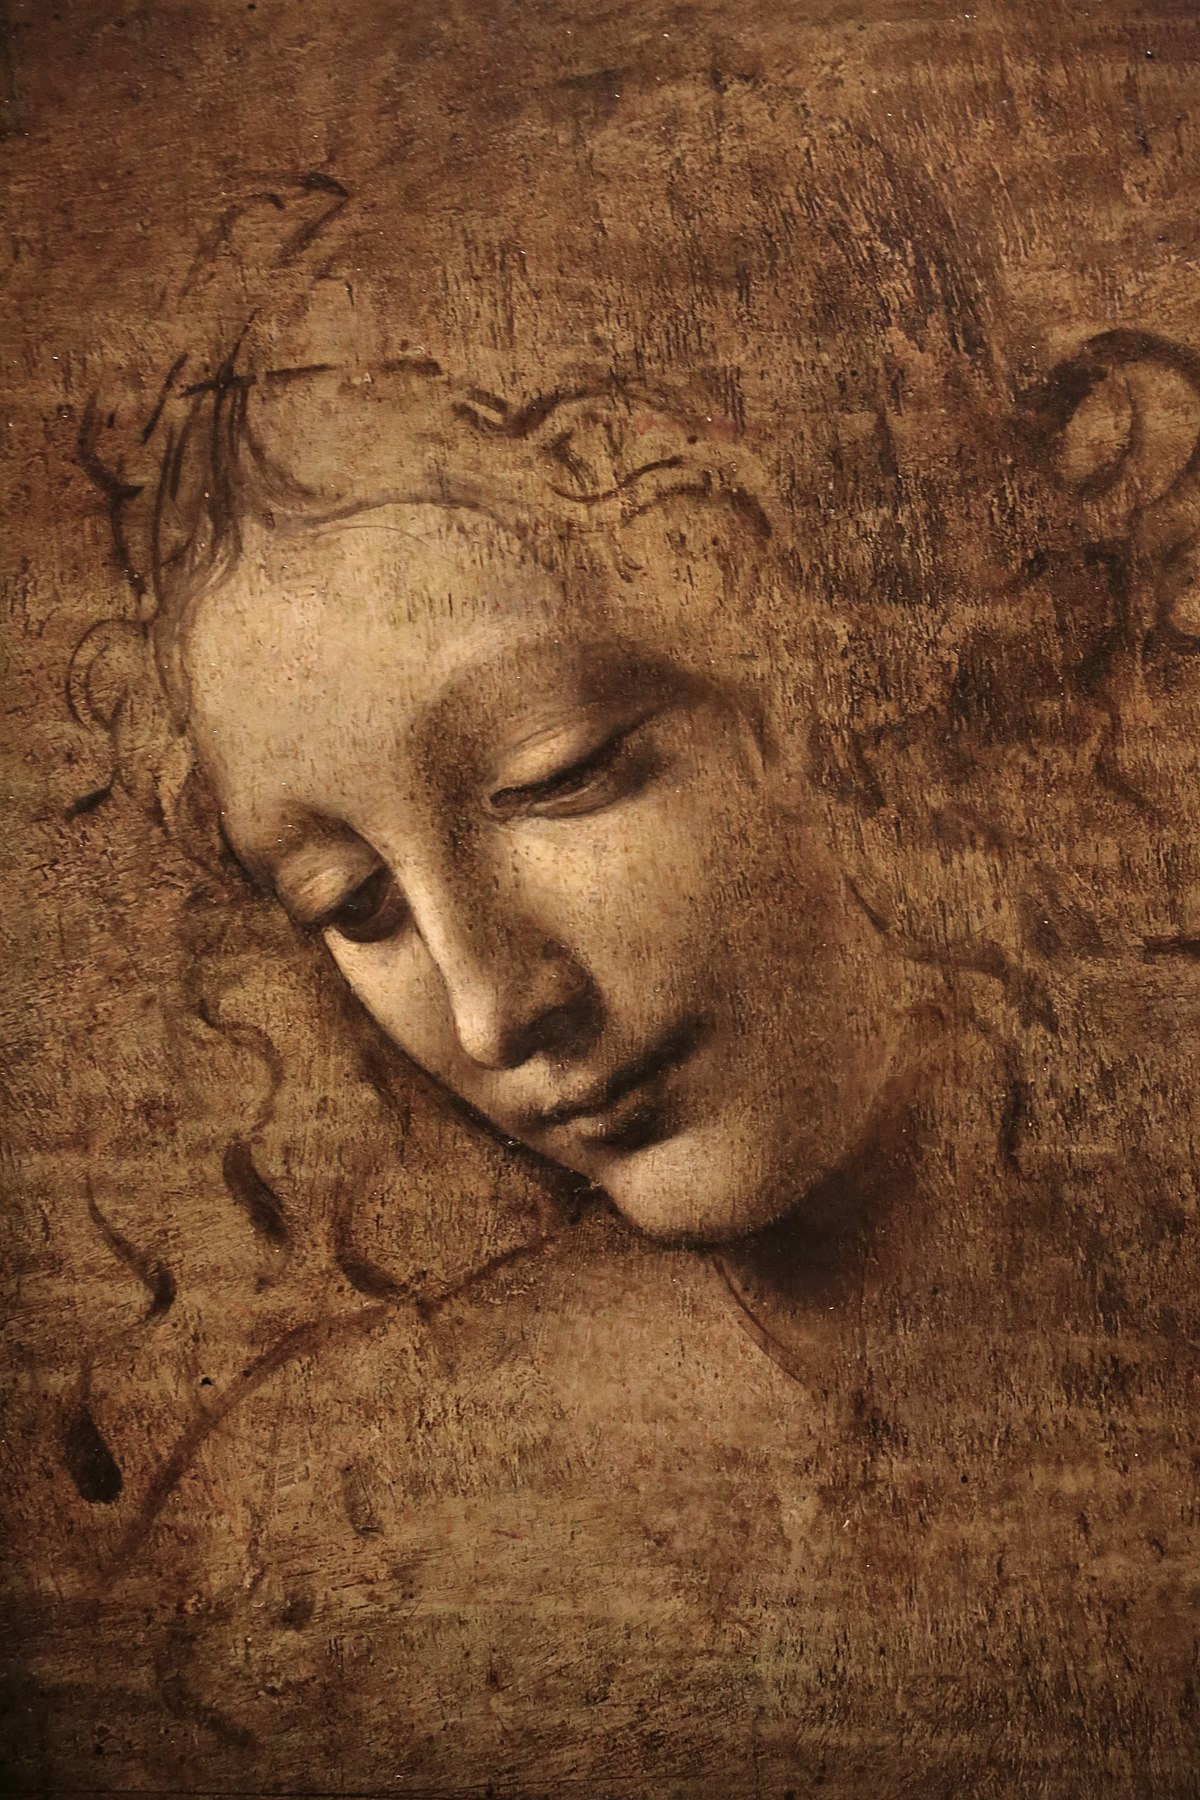
\includegraphics[width=0.6\textwidth]{Figuras/scapigliata}
		\captionsetup{margin=4cm}
		\caption[La Scapigliata]{La Scapiliata, una pintura al oleo sin ....}
		\label{fig:Scapigliata}
	\end{figure}
\end{lstlisting}


\begin{figure}[th]
	\centering
	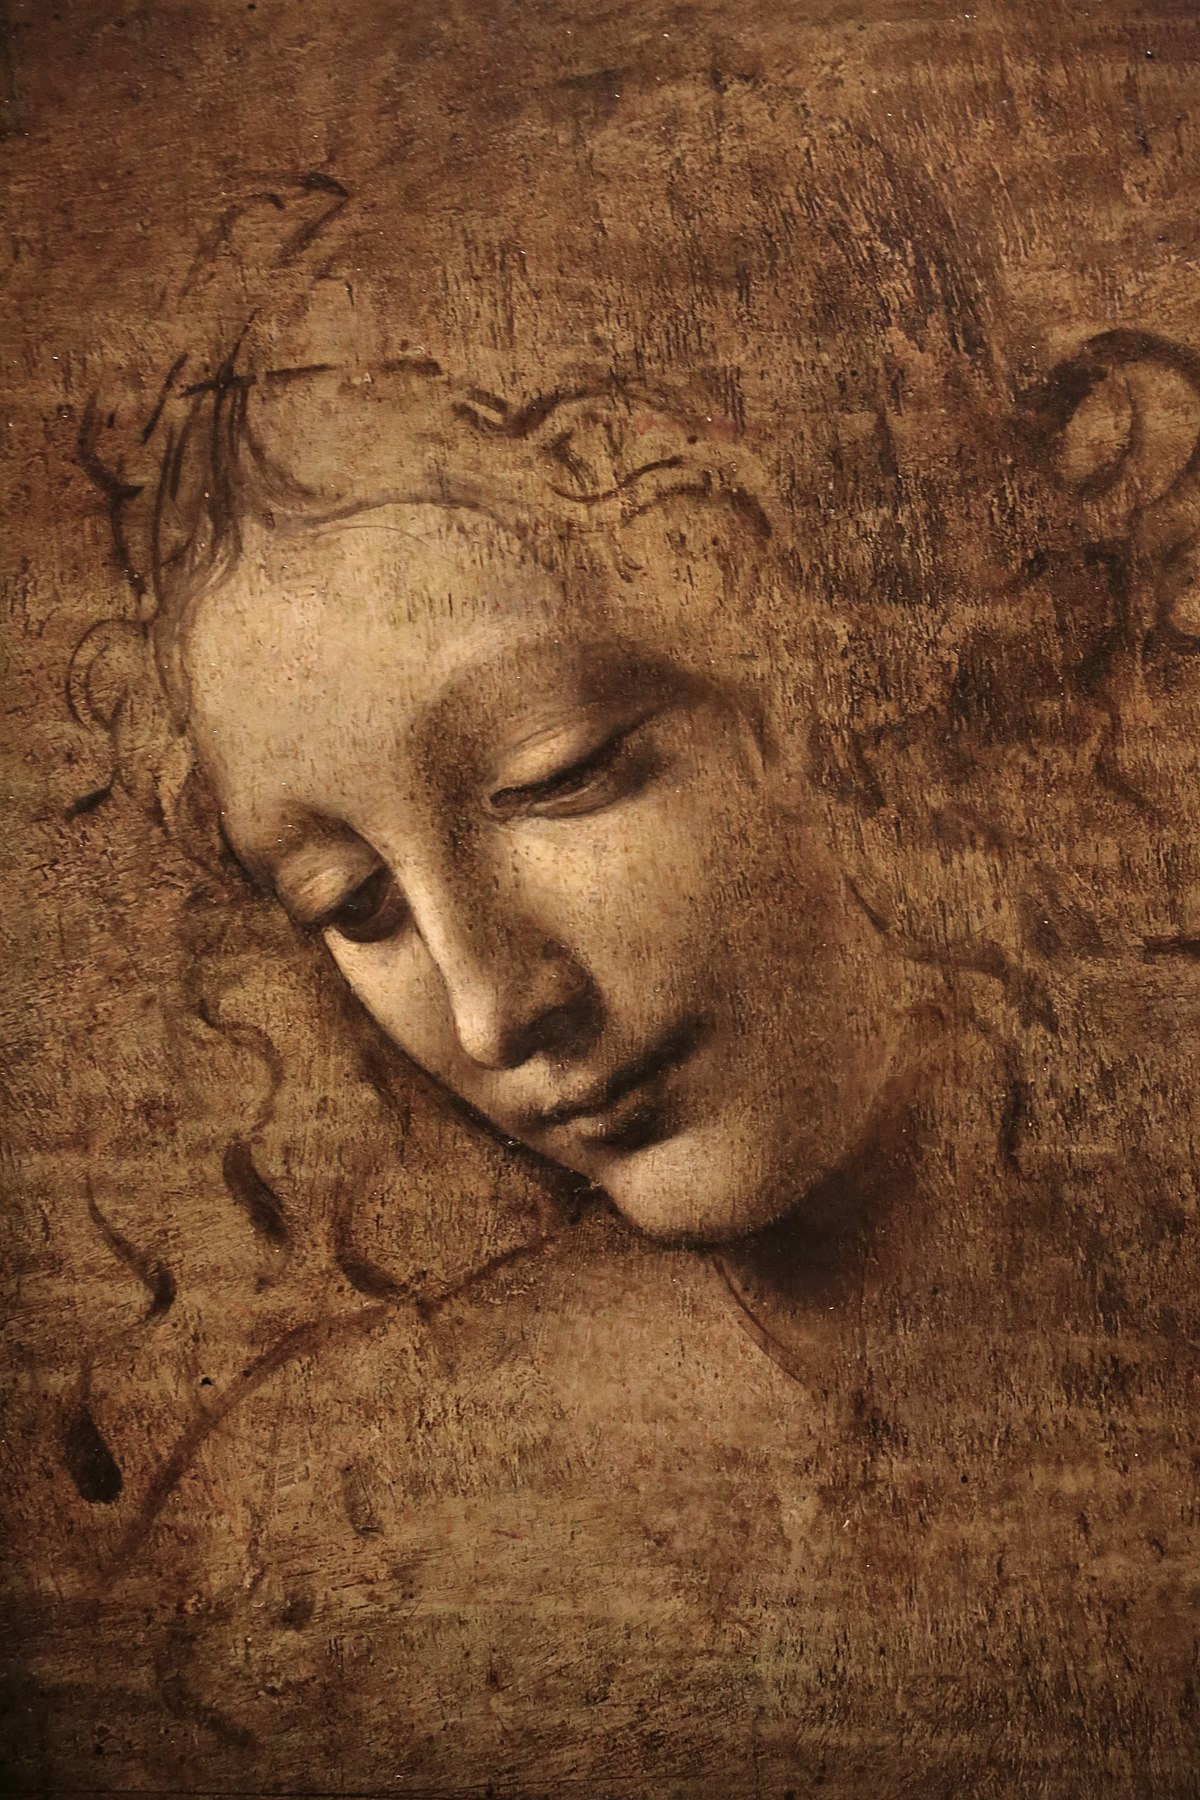
\includegraphics[width=0.4\textwidth]{Figuras/scapigliata}
	\captionsetup{margin=4cm}
	\caption[La Scapigliata]{La Scapiliata, una pintura al oleo sin terminar de fines del Renacimiento. No se conoce el autor, algunos historiadores atribuyen la autoría a Leonardo da Vinci.}
	\label{fig:Scapigliata}
\end{figure}

\LaTeX{} ubica las imágenes dependiendo del espacio que exista en la página. Algunas veces no hay lugar  suficiente para colocar una imagen en donde se declara \verb*|\begin{figure}|, en consecuencia \LaTeX{} la ubica en la parte superior de la siguiente página.
	
	Las figuras deben tener subtítulos los cuales deben ser explicativos y sintéticos.  También se pueden referenciar en el texto (como con la Figura ~ \ref{fig:Scapigliata}). La declaración \verb|\caption| posee dos partes, la primera parte, dentro de los corchetes es el título que aparecerá en el \emph{Índice de figuras}, por lo que debe ser breve. La segunda parte entre llaves debe contener el título más largo y la descripción de la figura. También se puede encuadrar el título de la figura referido al margen de la hoja, para ello debe emplear  \verb*|\captionsetup{margin=4cm}|. 
	
	
	
	También es posible cambiar la posición del comentario, por ejemplo, con la siguiente plantilla de código 
	
	\begin{lstlisting}[basicstyle=\small,tabsize=4]
		\begin{SCfigure}[0.5][h]
			\centering
			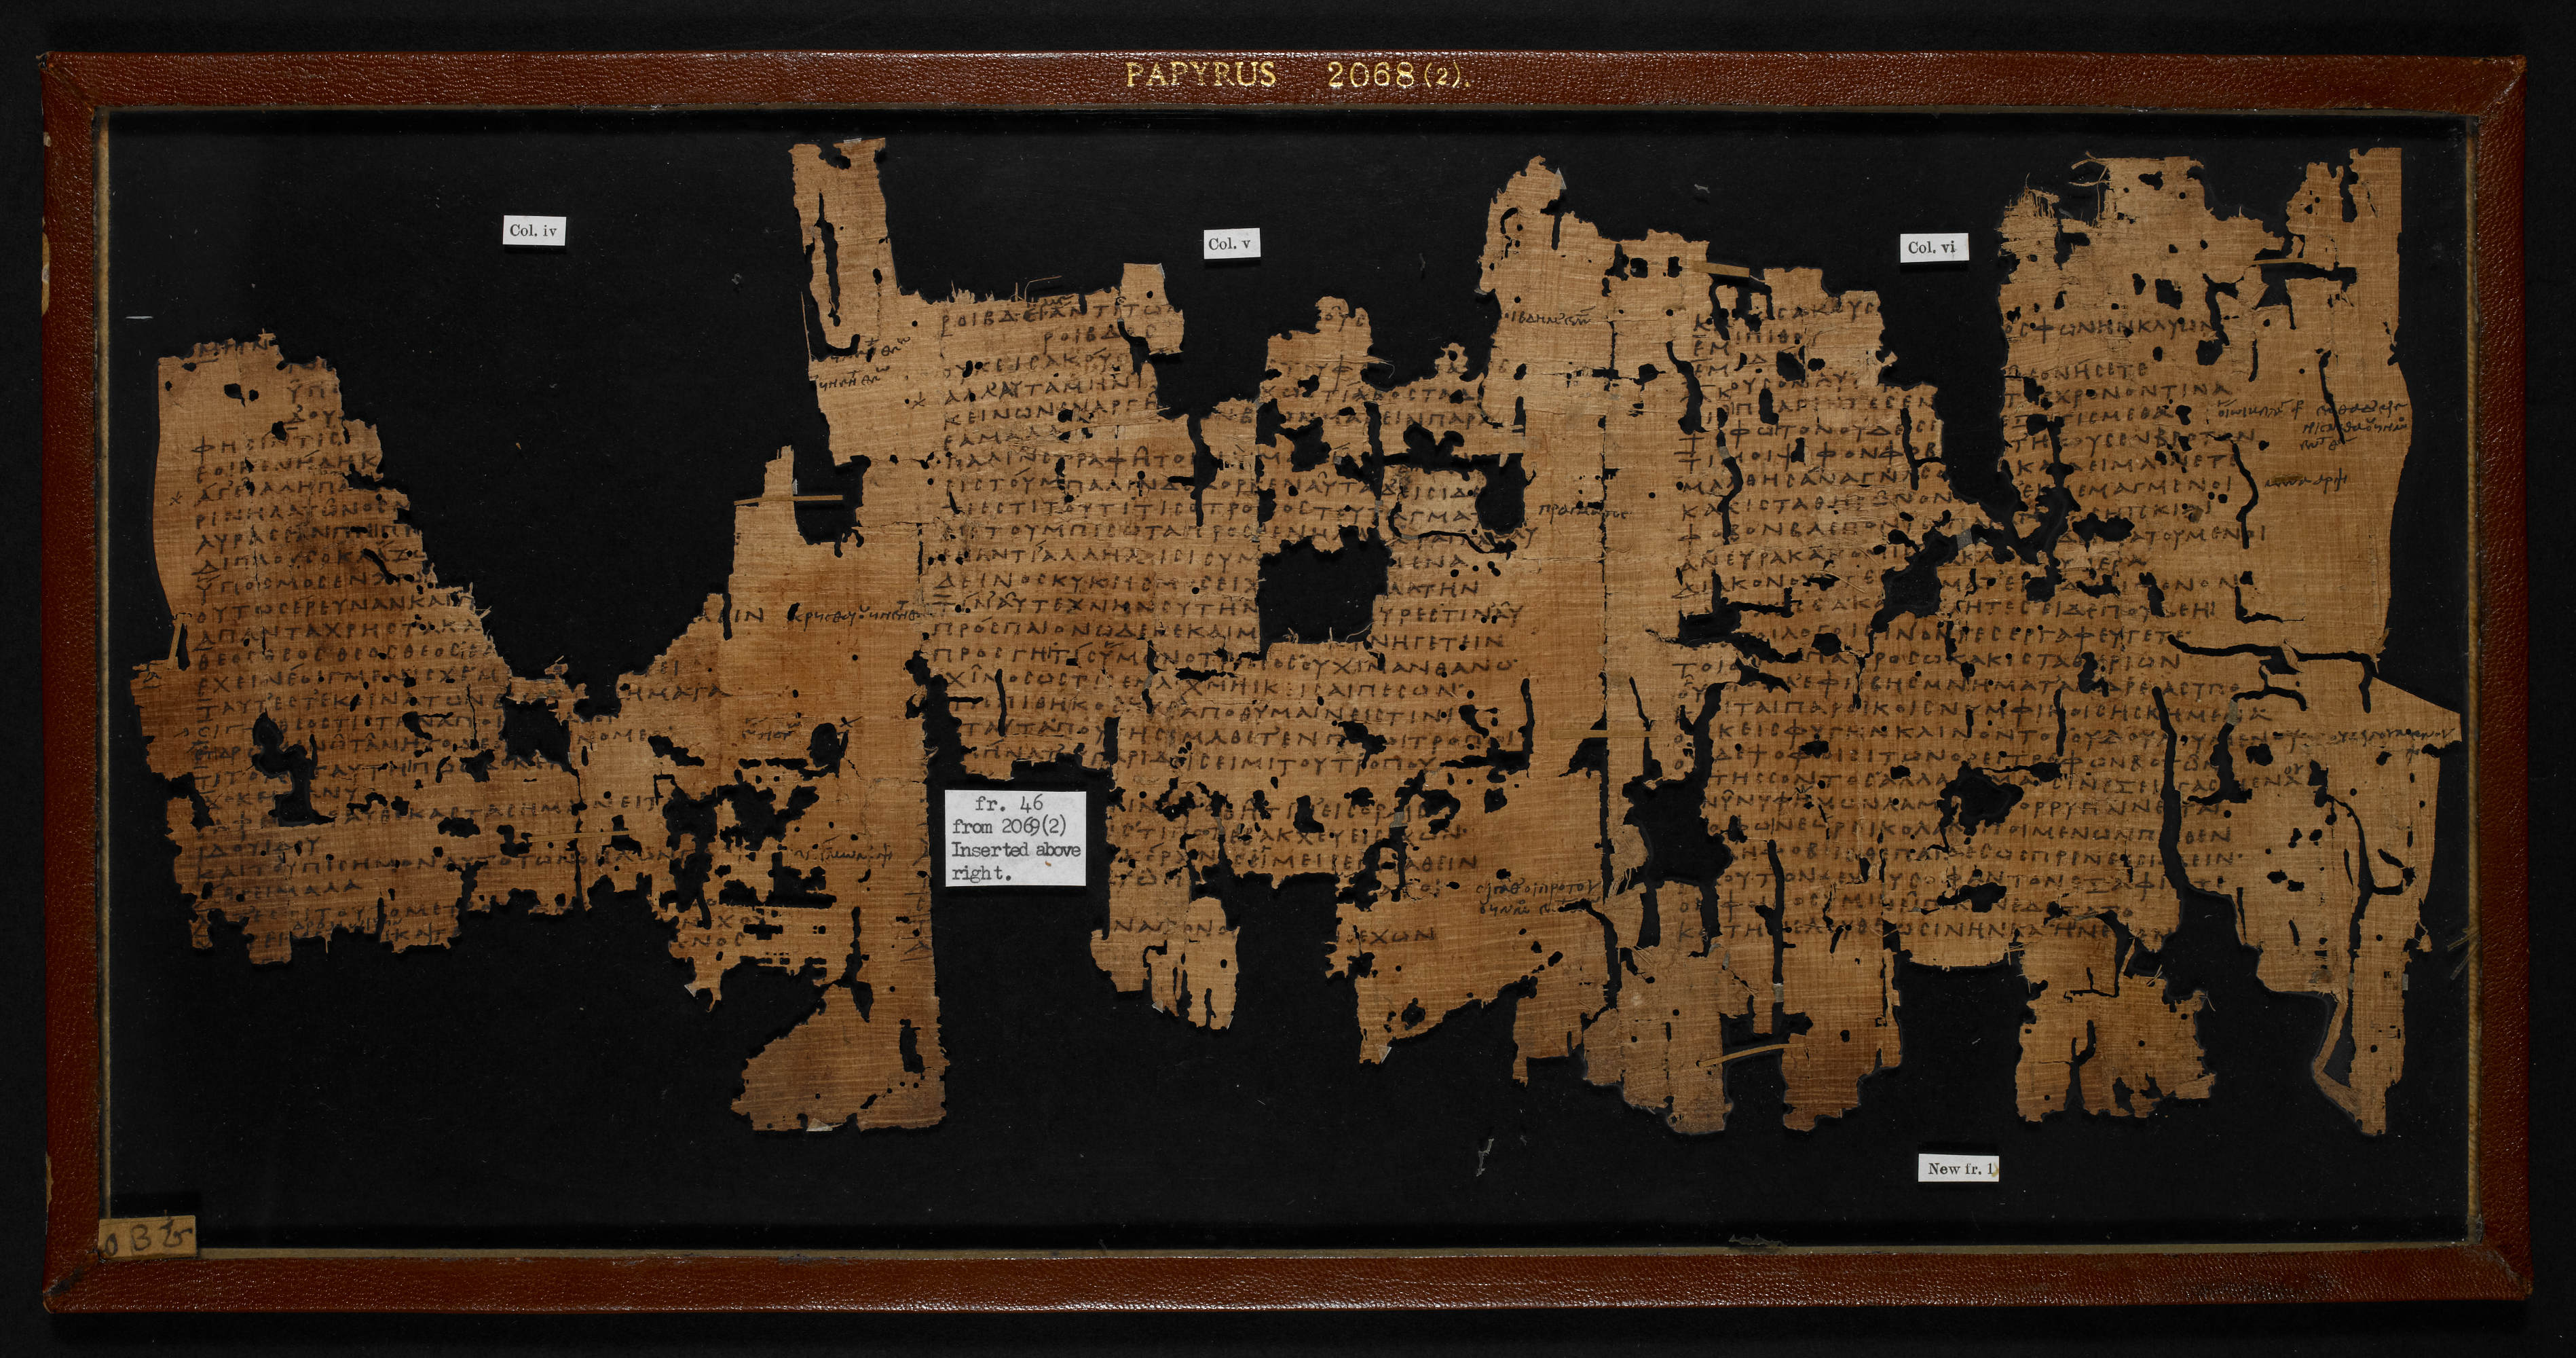
\includegraphics[width=0.6\textwidth]{Figuras/papyrus_sofocles}
			\caption[Ichneutae ....
			\label{fig:diag}
		\end{SCfigure}
	\end{lstlisting}
	
	se obtiene el resultado en la Figura \ref{fig:diag}, donde los comentarios de aparecen a la derecha.
	
	
	\begin{SCfigure}[0.5][h]
		\centering
		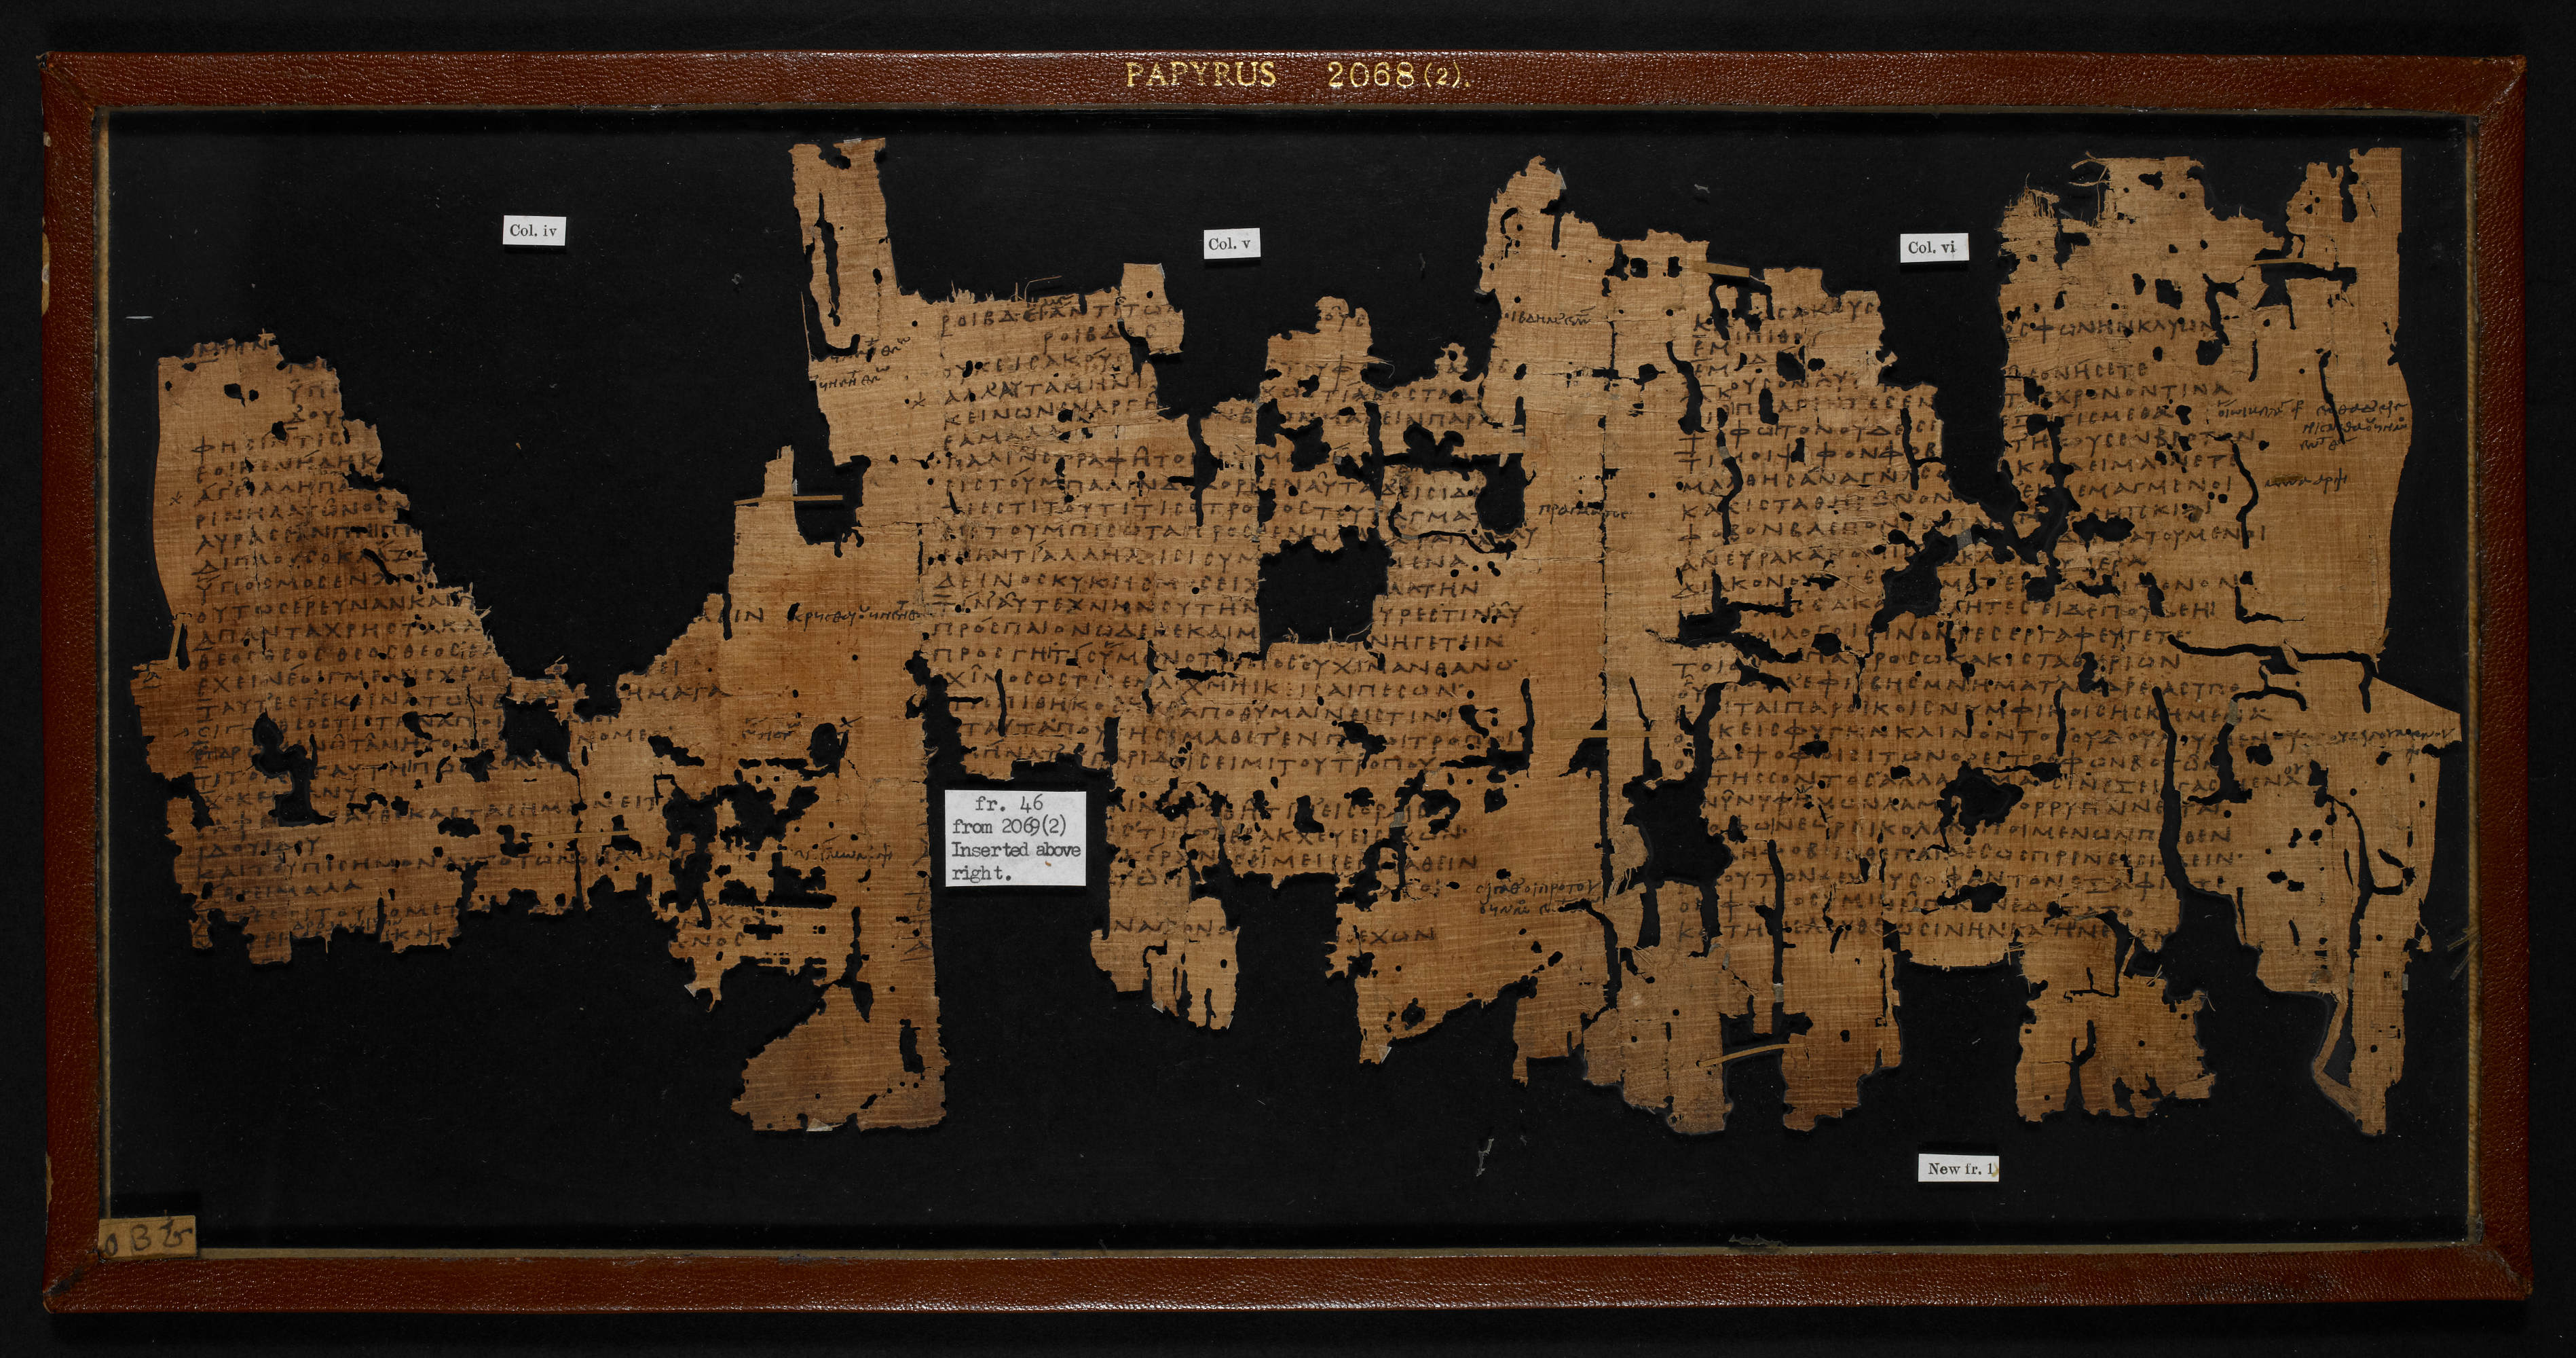
\includegraphics[width=0.6\textwidth]{Figuras/papyrus_sofocles}
		\caption[Ichneutae, o Perseguidores sátiros.]{Ichneutae, o Perseguidores sátiros. Fragmento del manuscrito del dramaturgo ateniense Sófocles. (Museo Británico)}
		\label{fig:diag}
	\end{SCfigure}
	
	%----------------------------------------------------------------------------------------
	\subsection{Una guía corta sobre Algoritmos}
	
	
	\begin{algorithm}[H]
		\label{alg:ejemplo1}
		\SetAlgoLined
		\KwData{$G=(X,U)$ de forma tal que $G^{tc}$ es un orden.}
		\KwResult{Escriba aquí el resultado }
		inicialización\;
		\While{condición}{
			instrucciones\;
			\eIf{condición}{
				instrucción1\;
				instrucción2\;
			}{
				instrucción3\;
			}
		}
		\caption{Cómo escribir una algoritmo}
	\end{algorithm}
	\
	
	Para la escritura de algoritmos existen diferentes posibilidades. En esta plantilla se empleó \verb*|\usepackage{listings}| para mostrar código desde un archivo. \emph{listings} permite listar código en diferentes lenguajes, por ejemplo, en el directorio \file{Codigo} se encuentra el archivo \file{c.c}.
	
	Mediante \verb*|\lstinputlisting[numbers=left, language=c]{Codigo/c.c}| se obtiene
	
	\lstinputlisting[numbers=left, language=c]{Codigo/c.c}
	
	\textbf{Un inconveniente con \emph{listings} es no tener una buena compatibilidad con UNICODE.}
	\\
	
	En muchos casos es preferible presentar un pseudocódigo que muestre en forma genérica la implementación de determinada deducción. Para ello el paquete \emph{algorithm2e} ofrece una alternativa muy conveniente. Se invita a mirar el archivo \file{Capitulos/cap3.tex} para observar el código que permite el resultado del Algoritmo \ref{alg:ejemplo1}
	
	
	
	%----------------------------------------------------------------------------------------

\section{Empiece a trabajar con esta Plantilla}

Si está familiarizado con \LaTeX{}, entonces debería explorar la estructura de directorios de la plantilla y luego proceder a cargar  su propia información en el archivo \file{tesina.tex}.  La sección \ref{CargaArchivo} en la página \pageref{CargaArchivo} le ayudará a hacer esto. Asegúrese de leer también la sección \ref{Convenciones} sobre las convenciones de tesis para aprovechar al máximo esta plantilla.

\subsection{Sobre esta Plantilla.}

Esta plantilla de tesis en \LaTeX{} tiene sus orígenes alrededor de un archivo de estilo \LaTeX{} creado por Steve R.  Gunn de la Universidad de Southampton (Reino Unido), Departamento de Electrónica y Ciencias de la Computación. Puede encontrar el archivo de estilo original en el sitio:
\url{http://www.ecs.soton.ac.uk/~srg/softwaretools/document/templates/}

A su vez, Sunil Patel tomó el archivo de clase \file{ecsthesis.cls} de Steve y lo modificó creando un marco esqueleto y una estructura de carpetas para colocar los archivos de tesis. La plantilla resultante se puede encontrar en el sitio de Sunil aquí: \url{http://www.sunilpatel.co.uk/thesis-template}

Se tomó la plantilla de Sunil, se la simplificó, y se adaptó a la presente plantilla, que conforma el modelo para la Tesina de Licenciatura de Sistemas de la Universidad Nacional de General Sarmiento. 
%----------------------------------------------------------------------------------------

\section{¿Qué incluye esta Plantilla?}

\subsection{Carpetas}
Esta plantilla viene como un único archivo zip que se expande a varios archivos y carpetas. Los nombres de las carpetas son en su mayoría autoexplicativos:

\keyword{Apendices}: esta es la carpeta donde coloca los apéndices. Cada apéndice debe ir en su propio archivo \file{.tex} separado. En el directorio se incluyen un ejemplo y una plantilla.

\keyword{Capítulos}: esta es la carpeta donde se encuentran el resumen y los capítulos de tesis. Una tesis suele tener unos seis capítulos, aunque no existe una regla estricta al respecto. Cada capítulo debe ir en su propio archivo \file{.tex} separado y se pueden dividir como:

\begin{itemize}
	\item \textit{Capítulo 1: Introducción}
	\item \textit{Capítulo 2: Revisión Bibliográfica}
	\item \textit{Capítulo 3: Materiales y Métodos}
	\item \textit{Capítulo 4: Resultados}
	\item \textit{Capítulo 5: Discusión}
	\item \textit{Capítulo 6:Conclusiones y  Recomendaciones}
\end{itemize}


Desde ya esta distribución puede no ser la más conveniente para los trabajos de tesis propuestos, y en ese caso, es conveniente modificarla. 

\keyword{Figuras} -- esta carpeta contiene todas las figuras de interés. En e las imágenes finales que se incluirán en el documento de tesis.

\keyword{Referencias} -- esta carpeta contiene el archivo de referencias bibliográficas \file{.bib}

\keyword{Codigo} -- en esta carpeta debe incluir aquellos archivos de código de programación que le interese mostrar.

\subsection{Archivos}

También se incluyen varios archivos, la mayoría de ellos son texto sin formato y puede ver su contenido en un editor de texto. Después de la compilación inicial, verá que \LaTeX{}  o BibTeX crearán más archivos auxiliares y que no se necesitan eliminar ni preocuparse por ellos.

\keyword{tesina.bib} -- este es un archivo importante que contiene toda la información bibliográfica y referencias que citará en la tesis para su uso con BibTeX. Puede escribirlo manualmente, pero hay programas de administración de referencias disponibles, los cuales permiten crearlo y administrarlo. Las bibliografías en \LaTeX{} son un tema extenso y es posible que deba leer sobre BibTeX antes de comenzar. Muchos sitios de publicaciones científicas y técnicas permiten exportar sus referencias en formato BibTeX, lo que facilita enormemente la compilación que se debe hacer.

\keyword{tesina.pdf} -- esta es su tesis bellamente compuesta (en formato de archivo PDF) creada por \LaTeX {}. Se proporciona  el PDF con la plantilla y, después de compilar la plantilla, debería obtener una versión idéntica.

\keyword{tesina.tex} -- este es un archivo importante. Este es el archivo que le dice a \LaTeX{} que debe compilar para producir su tesis como un archivo PDF. Contiene el marco y las construcciones que le dicen a \LaTeX{} cómo diseñar la tesis. Está muy comentado para que pueda leer lo que hace cada línea de código y por qué está allí. Después de poner su propia información en el bloque \emph{INFORMACIÓN DE TESIS}, ¡ha comenzado su tesis!
\\

Los archivos \emph{no} incluidos, pero creados por \LaTeX{} como archivos auxiliares incluyen:

\keyword{tesina.aux} -- este es un archivo auxiliar generado por \LaTeX{}, si se elimina \LaTeX{} simplemente lo regenera cuando ejecuta el archivo principal \file{.tex}.

\keyword{tesina.bbl} -- este es un archivo auxiliar generado por BibTeX, si se elimina, BibTeX simplemente lo regenera cuando ejecuta el archivo \file{tesina.aux}. Mientras que el archivo \file{.bib} contiene todas las referencias que usted incluyó, el archivo \file{.bbl} contiene las referencias que realmente se han citado en la tesis y se usa para construir la sección de bibliografía de la tesis. \emph{Es posible que cambios en el archivo \file{.bib} no se vean reflejados. Esto se puede deber a que no se recompila el archivo \file{.bbl}, en ese caso, se aconseja borrar al archivo \file{.bbl} para forzar una nueva compilación.}

\keyword{tesina.blg} -- este es un archivo auxiliar generado por BibTeX, si se elimina, BibTeX simplemente lo regenera cuando ejecuta el archivo principal \file{.aux}.

\keyword{tesina.lof} -- este es un archivo auxiliar generado por \LaTeX{}, si se elimina, \LaTeX{} simplemente lo regenera cuando ejecuta el archivo principal \file{.tex}. Le dice a \LaTeX{} cómo construir la sección \emph{Lista de figuras}.

\keyword{tesina.log} -- este es un archivo auxiliar generado por \LaTeX{}, si se elimina \LaTeX{} simplemente lo regenera cuando ejecuta el archivo principal \file{.tex}. Contiene mensajes de \LaTeX{}, si recibe errores y advertencias de \LaTeX {}, estarán en este archivo \file{.log}.

\keyword{tesina.lot} -- este es un archivo auxiliar generado por \LaTeX{}, si se elimina \LaTeX{} simplemente lo regenera cuando ejecuta el archivo principal  file{.tex}. Le dice a \LaTeX{} cómo construir la sección \emph{Lista de tablas}.

\keyword{tesina.out} -- este es un archivo auxiliar generado por \LaTeX{}, si se elimina \LaTeX{} simplemente lo regenera cuando ejecuta el archivo principal  \file{.tex}.

Entonces, de esta larga lista, solo los archivos con las extensiones \file{.bib}  y \file{.tex} son los más importantes. Los otros archivos auxiliares se pueden ignorar o eliminar ya que \LaTeX{} y BibTeX los regenerarán.

%----------------------------------------------------------------------------------------

\section{Cargando la Plantilla con sus datos en  el archivo \file{tesina.tex} }\label{CargaArchivo}


Deberá personalizar la plantilla de tesis y hacerla suya completándola con  su propia información. Esto se hace editando el archivo \file{tesina.tex} en un editor de texto o en su entorno \LaTeX{} favorito.

Abra el archivo y desplácese hacia abajo hasta el tercer bloque grande titulado \emph{DATOS DE PORTADA} donde puede ver las entradas para \emph{Nombre de la Universidad}, \emph{Nombre del Instituto}, etc \ldots

Complete la información sobre usted, grupo e institución. También puede insertar enlaces web, si lo hace, asegúrese de utilizar la URL completa, incluido el código \emph{http://}. Si no desea que estos estén vinculados, simplemente elimine \verb|\href{url}{nombre}| y solo deje el nombre.

\

A continuación se declara la lista de \emph{Acrónimos y Glosario}. Por el repetido uso en el texto de ciertas palabras, o por existir un manera tradicional de escribir una significación, se emplean acrónimos para facilitar la escritura. Son palabras formadas por sílabas o abreviaturas que representan otras palabras y por lo tanto tienen significado. Un ejemplo es \emph{UNGS}, el acrónimo de \emph{Universidad Nacional de General Sarmiento}, otro ejemplo muy común es  \acs{id} (\verb*|\acs{id}|), el cuál significa  \acl{id} (\verb*|\acl{id}|), y se encuentra indicado en la \emph{Lista de Abreviaciones}.  

Por su parte, el \emph{Glosario} es un catálogo alfabetizado de símbolos, palabras y expresiones que son particulares del texto, difíciles de comprender, donde se las lista junto con su significado o algún comentario, por ejemplo \acs{angelsperarea} (\verb*|\acs{angelsperarea}|), la \emph{densidad superficial de ángeles}, se encuentra definido en el glosario.

En el encabezado de \file{tesina.tex} en el bloque \emph{DECLARACIÓN DE ACRÓNIMOS Y GLOSARIO} se declaran los acrónimos y definiciones que se van a emplear, o no, en el cuerpo de la tesis. Aquellos que se emplearan quedan habilitados para conformar la \emph{Lista de Abreviaciones} y el \emph{Glosario}. 

Estos índices son importantes ya que facilitan al lector la identificación y significado de las abreviaciones que se leen durante el texto. 

\

Cuando haya hecho todas las modificaciones, guarde el archivo y recompile. Toda la información que completó ahora debería estar en el PDF, con los enlaces web. 



%----------------------------------------------------------------------------------------

\section{El archivo \code{tesina.tex} Explicado.}

El archivo \file{main.tex} contiene la estructura de la tesis. Hay muchos comentarios escritos que explican qué páginas, secciones y formato está creando el código \LaTeX{}. Cada elemento principal del documento se divide en bloques comentados con títulos en mayúsculas para que sea obvio lo que está haciendo el  fragmento de código que le sigue. Inicialmente parece haber mucho código \LaTeX{}, pero es declaración de  formato, que ha sido arreglado para que Ud. no tenga que hacerlo.

Luego viene una página que contiene una cita, puede reemplazarla por una cita de su científico, autor, persona, etc. favoritos. Asegúrese de poner el nombre de la persona de quien se tomó la cita.

A continuación, se encuentra la página de \emph{Resumen} que sintetiza su trabajo de manera condensada y casi se puede utilizar como un documento independiente para describir lo que se ha hecho. El Resumen se escribe en el archivo \file{resumen.tex} que se encuentra en la carpeta \emph{Capitulos}


Luego vienen los agradecimientos. En esta página, escriba sobre todas las personas a las que desea agradecer (sin olvidar a los padres, compañeros y a su director y/o supervisor).

Las páginas de contenido, la lista de figuras y las tablas \LaTeX{}  las arma por Ud. en base a la información de estructura que se provee al escribir la tesis, y no es necesario crearlas o editarlas manualmente. En cuanto a la lista de símbolos, abreviaturas y definiciones, debe procurarse que queden ordenadas alfabéticamente, separando alfabetos romanos y griego (esto \emph{no} se hace automáticamente). 

La siguiente página contiene una dedicatoria de una línea. ¿A quién dedicará su tesis?

Finalmente, está el bloque donde se incluyen los capítulos. Elimine el  carácter  \code{\%} para des-comentar las líneas mientras escribe los capítulos. Cada capítulo debe escribirse en su propio archivo, colocarse en la carpeta \emph{Capitulos} y denominarse \file{cap1.tex}, \file{cap2.tex}, etc \ldots De manera similar, para los apéndices, elimine los comentarios de las líneas según los necesite. Cada apéndice debe ir en su propio archivo y colocarse en la carpeta \emph{Apendices}.

Después del preámbulo, capítulos y apéndices finalmente viene la bibliografía. El estilo de bibliografía (llamado \option{plain}) se utiliza para la bibliografía y es un estilo con todas las funciones, e  incluso incluye la posibilidad de  enlaces DOI (así sea agregada en las notas). Su lector estará agradecido al descubrir que una referencia a un artículo está a solo un clic de distancia. Por supuesto, esto depende de que usted ponga la información de la URL en el archivo BibTeX en primer lugar.


%----------------------------------------------------------------------------------------



\section{Conclusión del Capítulo \ref{Cap_Plantilla} }

Ha llegado al final de esta mini-guía. Ahora puede cambiar el nombre o sobrescribir este archivo PDF y comenzar a escribir su propio \file{Capitulo/cap1.tex} y el resto de su tesis.


 % Guía de uso de la plantilla (referencia)

\afterpage{\blankpage}

%-----------------------------------------------------------------------------------
% Anexos 
%-----------------------------------------------------------------------------------
\begin{appendices}
\startchapter[title={Diagramas}, reference=Anexo_Diagramas]

% TODO: completar

\stopchapter
 % Diagramas
\startchapter[title={Pseudocódigos}, reference=Anexo_Pseudocodigos]

%----------------------------------------------------------------------------------------
\startsection[title={Modelo Lineal Monolítico}, reference=sec:pseudo_monolitico]

% TODO: completar

\stopsection

%----------------------------------------------------------------------------------------
\startsection[title={Modelo Lineal En Dos Etapas (Split)}, reference=sec:pseudo_split]

% TODO: completar

\stopsection

%----------------------------------------------------------------------------------------
\startsection[title={Hill Climbing}, reference=sec:pseudo_hc]

% TODO: completar

\stopsection

%----------------------------------------------------------------------------------------
\startsection[title={Ant Colony Optimization}, reference=sec:pseudo_aco]

% TODO: completar

\stopsection
\stopchapter
 % Pseudocódigos
\end{appendices}


%-----------------------------------------------------------------------------------
% Referencias
%-----------------------------------------------------------------------------------
\bibliographystyle{plain}
\bibliography{Referencias/tesina.bib} %tesina.bib
\addcontentsline{toc}{chapter}{Bibliografía}

\end{document}
